%\VignetteIndexEntry{PPBstats}
%\VignetteEngine{knitr::knitr}

\documentclass{article}\usepackage[]{graphicx}\usepackage[]{color}
%% maxwidth is the original width if it is less than linewidth
%% otherwise use linewidth (to make sure the graphics do not exceed the margin)
\makeatletter
\def\maxwidth{ %
  \ifdim\Gin@nat@width>\linewidth
    \linewidth
  \else
    \Gin@nat@width
  \fi
}
\makeatother

\definecolor{fgcolor}{rgb}{0.345, 0.345, 0.345}
\newcommand{\hlnum}[1]{\textcolor[rgb]{0.686,0.059,0.569}{#1}}%
\newcommand{\hlstr}[1]{\textcolor[rgb]{0.192,0.494,0.8}{#1}}%
\newcommand{\hlcom}[1]{\textcolor[rgb]{0.678,0.584,0.686}{\textit{#1}}}%
\newcommand{\hlopt}[1]{\textcolor[rgb]{0,0,0}{#1}}%
\newcommand{\hlstd}[1]{\textcolor[rgb]{0.345,0.345,0.345}{#1}}%
\newcommand{\hlkwa}[1]{\textcolor[rgb]{0.161,0.373,0.58}{\textbf{#1}}}%
\newcommand{\hlkwb}[1]{\textcolor[rgb]{0.69,0.353,0.396}{#1}}%
\newcommand{\hlkwc}[1]{\textcolor[rgb]{0.333,0.667,0.333}{#1}}%
\newcommand{\hlkwd}[1]{\textcolor[rgb]{0.737,0.353,0.396}{\textbf{#1}}}%

\usepackage{framed}
\makeatletter
\newenvironment{kframe}{%
 \def\at@end@of@kframe{}%
 \ifinner\ifhmode%
  \def\at@end@of@kframe{\end{minipage}}%
  \begin{minipage}{\columnwidth}%
 \fi\fi%
 \def\FrameCommand##1{\hskip\@totalleftmargin \hskip-\fboxsep
 \colorbox{shadecolor}{##1}\hskip-\fboxsep
     % There is no \\@totalrightmargin, so:
     \hskip-\linewidth \hskip-\@totalleftmargin \hskip\columnwidth}%
 \MakeFramed {\advance\hsize-\width
   \@totalleftmargin\z@ \linewidth\hsize
   \@setminipage}}%
 {\par\unskip\endMakeFramed%
 \at@end@of@kframe}
\makeatother

\definecolor{shadecolor}{rgb}{.97, .97, .97}
\definecolor{messagecolor}{rgb}{0, 0, 0}
\definecolor{warningcolor}{rgb}{1, 0, 1}
\definecolor{errorcolor}{rgb}{1, 0, 0}
\newenvironment{knitrout}{}{} % an empty environment to be redefined in TeX

\usepackage{alltt}

% to draw on figure or create figures
\usepackage{tikz}
\usepackage{pstricks}

\usetikzlibrary{shapes,arrows}
\graphicspath{{./figures/}}
\usepackage{wrapfig}

\usepackage{multicol}

\usepackage[utf8]{inputenc}

\usepackage[T1]{fontenc}
\usepackage[top=2cm, bottom=2cm, left=3cm, right=2cm]{geometry}
\setcounter{secnumdepth}{3}
\setcounter{tocdepth}{3}
\usepackage{url}
\usepackage[round]{natbib}
\usepackage[a4paper=true, colorlinks=true, linkcolor=black,urlcolor=blue,citecolor=black]{hyperref}


\usepackage{colortbl, xcolor}
\usepackage{float}

\newcommand{\pack}{\texttt{PPBstats}}
\newcommand{\R}{\texttt{R}}
\newcommand{\versionnumber}{0.11}
\IfFileExists{upquote.sty}{\usepackage{upquote}}{}
\begin{document}



\pagestyle{empty}
\begin{center}
\Huge{\pack } \\
\Large{An \R~package to perform analysis found within PPB programmes regarding network of seeds circulation, agronomic trials, organoleptic tests and molecular experiments}

~\\

\warning{Be aware that this package is under development and test: do not 100\% trust the functions!!! You're welcome to contribute. See for more \href{https://github.com/priviere/PPBstats/releases/download/v0.22/contribute_PPBstats.pdf}{here} details.}


~\\

version \versionnumber \\

~\\
\today

~\\~\\

Pierre Rivi\`ere\textsuperscript{1,2} \hspace{.5cm} 
Gaelle Van Frank\textsuperscript{2} \hspace{.5cm}
Olivier David\textsuperscript{3}  \hspace{.5cm} 
Facundo Muñoz\textsuperscript{4}
\\
~\\~\\ 
\end{center}

\vfill

\noindent\textsuperscript{1} R\'eseau Semences Paysannes, 3 avenue de la gare, F-47190 Aiguillon, France \\
\textsuperscript{2} INRA, UMR 0320, Génétique Quantitative et Evolution, Ferme du Moulon F-91190 Gif sur Yvette, France \\
\textsuperscript{3} INRA, UR 1404 Unité Mathématiques et Informatique Appliquées du Génome à l'Environnement, F-78352 Jouy-en-Josas, France \\ 
\textsuperscript{4} INRA, Centre Val de Loire, Unité Amélioration, Génétique et Physiologie Forestières, F-45075 Orléans, France \\ 
\textbf{Contact:} \href{mailto:pierre@semencespaysannes.org}{pierre@semencespaysannes.org} \\

\vfill

\noindent\textbf{Contributions:} \\
PR coordinates the package development, wrote the \texttt{R} functions and the vignette \\
GVF test the package and updated the code regarding Sections~\ref{ammi}, \ref{gge}, \ref{model_1}, \ref{model_2} and \ref{variance_intra} \\
OD wrote the \texttt{JAGS} code and reviewed the \texttt{R} code and the vignette regarding Sections~\ref{model_1}, \ref{model_2} and \ref{variance_intra} \\
FM reformated and improved all the code especially regarding S3 methods and reviewed and improved the vignette \\

\vfill

\begin{center}
Copyright Réseau Semences Paysannes and Institut National de la Recherche Agronomique \\
\href{http://creativecommons.org/licenses/by-nc-sa/4.0/}{Licence creative commons BY-NC-SA 4.0} \\
\vspace{.25cm}
\href{http://creativecommons.org/licenses/by-nc-sa/4.0/}{
\includegraphics[width=.15\textwidth]{cc-by-nc-sa}}
\end{center}

\clearpage

\begin{wrapfigure}{l}{.15\textwidth}
\begin{center} \vspace{-20pt}

\includegraphics[width=.15\textwidth]{Logo-RSP}
\end{center} \vspace{-20pt}
\end{wrapfigure}
\noindent
Le Réseau Semences Paysannes (the French Farmers' Seeds Network (RSP)), created in 2003, brings together a great diversity of collectives and people who preserve farmers' seeds in fields, orchards, vineyards and gardens. They are involved in supporting the consolidation of local initiatives to maintain and renew cultivated biodiversity through Community Seeds Systems. Over 80 organizations have come together to promote and develop farmers' seeds, and to protect farmers' rights over their seeds. \\
\url{www.semencespaysannes.org} (in french).


\vfill

\begin{wrapfigure}{l}{.15\textwidth}
\begin{center} \vspace{-20pt}

\includegraphics[width=.15\textwidth]{Logo-UMRGV}
\end{center} \vspace{-20pt}
\end{wrapfigure}
\noindent
The Diversity, Evolution and Adaptation of Populations (DEAP) team led by Isabelle Goldringer is part of INRA UMR 0320 Quantitative Genetic and Evolution.
Its work is based on the analysis of the genetic and evolutionary mechanisms underlying evolution and adaptation of crop populations.
DEAP develops strategies for on farm management of crop genetic diversity and
for plant breeding (evolutionary and/or participatory) adated to organic and low input agriculture.
Assessing the benefits of in-field genetic diversity (variety mixtures, populations) and designing
/ breeding optimized mixtures adapted to local conditions are also key research objectives.\\
\url{http://moulon.inra.fr/index.php/en/team/deap}


\vfill


\begin{wrapfigure}{l}{.15\textwidth}
\begin{center} \vspace{-20pt}

\includegraphics[width=.15\textwidth]{Logo-maiage}
\end{center} \vspace{-20pt}
\end{wrapfigure}
\noindent
The INRA UR1404 MaIAGE research laboratory gathers mathematicians, computer scientists, bioinformaticians and biologists to tackle problems coming from biology, agronomy and ecology; The addressed questions may concern processes at very different levels: molecular, cellular or multicellular, individual, populations, ecosystems oy landscapes. 
MaIAGE develops original methods in mathematics, statistics and computer science which are generic or driven by specific biological problems. A particular attention is paid to develop and make available softwares, databases, ontologies and web services so that biologists can use them easily to analyze their data or to mine the scientific literature.\\
\url{http://maiage.jouy.inra.fr/?q=en/home}



\newpage

\tableofcontents

\vfill

\begin{center}
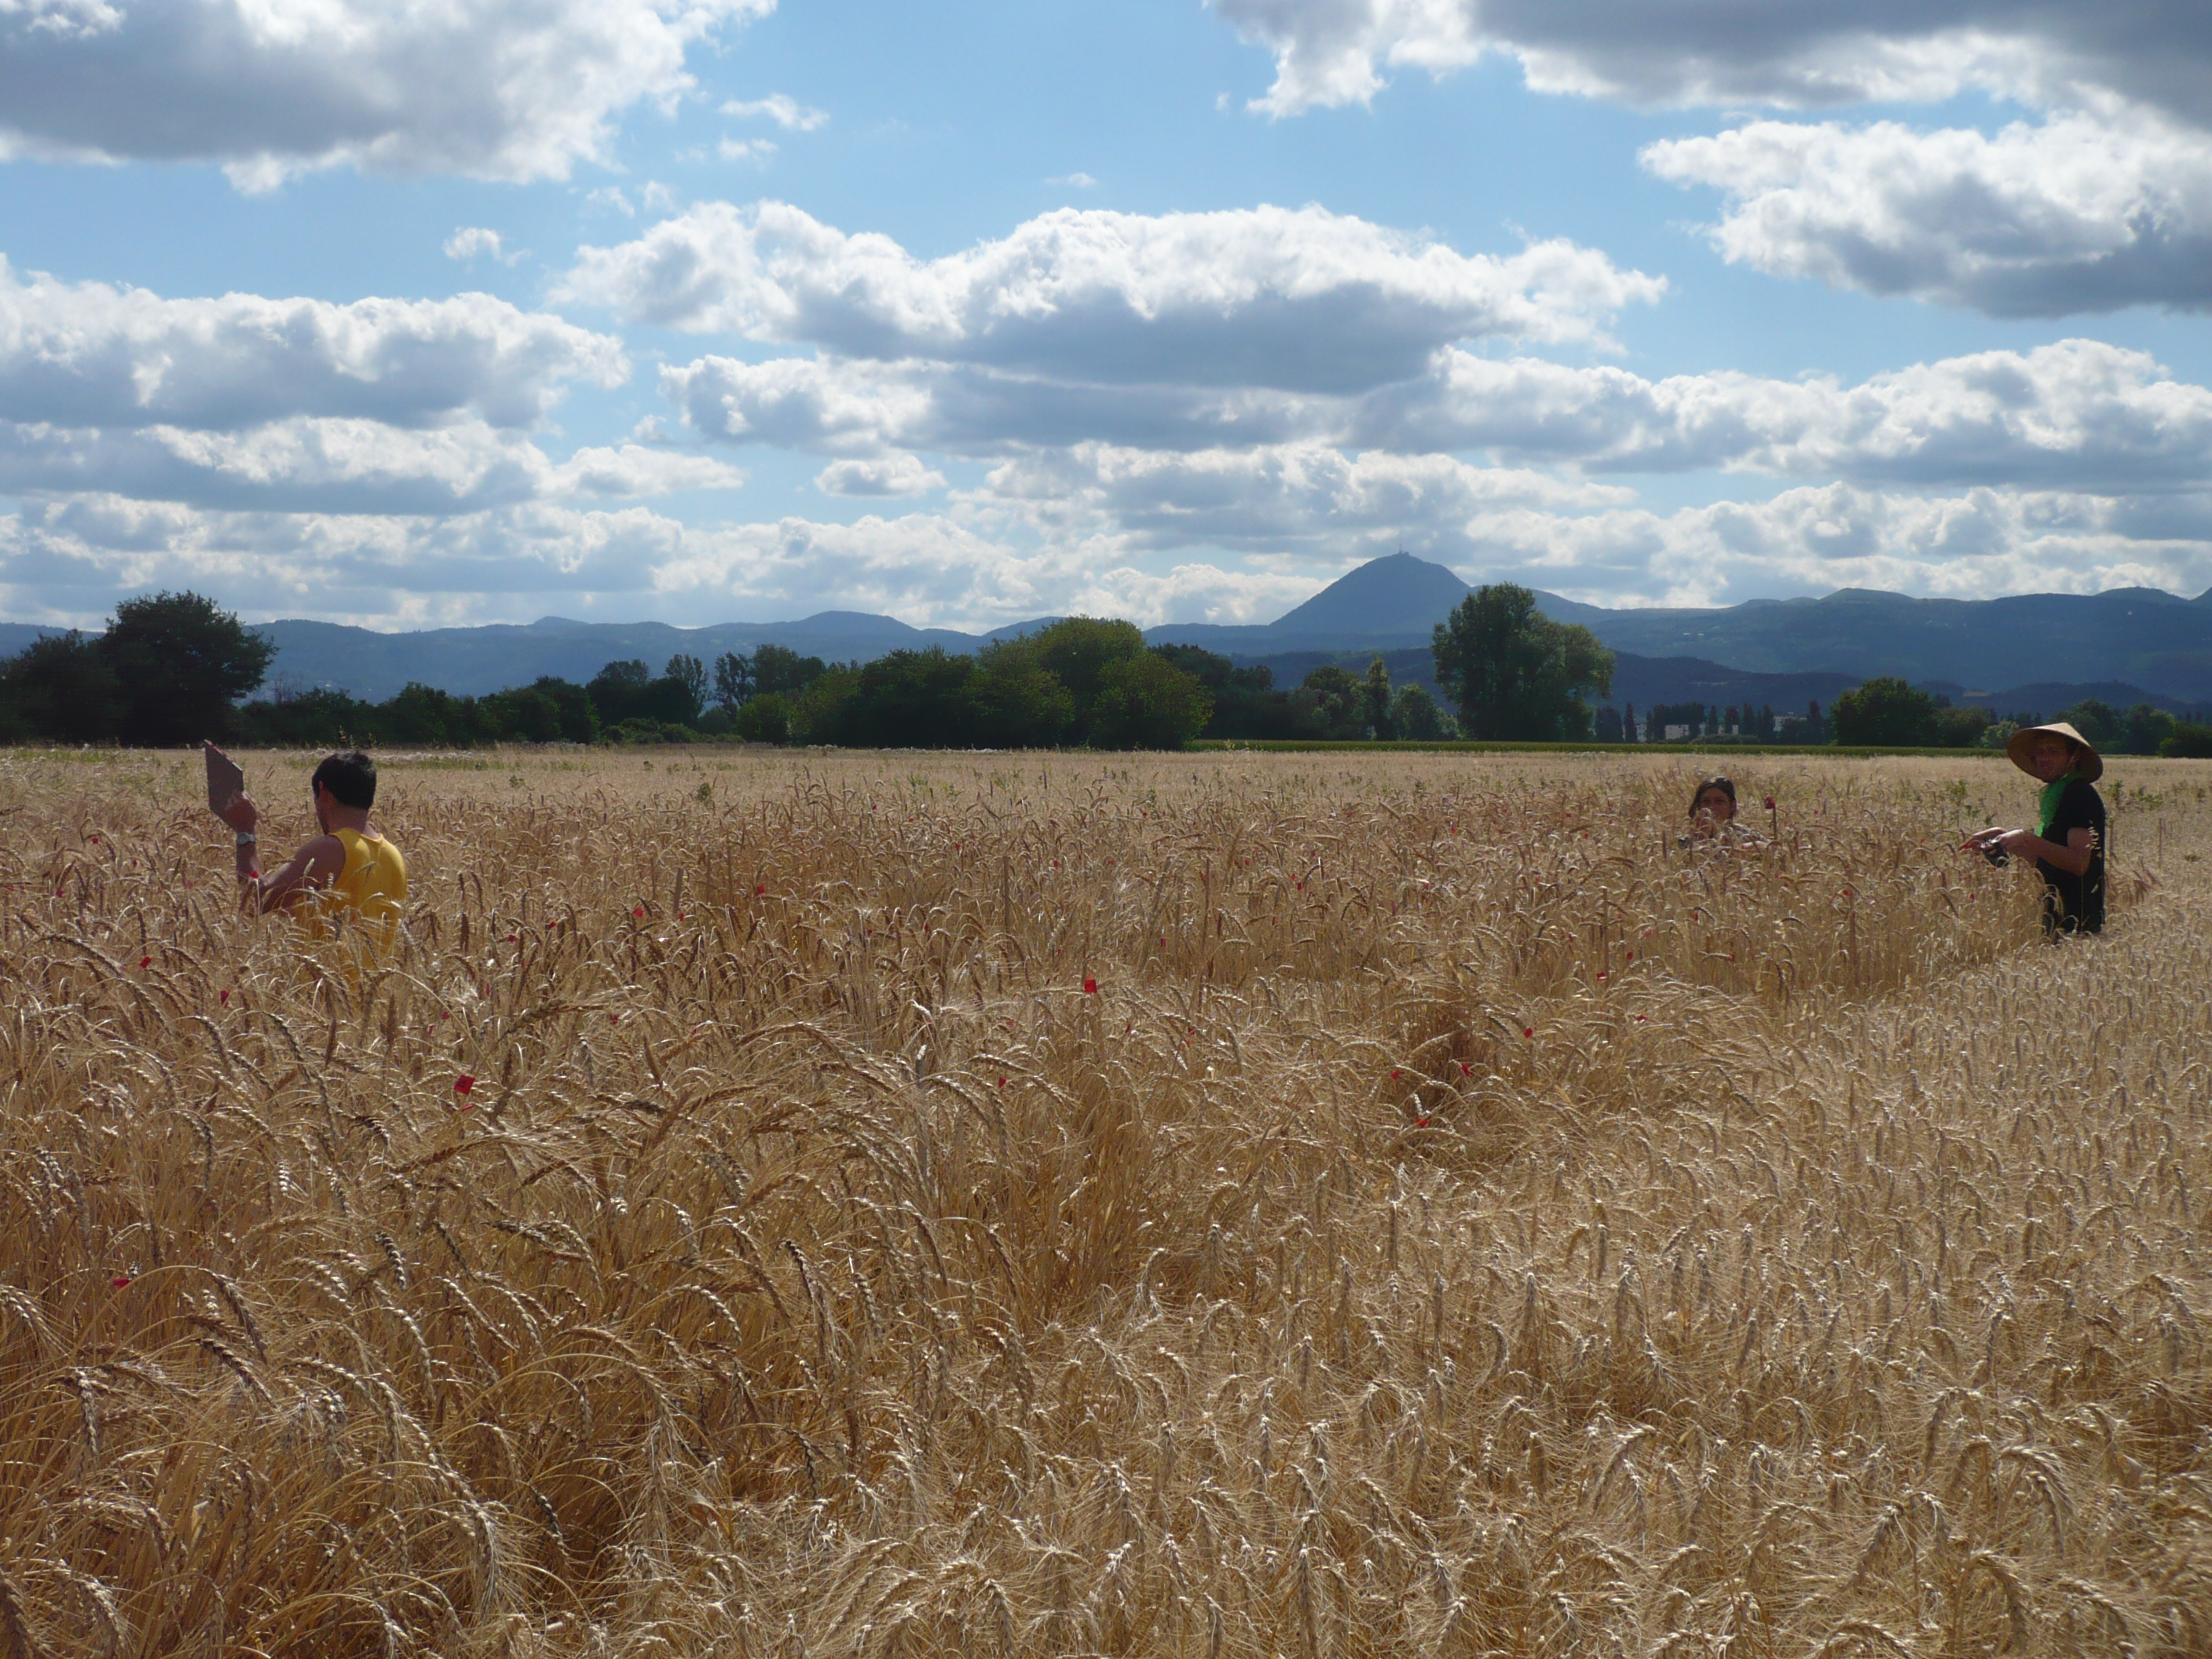
\includegraphics[width=.8\textwidth]{wheat} \\
Wheat trials on farm within our participatory plant breeding programme, summer 2012, Auvergne, France. \\
CC-BY-NC-SA. Pierre Rivière.
\end{center}

\newpage
\pagestyle{plain}


\section{Philosophy of \pack}

\pack~aims to facilitate the implementation of statistical methods described in \citet{riviere_hierarchical_2015} and \citet{riviere_hierarchical_2015-1}.
These methods aim to analyse highly unbalanced datasets that can be found in decentralized participatory plant breeding (PPB).

It has been developped for dataset with two types of farms, regional and satellite, based on their experimental design.

Regional farms had several populations (i.e. a germplasm in an environment) in two or more blocks with populations replicated in each block.
Satellite farms had no block and one germplasm replicated twice.
Farmers chose the other populations to be sown that were not replicated (Figure \ref{plan_SF_RF}).
The number of populations may vary between farms.

\begin{figure}[H]
        \begin{center}
                \begin{tabular}{|m{.25\textwidth}|m{.45\textwidth}|}
                        \hline
                        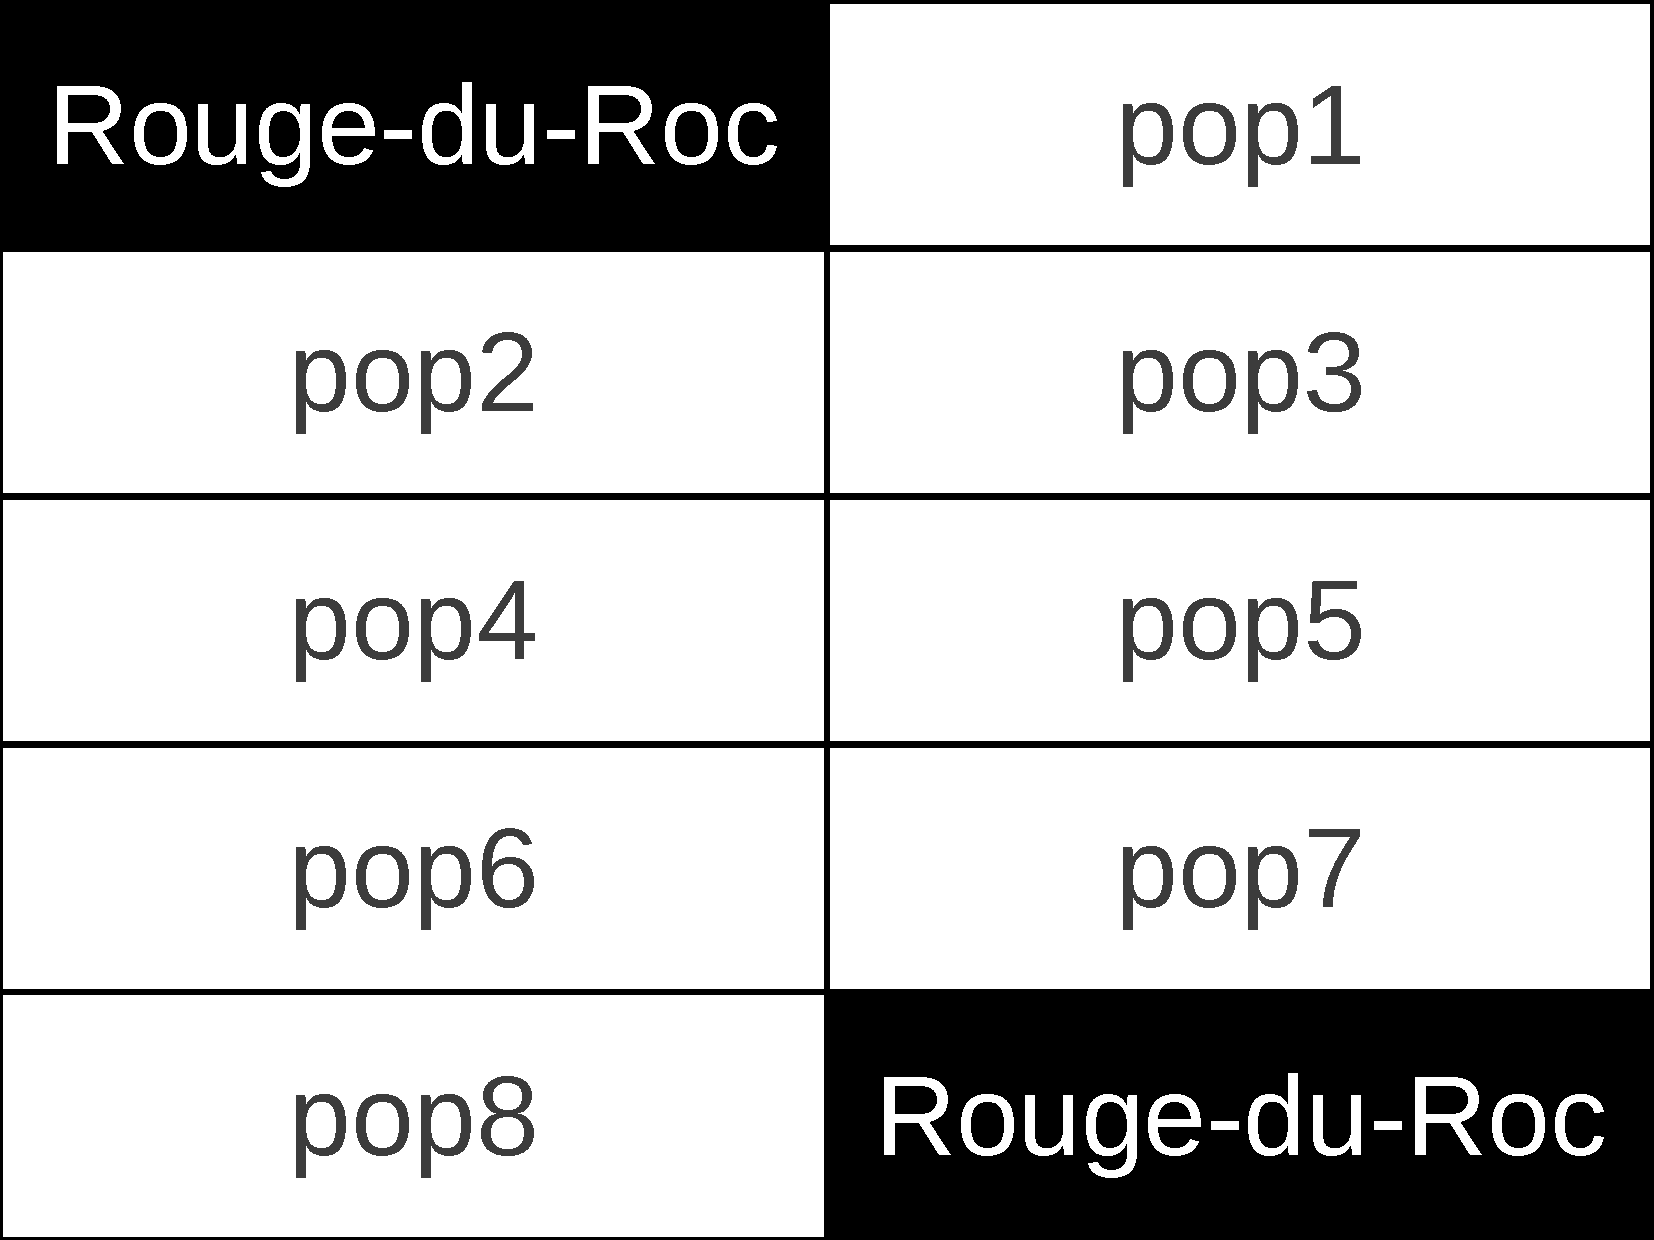
\includegraphics[width=.25\textwidth]{plan_FS.pdf}
                        &
                        \vspace{.5cm}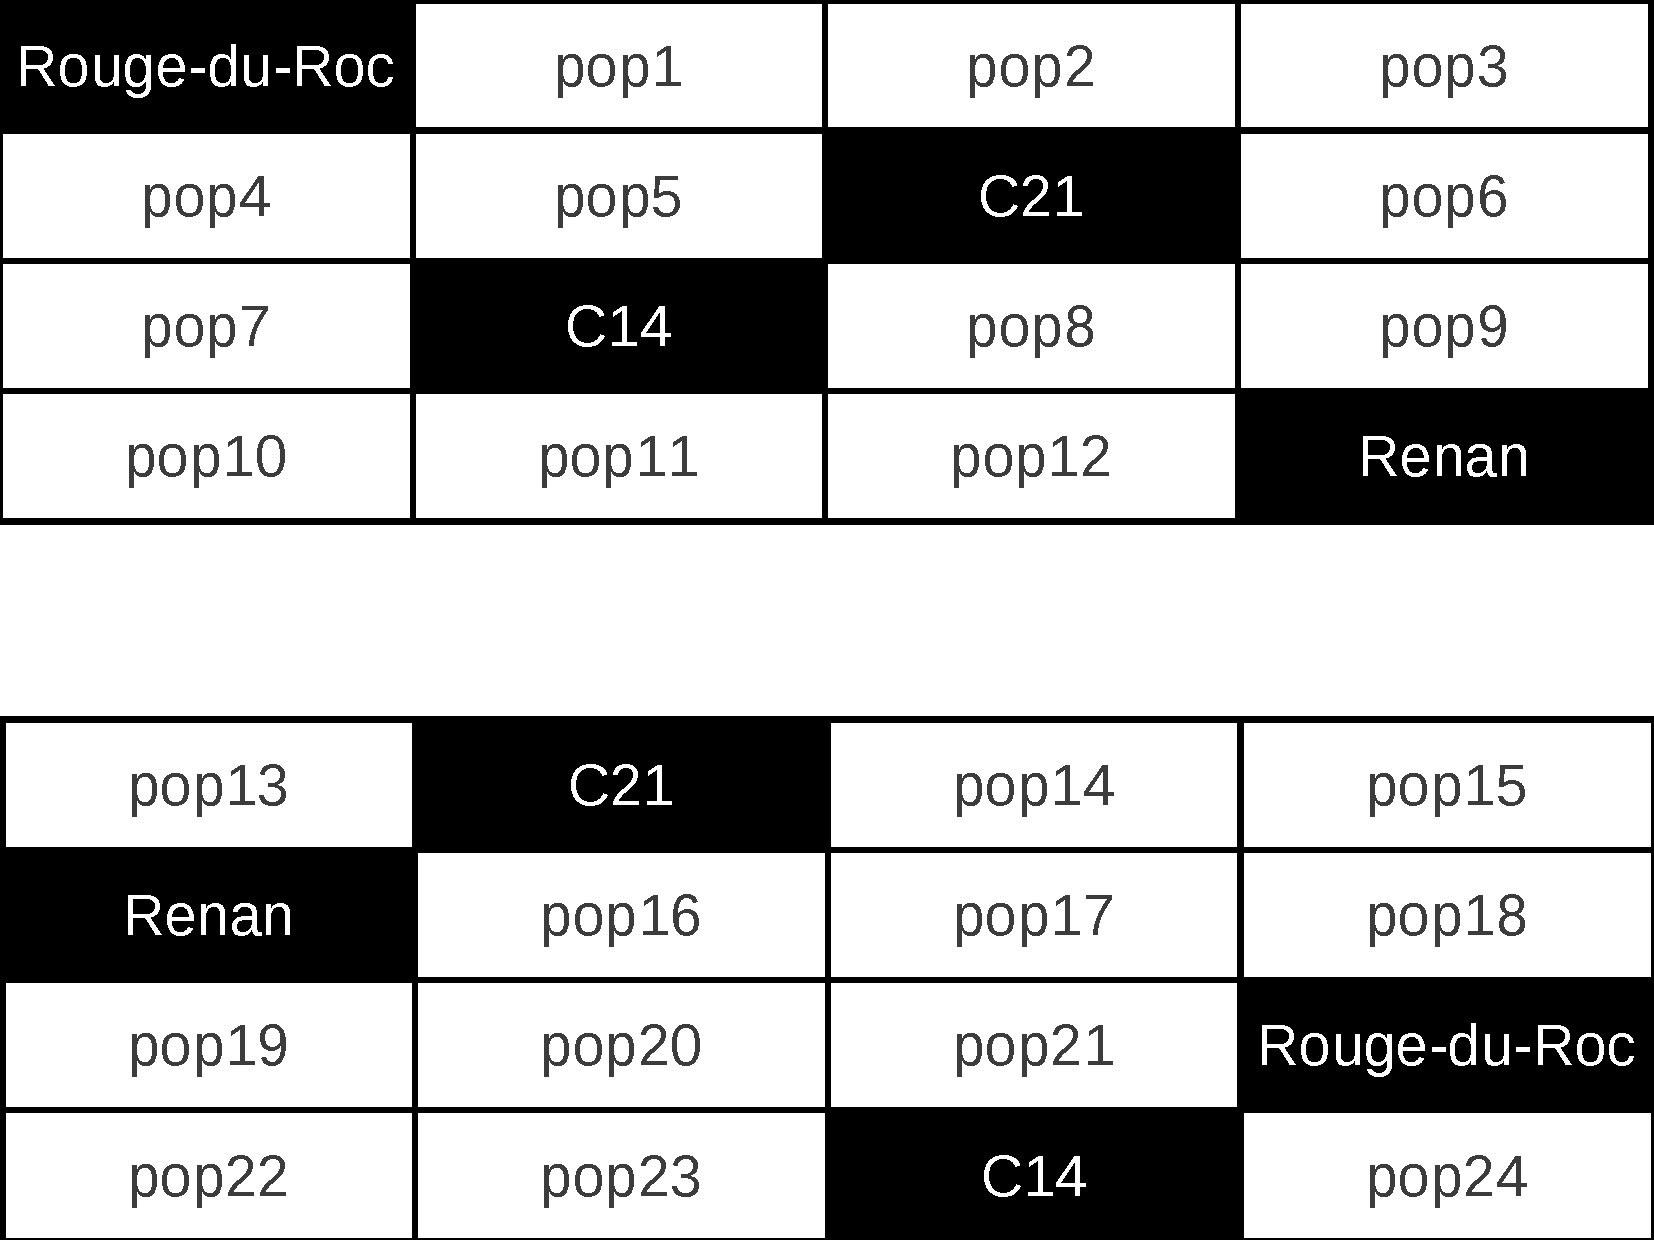
\includegraphics[width=.45\textwidth]{plan_FR.pdf} \\
                        satellite farm & regional farm \\
                        \hline
                \end{tabular}

                \caption{Experimental design of satellite and regional farms. Controls replicated are in black boxes : $Rouge$-$du$-$Roc$, $Renan$, $C14$ and $C21$. pop stands for `tested population'.}
                \label{plan_SF_RF}
        \end{center}
\end{figure}

\begin{itemize}
\item At the \textbf{farm level}, the residual had few degrees of freedom, leading to a poor estimation of the residual variance and to a lack of power for comparing populations.
Hence, model~\ref{model1} was implemented (section~\ref{section_model1}).

\item At the \textbf{network level}, there is a large germplasm $\times$ environment combinaisons that are missing, leading to a poor estimation of germplasm, environment and interaction effects.
Hence, model~\ref{model2} was implemented (section~\ref{section_model2}).

\end{itemize}

These methods are of interest if you have a large data set with a high number of environments and germplasms.
For model \ref{model1}, it gave nice results with more than 20 environment \citep{riviere_hierarchical_2015}.
For model \ref{model2}, it gave nice results with 75 environments and 120 germplasms present in at least two environments (95\% of missing $G \times E$ combinaisons) \citep{riviere_hierarchical_2015-1}.

This will be further explore in simulation studies.

\subsection{Function relations in \pack}

\pack~is divided into two sets of functions:


\begin{itemize}
\item Hidden functions
\item Used functions
\end{itemize}


In this vignette, we only used examples with used functions.
Nevertheless, hidden functions could be used in other context to answer specific questions.
Figure~\ref{function_relations} displays these functions and their relations.
Table~\ref{function_descriptions} gives a quick description of each function.
You can have more information for each function by typing \texttt{?function\_name} in your \R~session.


\begin{figure}[H]
\begin{center}
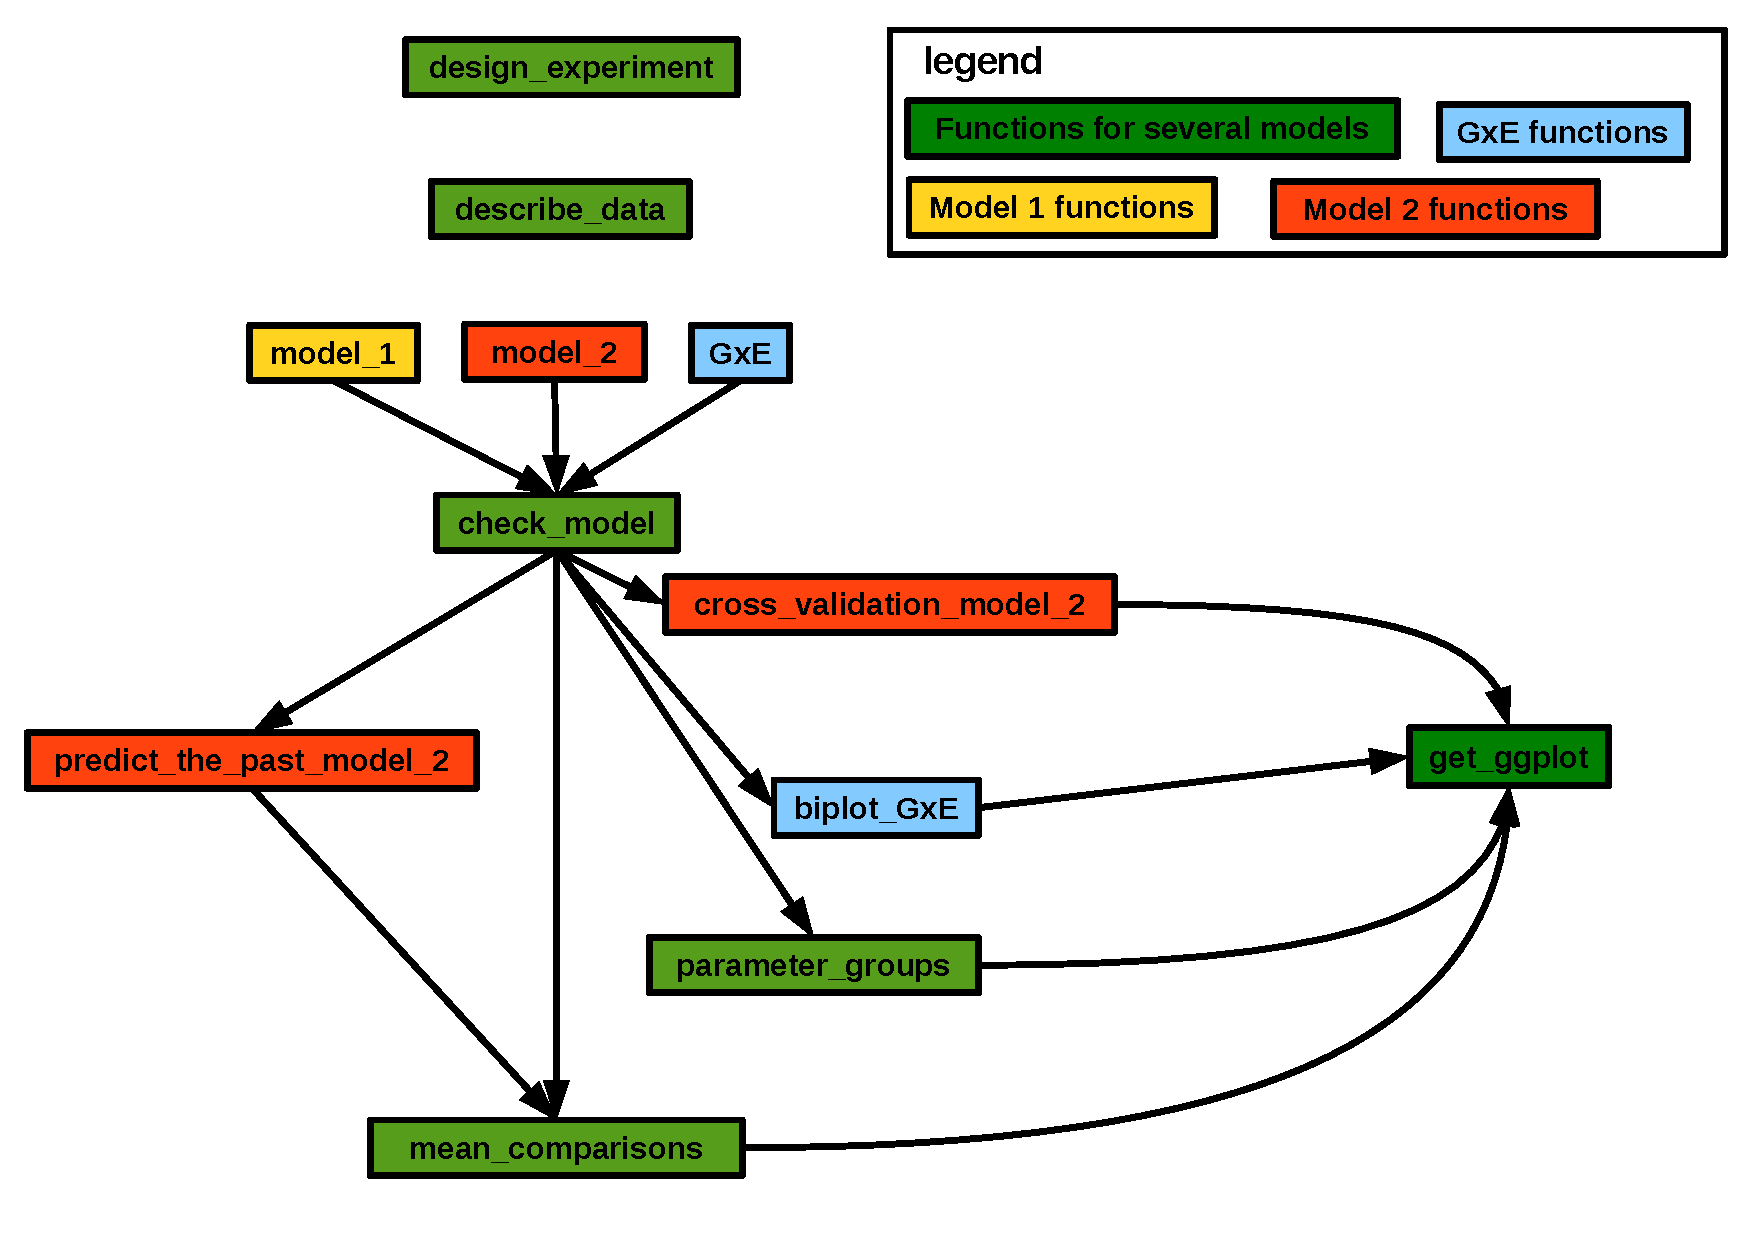
\includegraphics[width=\textwidth]{PBBstats_function_relations}
\end{center}
\caption{Function relations in \pack.
Functions related to model \ref{model1} are in red.
Functions related to model \ref{model2} are in orange.
Functions related to both models are in black.
}
\label{function_relations}
\end{figure}

\begin{table}[t]
\begin{tabular}{cp{.6\textwidth}}

\hline
\textbf{function name} & \textbf{description} \\

\hline
\hline

\texttt{MC} & Run model~\ref{model1} to get mean comparisons (MC) on each environment of the network.\\
\hline

\texttt{FWH} & Run model~\ref{model2} to get main germplasm, environment and sensitivity effects over the network. \\
\hline

\texttt{analyse.outputs} & Check with plots if the model went well based ont the Gelman-Rubin test and plots of posteriors distributions (see section \ref{section_bayes}). It is important to run this step before going ahead in the analysis otherwise you may make mistakes in the interpretation of the results \\
\hline

\texttt{get.mean.comparisons} & Get mean comparisons for a given parameter two by two or to a given threshold based on MCMC outputs \\
\hline

\texttt{get.parameter.groups} & Get groups of parameters based on multivariate analysis \\
\hline

\texttt{cross.validation.FWH} & Run complete cross vlidation with model~\ref{model2} \\
\hline

\texttt{predict.the.past} & Estimate value of a germplasm in an environment based on the FWH model. \\
\hline

\texttt{get.ggplot} & Get ggplot objects to visualize output from the analysis \\
\hline

\hline


\texttt{get.env.info} & Get regional farms data and satellite farms data \\
\hline

\texttt{comp.parameters} & Get parameter comparisons two by two or to a given threshold based on MCMC outputs \\
\hline

\texttt{get.significant.groups} & Get significant groups of differences for a set of parameters based on MCMC outputs \\
\hline

\texttt{get.at.least.X.groups} & Get the value of type one error needed to have X groups. \\
\hline


\end{tabular}
\caption{Function descriptions in \pack.}
\label{function_descriptions}
\end{table}




\subsection{Bayesian statistics}
\label{section_bayes}

The analyses performed in \pack~are based on Bayesian statistics.

Bayesian statistics are based on the Bayes theorem:

\begin{displaymath}
Pr(\theta|y) \propto Pr(\theta) Pr(y|\theta)
\end{displaymath}

with 
$Pr(\theta|y)$ the posterior, 
$Pr(y|\theta)$ the likelihood and 
$Pr(\theta)$ the prior.

The parameters' distribution, knowing the data (the posterior), is proportional to the distribution \textit{a  priori} (the prior) $\times$ the information brought by the data (the likelihood).

The more information (i.e. the larger the data set and the better the model fits the data), the less the prior would be of importance.
If the priors equal the posteriors, it means that there is not enough data or the model does not fit the data.


Bayesian inference is based on the posterior distribution of model parameters.
This distribution could not be calculated explicitely for the hierarchical model used in here (see section~\ref{section_model1} and section~\ref{section_model2}) but could be estimated using Markov Chain and Monte Carlo (MCMC) methods.

These methods simulate values of model parameters according to a Markov chain that converges to the posterior distribution of model parameters \citep{robert_bayesian_2001}.

MCMC methods were implemented using \texttt{JAGS} by the \texttt{R} package \texttt{rjags} that performed Gibbs sampling \citep{robert_bayesian_2001}.
Two MCMC chains were run independently to test for convergence using the Gelman-Rubin test.
This test was based on the variance within and between the chains \citep{gelman_inference_1992}.

A burn-in and lots of iterations were needed in the MCMC procedure.
In our case, the burn-in had 1000 iterations, then 100 000 iterations are done by default\footnote{You can change it with the argument \texttt{nb\_iterations} in functions \texttt{MC} and \texttt{FWH}} with a thinning interval of 10 to reduce autocorrelations between samples, so that 10 000 samples were available for inference for each chain by default\footnote{There are \texttt{nb\_iterations}/10 values for each chain. This can be changed with the \texttt{thin} argument of the functions.}.
 
The final distribution of a posterior is the concatenation of the two MCMC chains: 20 000 samples.



\subsection{Let's go!}
To continue, load the package:
\begin{knitrout}
\definecolor{shadecolor}{rgb}{0.969, 0.969, 0.969}\color{fgcolor}\begin{kframe}
\begin{alltt}
\hlkwd{library}\hlstd{(PPBstats)}
\end{alltt}
\end{kframe}
\end{knitrout}
and download from internet the data used in this vignette (this is useful to earn lots of time!) here : \url{https://www.dropbox.com/sh/6qvl515k5484zg4/AADZKkaM2XZvmr9e6l5aWxN2a?dl=0} and put it in the folder \texttt{data\_PPBstats} and then load() it.

%The example in this vignette were performed with a computer with 4 Gb of memory and the following processor : Intel(R) Core(TM) i5-4210M CPU @ 2.60GHz.
%This gives an idea about memory and processor needed to run the analysis.

\section{At the farm level : model~\ref{model1} to perform mean comparisons on farms }
\label{section_model1}

\subsection{The model}
We restricted ourselves to analysing plot means.
The phenotypic value $Y_{ijk}$ for variable $Y$, germplasm $i$, environment $j$ and block $k$ was modelled as :

\begin{equation}
	Y_{ijk} = \mu_{ij} + \beta_{jk} + \varepsilon_{ijk} ; \quad \varepsilon_{ijk} \sim \mathcal{N} (0,\sigma^2_{j}),
	\label{model1}
\end{equation}

where
$\mu_{ij}$ was the mean of germplasm $i$ in environment $j$ (note that this parameter, which corresponds to an entry, confounds the population effect and the population $\times$ environment effect);
$\beta_{jk}$ was the effect of block $k$ in environment $j$ satisfying the constraint\footnote{Note that it is quite different from \citet{riviere_hierarchical_2015} where the model was done only for two blocks. Here there is no restriction on the number of blocks.} $\sum\limits_{k=1}^K \beta_{jk} = 1$ ;
$\varepsilon_{ijk}$ was the residual error;
$\mathcal{N} (0,\sigma^2_{j})$ denoted normal distribution centred on 0 with variance $\sigma^2_{j}$, which was specific to environment $j$.

We took advantage of the similar structure of the trials on each environment of the network to assume that trial residual variances came from a common distribution :

\begin{displaymath}
	\sigma^2_{j} \sim \frac{1}{Gamma(\nu,\rho)},
\end{displaymath}

where $\nu$ and $\rho$ are unknown parameters.
Because of the low number of residual degrees of freedom for each farm, we used a hierarchical approach in order to assess mean differences on farm.
For that, we placed vague prior distributions on the hyperparameters $\nu$ and $\rho$ :

\begin{displaymath}
	\nu \sim Uniform(\nu_{min},\nu_{max}) ; \quad \rho \sim Gamma(10^{-6},10^{-6}).
\end{displaymath}


In other words, the residual variance of a trial within environment was estimated using all the informations available on the network rather than using the data from that particular trial only.

The parameters $\mu_{ij}$ and $\beta_{j1}$ were assumed to follow vague prior distributions~:

\begin{displaymath}
	\mu_{ij} \sim \mathcal{N}(\mu_{.j},10^{6}); \quad \beta_{j1} \sim \mathcal{N}(0,10^{6}).
\end{displaymath}


The inverse gamma distribution has a support bounded by 0 (consistent with the definition of a variance) and may have various shapes including asymmetric distributions.
From an agronomical point of view, the assumption that trial variances were heterogeneous was consistent with organic farming: there were as many environments as farmers leading to a high heterogeneity.
Environment was here considered in a broad sense: practices (sowing date, sowing density, tilling, etc.), pedo climatic conditions, biotic and abiotic stress, \dots \citep{desclaux_changes_2008}.
Moreover, the inverse gamma distribution had conjugate properties that facilitated MCMC convergence.
This model was therefore a good choice based on both agronomic and statistical criteria.

The residual variance estimated from the controls was assumed to be representative of the residual variance of the other entries.
Blocks were included in the model only if the trial had blocks.





\subsection{With \pack}

For model~\ref{model1}, you can follow these steps (Figure \ref{function_relations}):

\begin{enumerate}
\item Run the model with \texttt{MC}
\item Analyse model outputs with graphs to know if you can continue the analysis with \texttt{analyse.outputs}
\item Get mean comparisons for each factor with \texttt{get.mean.comparisons} and \texttt{get.ggplot}
\end{enumerate}



Let's get the data.
The values for $\mu_{ij}$, $\beta_{jk}$, $\epsilon_{ijk}$ and $\sigma_j$ are the real value taken to create the dataset.
This dataset is representative of data you can get in a PPB programme.

\begin{knitrout}
\definecolor{shadecolor}{rgb}{0.969, 0.969, 0.969}\color{fgcolor}\begin{kframe}
\begin{alltt}
\hlkwd{data}\hlstd{(PPBdata)}
\hlkwd{head}\hlstd{(PPBdata)}
\end{alltt}
\begin{verbatim}
##   year location germplasm block X Y      tkw    mu_ij beta_jk
## 1 2010   env1-1     tem-1     1 1 a 72.09900 73.37224       0
## 2 2010   env1-1     tem-2     1 2 b 61.05274 61.61823       0
## 3 2010   env1-1     tem-3     1 3 c 62.99350 64.31830       0
## 4 2010   env1-1     tem-4     1 4 d 65.10909 62.57840       0
## 5 2010   env1-1     tem-1     2 5 e 77.01361 73.37224       0
## 6 2010   env1-1     tem-2     2 6 f 64.10541 61.61823       0
##   epsilon_ijk  sigma_j
## 1  -1.2732421 1.622339
## 2  -0.5654918 1.622339
## 3  -1.3248006 1.622339
## 4   2.5306946 1.622339
## 5   3.6413666 1.622339
## 6   2.4871807 1.622339
\end{verbatim}
\end{kframe}
\end{knitrout}

\subsubsection{Run the model}

To run model~\ref{model1} on the dataset, used the function \texttt{MC}.
You can run it on one variable.
Here it is thousand kernel weight (tkw).

By default, \texttt{MC} returns posteriors for 
$\mu_{ij}$ (\texttt{return.mu = TRUE}), 
$\beta_{jk}$ (\texttt{return.beta = TRUE}), 
$\sigma_j$ (\texttt{return.sigma = TRUE}), 
$\nu$ (\texttt{return.nu = TRUE}) and 
$\rho$ (\texttt{return.rho = TRUE}).
You can also get $\epsilon_{ijk}$ value with \texttt{return.espilon = TRUE}.

By default, DIC is not displayed, you may want this value to compare to other model (\texttt{DIC = TRUE}).
DIC criterion is a generalization of the AIC criterion that can be used for hierarchical models \citep{spiegelhalter_bayesian_2002}.
The smaller the DIC value, the better the model \citep{plummer_penalized_2008}.

\begin{knitrout}
\definecolor{shadecolor}{rgb}{0.969, 0.969, 0.969}\color{fgcolor}\begin{kframe}
\begin{alltt}
\hlcom{# out.model1 = MC(data = PPBdata, variable = "tkw", return.epsilon = TRUE)}
\hlcom{#Compiling model graph}
\hlcom{#   Resolving undeclared variables}
\hlcom{#   Allocating nodes}
\hlcom{#   Graph Size: 7662}
\hlcom{#}
\hlcom{#Initializing model}
\hlcom{#}
\hlcom{#  |++++++++++++++++++++++++++++++++++++++++++++++++++| 100%}
\hlcom{#  |**************************************************| 100%}
\hlcom{#  |**************************************************| 100%}
\hlcom{#  |**************************************************| 100%}

\hlkwd{load}\hlstd{(}\hlstr{"./data_PPBstats/out.model1.RData"}\hlstd{)} \hlcom{# To save time}
\end{alltt}
\end{kframe}
\end{knitrout}

You can get informations of the environments in the dataset :

\begin{knitrout}
\definecolor{shadecolor}{rgb}{0.969, 0.969, 0.969}\color{fgcolor}\begin{kframe}
\begin{alltt}
\hlstd{out.model1}\hlopt{$}\hlstd{vec_env_with_no_data}
\end{alltt}
\begin{verbatim}
## [1] "env4:2011"
\end{verbatim}
\begin{alltt}
\hlstd{out.model1}\hlopt{$}\hlstd{vec_env_with_no_controls}
\end{alltt}
\begin{verbatim}
## [1] "env5:2010"
\end{verbatim}
\begin{alltt}
\hlstd{out.model1}\hlopt{$}\hlstd{vec_env_with_controls}
\end{alltt}
\begin{verbatim}
##  [1] "env1-1:2010"  "env1-1:2011"  "env1-1:2012"  "env1-2:2010" 
##  [5] "env1-2:2011"  "env1-2:2012"  "env1-3:2010"  "env1-3:2011" 
##  [9] "env1-3:2012"  "env1-4:2010"  "env1-4:2011"  "env1-4:2012" 
## [13] "env1-5:2011"  "env2-10:2010" "env2-10:2011" "env2-10:2012"
## [17] "env2-11:2011" "env2-11:2012" "env2-1:2010"  "env2-1:2011" 
## [21] "env2-1:2012"  "env2-12:2011" "env2-12:2012" "env2-13:2011"
## [25] "env2-13:2012" "env2-14:2011" "env2-14:2012" "env2-15:2011"
## [29] "env2-15:2012" "env2-2:2010"  "env2-2:2011"  "env2-2:2012" 
## [33] "env2-3:2010"  "env2-3:2011"  "env2-3:2012"  "env2-4:2010" 
## [37] "env2-4:2011"  "env2-4:2012"  "env2-5:2010"  "env2-5:2011" 
## [41] "env2-5:2012"  "env2-6:2010"  "env2-6:2011"  "env2-6:2012" 
## [45] "env2-7:2010"  "env2-7:2011"  "env2-7:2012"  "env2-8:2010" 
## [49] "env2-8:2011"  "env2-8:2012"  "env2-9:2010"  "env2-9:2011" 
## [53] "env2-9:2012"  "env3-1:2011"  "env3-1:2012"  "env3-2:2011" 
## [57] "env3-2:2012"  "env3-3:2011"
\end{verbatim}
\begin{alltt}
\hlstd{out.model1}\hlopt{$}\hlstd{vec_env_RF}
\end{alltt}
\begin{verbatim}
##  [1] "env1-1:2010" "env1-1:2011" "env1-1:2012" "env1-2:2010"
##  [5] "env1-2:2011" "env1-2:2012" "env1-3:2010" "env1-3:2011"
##  [9] "env1-3:2012" "env1-4:2010" "env1-4:2011" "env1-4:2012"
## [13] "env1-5:2011" "env3-1:2011" "env3-1:2012" "env3-2:2011"
## [17] "env3-2:2012" "env3-3:2011"
\end{verbatim}
\begin{alltt}
\hlstd{out.model1}\hlopt{$}\hlstd{vec_env_SF}
\end{alltt}
\begin{verbatim}
##  [1] "env2-10:2010" "env2-10:2011" "env2-10:2012" "env2-11:2011"
##  [5] "env2-11:2012" "env2-1:2010"  "env2-1:2011"  "env2-1:2012" 
##  [9] "env2-12:2011" "env2-12:2012" "env2-13:2011" "env2-13:2012"
## [13] "env2-14:2011" "env2-14:2012" "env2-15:2011" "env2-15:2012"
## [17] "env2-2:2010"  "env2-2:2011"  "env2-2:2012"  "env2-3:2010" 
## [21] "env2-3:2011"  "env2-3:2012"  "env2-4:2010"  "env2-4:2011" 
## [25] "env2-4:2012"  "env2-5:2010"  "env2-5:2011"  "env2-5:2012" 
## [29] "env2-6:2010"  "env2-6:2011"  "env2-6:2012"  "env2-7:2010" 
## [33] "env2-7:2011"  "env2-7:2012"  "env2-8:2010"  "env2-8:2011" 
## [37] "env2-8:2012"  "env2-9:2010"  "env2-9:2011"  "env2-9:2012"
\end{verbatim}
\end{kframe}
\end{knitrout}

\subsubsection{Analysis of the model outputs}
Once the model is run, it is necessary to check if the outputs can be taken with confidence.
This step is needed before going ahead in the analysis (in fact, the MCMC object used in the next functions must come from \texttt{analyse.outputs}!).

\begin{knitrout}
\definecolor{shadecolor}{rgb}{0.969, 0.969, 0.969}\color{fgcolor}\begin{kframe}
\begin{alltt}
\hlcom{# The experimental design plot is done.}
\hlcom{# The Gelman-Rubin test is running for each parameter ...}
\hlcom{# The two MCMC for each parameter converge thanks to the Gelman-Rubin test.}
\hlcom{# The values of sigma in the inverse Gamme distribution are done.}
\hlcom{# The mu_ij posterior distributions are done.}
\hlcom{# The beta_jk posterior distributions are done.}
\hlcom{# The sigma_j posterior distributions are done.}
\hlcom{# The standardised residuals distributions are done.}

\hlkwd{load}\hlstd{(}\hlstr{"./data_PPBstats/out1.RData"}\hlstd{)}
\end{alltt}
\end{kframe}
\end{knitrout}

\texttt{out1} is a list containing:

\begin{itemize}

\item "experimental\_design" : a plot representing the presence/abscence matrix of G $\times$ E combinaisons. 
Here there are lots of 0 meaning that a lot of germplasm are no in at least two farms.
A score of 1 is for a given germplasm in a given environment.
A score of 2 is for a given germplasm replicated twice in a given environement.
A score of 3 is for a given germplasm replicated three times in a given environement.

\begin{figure}[H]
\begin{knitrout}
\definecolor{shadecolor}{rgb}{0.969, 0.969, 0.969}\color{fgcolor}\begin{kframe}
\begin{alltt}
\hlstd{out1}\hlopt{$}\hlstd{data.experimental_design}\hlopt{$}\hlstd{plot}
\end{alltt}
\end{kframe}

{\centering 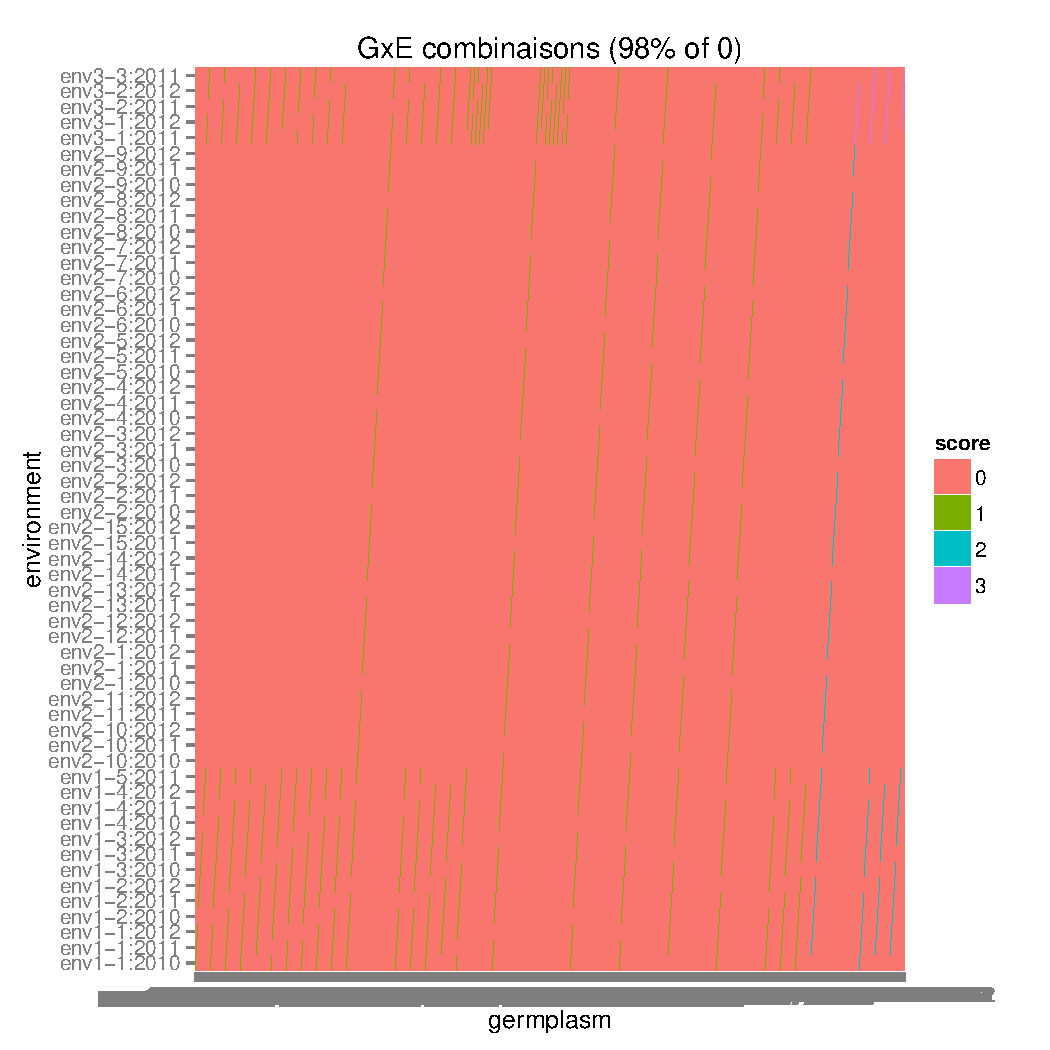
\includegraphics[width=.6\textwidth]{figures/PPBstats_unnamed-chunk-6-1} 

}



\end{knitrout}
\end{figure}

\item "convergence" : a list with the plots of trace and density to check the convergence of the two MCMC only for chains that are not converging thanks to the Gelman-Rubin test \citep{gelman_inference_1992}. If all the chains converge, it is NULL

\begin{figure}[H]
\begin{knitrout}
\definecolor{shadecolor}{rgb}{0.969, 0.969, 0.969}\color{fgcolor}\begin{kframe}
\begin{alltt}
\hlstd{out1}\hlopt{$}\hlstd{convergence}
\end{alltt}
\begin{verbatim}
## NULL
\end{verbatim}
\end{kframe}
\end{knitrout}
\end{figure}

Here all the parameters converge.
Below is an example where there is no convergence because the MCMC are too small.

\begin{figure}[H]
\begin{knitrout}
\definecolor{shadecolor}{rgb}{0.969, 0.969, 0.969}\color{fgcolor}\begin{kframe}
\begin{alltt}
\hlcom{# out.model1_bis = MC(data = PPBdata, variable = "tkw", nb_iteration = 5000)}
\hlcom{#Compiling model graph}
\hlcom{#   Resolving undeclared variables}
\hlcom{#   Allocating nodes}
\hlcom{#   Graph Size: 7662}
\hlcom{#}
\hlcom{#Initializing model}
\hlcom{#}
\hlcom{#  |++++++++++++++++++++++++++++++++++++++++++++++++++| 100%}
\hlcom{#  |**************************************************| 100%}
\hlcom{#  |**************************************************| 100%}
\hlcom{#Warning message:}
\hlcom{#In MC(data = PPBdata, variable = "tkw", nb_iteration = 5000) :}
\hlcom{#  nb_iterations is below 20 000, which seems small to get convergence in the MCMC.}

\hlkwd{load}\hlstd{(}\hlstr{"./data_PPBstats/out.model1_bis.RData"}\hlstd{)} \hlcom{# To save time}

\hlcom{# out1_bis = analyse.outputs(out.model1_bis)}
\hlcom{# The experimental design plot is done.}
\hlcom{# The Gelman-Rubin test is running for each parameter ...}
\hlcom{# The two MCMC of the following parameters do not converge thanks to the Gelman-Rubin test : }
\hlcom{# nu, rho, sigma[env1-1:2012], sigma[env1-2:2011], sigma[env2-12:2012], sigma[env2-6:2010]. }
\hlcom{# Therefore, they are not present in MCMC output.}
\hlcom{# MCMC are updated, the following environment were deleted : }
\hlcom{# env1-1:2012, env1-2:2011, env2-12:2012, env2-6:2010}
\hlcom{# model1.data_env_whose_param_did_not_converge contains the raw data for these environments.}
\hlcom{# The values of sigma in the inverse Gamme distribution are done.}
\hlcom{# The mu_ij posterior distributions are done.}
\hlcom{# The beta_jk posterior distributions are done.}
\hlcom{# The sigma_j posterior distributions are done.}

\hlkwd{load}\hlstd{(}\hlstr{"./data_PPBstats/out1_bis.RData"}\hlstd{)} \hlcom{# To save time}

\hlcom{# Get one example}
\hlstd{toplot} \hlkwb{=} \hlstd{out1_bis}\hlopt{$}\hlstd{convergence}\hlopt{$}\hlstr{"nu"}
\hlkwd{grid.arrange}\hlstd{(toplot}\hlopt{$}\hlstd{traceplot, toplot}\hlopt{$}\hlstd{density,} \hlkwc{ncol}\hlstd{=}\hlnum{2}\hlstd{,} \hlkwc{nrow}\hlstd{=}\hlnum{1}\hlstd{)}
\end{alltt}
\end{kframe}

{\centering 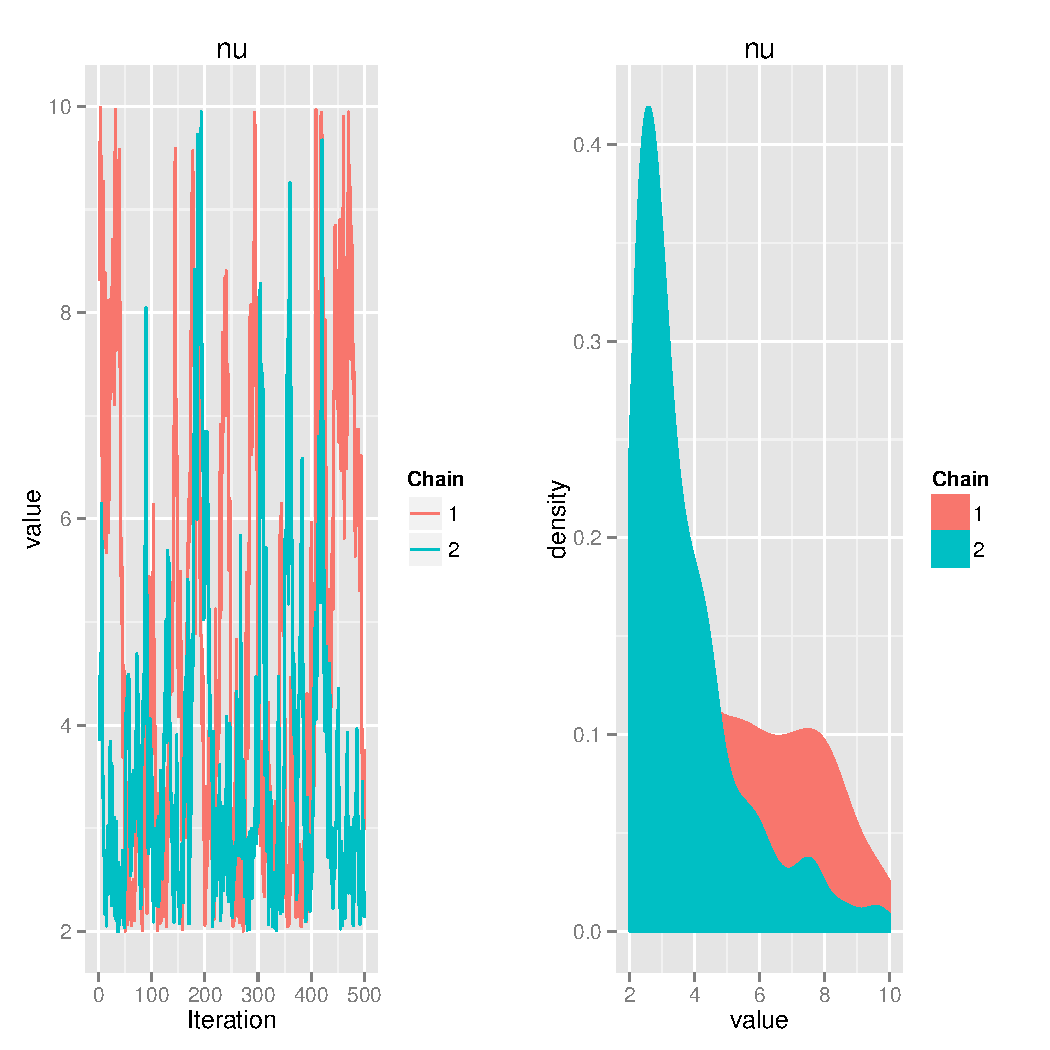
\includegraphics[width=.6\textwidth]{figures/PPBstats_unnamed-chunk-8-1} 

}



\end{knitrout}
\end{figure}


\item "parameter\_posteriors" : a list with

\begin{itemize}

\item "sigma\_distribution" : the distribution of the sigma is displayed on the Inverse Gamma distribution

\begin{figure}[H]
\begin{knitrout}
\definecolor{shadecolor}{rgb}{0.969, 0.969, 0.969}\color{fgcolor}\begin{kframe}
\begin{alltt}
\hlstd{out1}\hlopt{$}\hlstd{posteriors}\hlopt{$}\hlstd{sigma_distribution[[}\hlnum{1}\hlstd{]]} \hlcom{# All the values}
\end{alltt}
\end{kframe}

{\centering 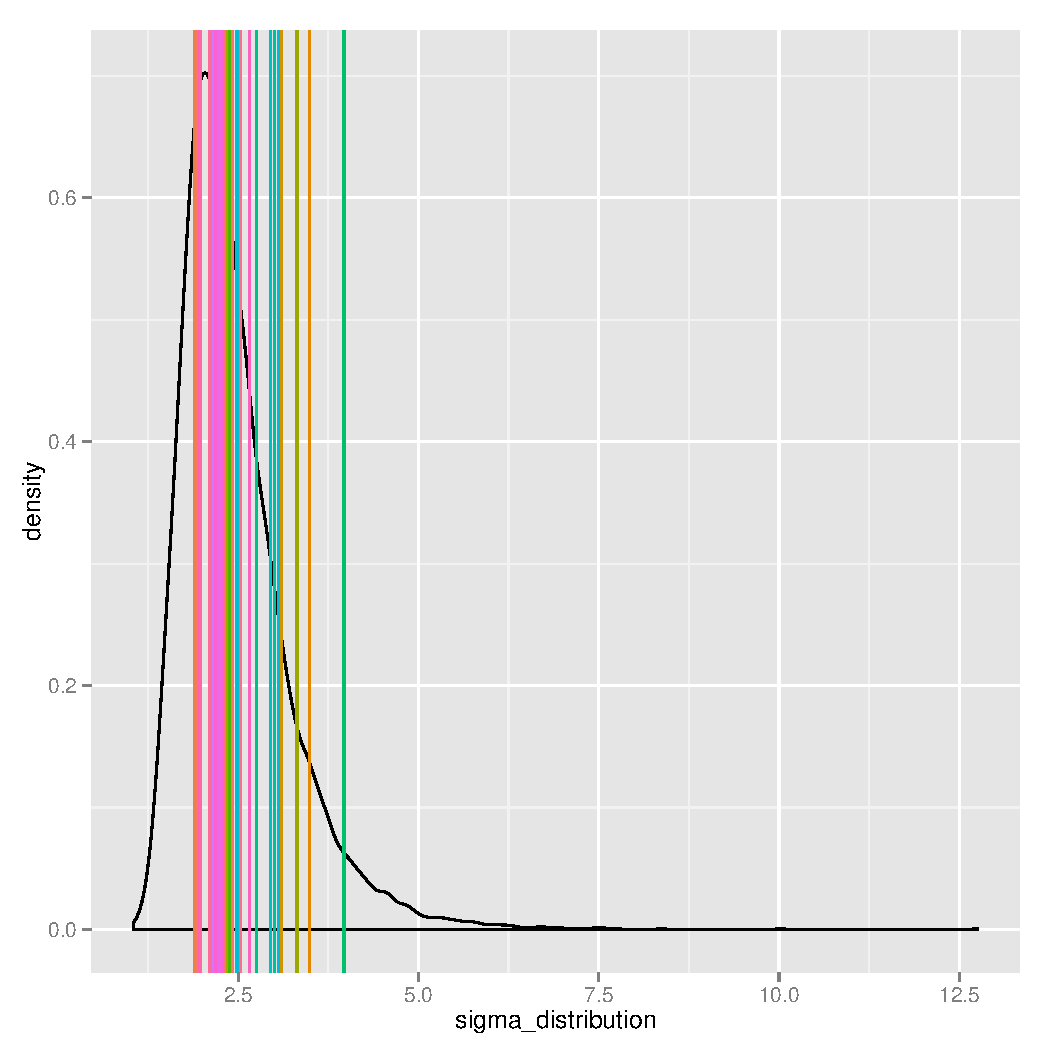
\includegraphics[width=.6\textwidth]{figures/PPBstats_unnamed-chunk-9-1} 

}



\end{knitrout}
\end{figure}


\begin{figure}[H]
\begin{knitrout}
\definecolor{shadecolor}{rgb}{0.969, 0.969, 0.969}\color{fgcolor}\begin{kframe}
\begin{alltt}
\hlstd{out1}\hlopt{$}\hlstd{posteriors}\hlopt{$}\hlstd{sigma_distribution[[}\hlnum{12}\hlstd{]]} \hlcom{# A subset of values}
\end{alltt}
\end{kframe}

{\centering 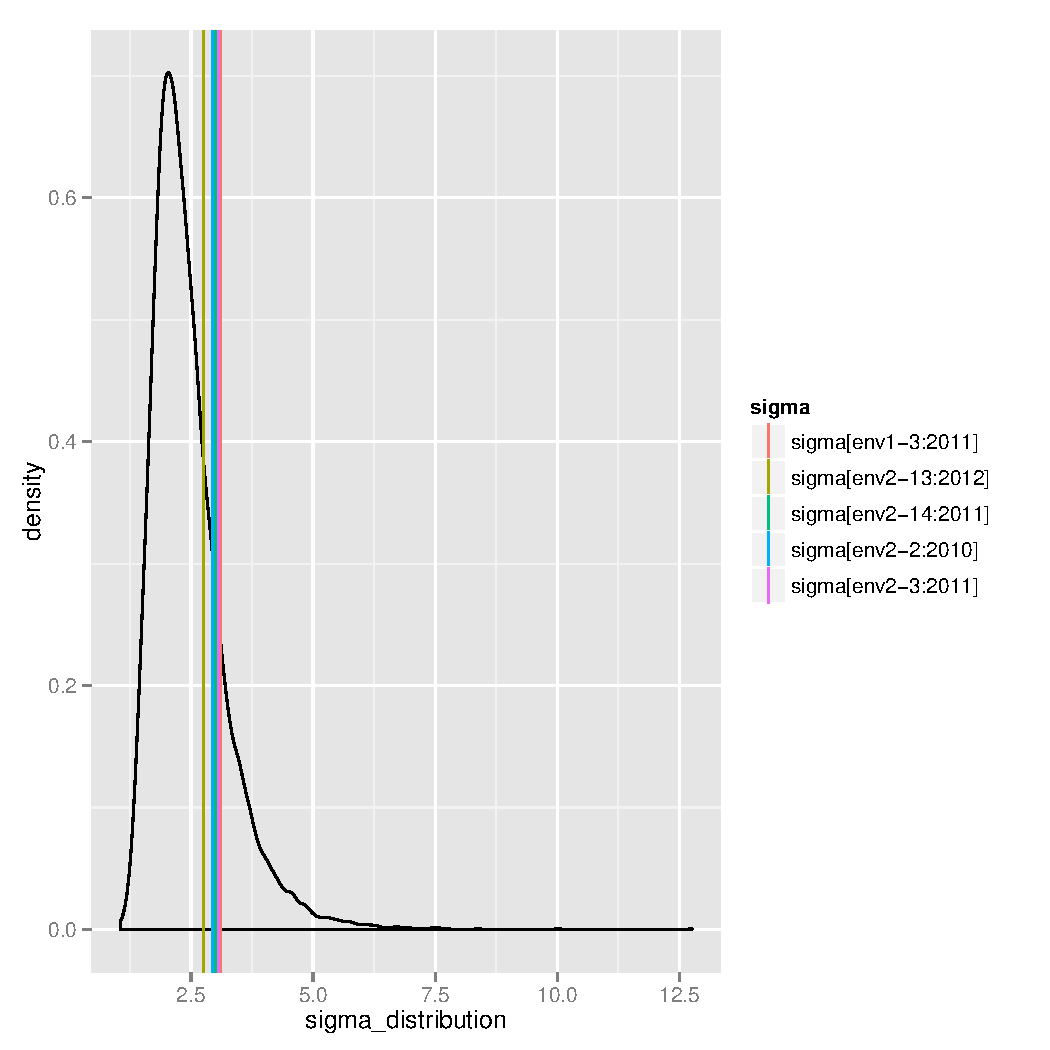
\includegraphics[width=.6\textwidth]{figures/PPBstats_unnamed-chunk-10-1} 

}



\end{knitrout}
\end{figure}


\item "parameter\_posteriors" : a caterpillar plot is display for each $\mu_{ij}$, $\beta_{jk}$ for a each environment and for $\sigma_j$.
Below is an example for environment env1-1:2010.
It is important to see it the values are coherent with your a priori knowledge.
Indeed, a model can converge and estimate parameters'value that are not coherent!

\begin{figure}[H]
\begin{knitrout}
\definecolor{shadecolor}{rgb}{0.969, 0.969, 0.969}\color{fgcolor}\begin{kframe}
\begin{alltt}
\hlstd{out1}\hlopt{$}\hlstd{posteriors}\hlopt{$}\hlstd{parameter_posteriors}\hlopt{$}\hlstd{mu_posteriors}\hlopt{$}\hlstr{"env1-1:2010"}
\end{alltt}
\end{kframe}

{\centering 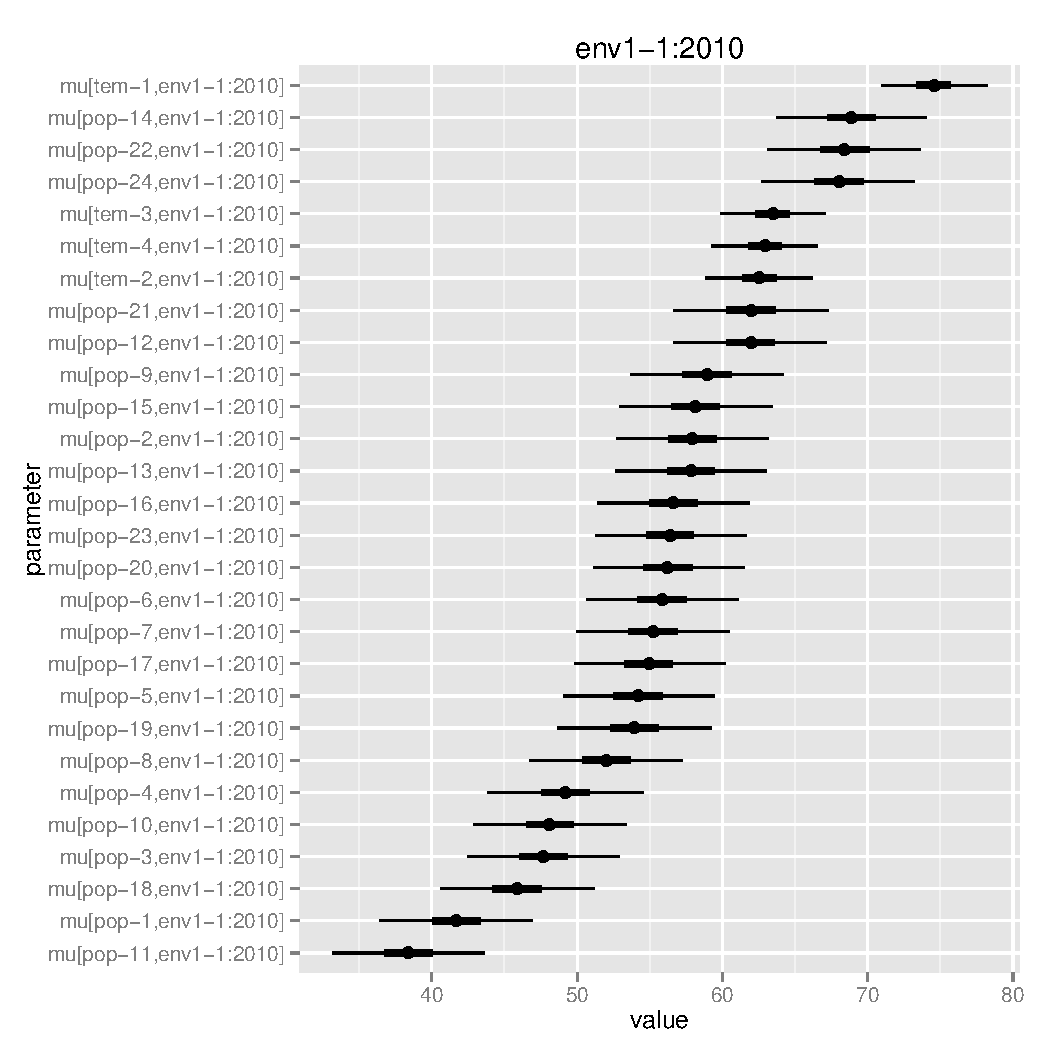
\includegraphics[width=.6\textwidth]{figures/PPBstats_unnamed-chunk-11-1} 

}



\end{knitrout}
\end{figure}

\begin{figure}[H]
\begin{knitrout}
\definecolor{shadecolor}{rgb}{0.969, 0.969, 0.969}\color{fgcolor}\begin{kframe}
\begin{alltt}
\hlstd{out1}\hlopt{$}\hlstd{posteriors}\hlopt{$}\hlstd{parameter_posteriors}\hlopt{$}\hlstd{beta_posteriors}\hlopt{$}\hlstr{"env1-1:2010"}
\end{alltt}
\end{kframe}

{\centering 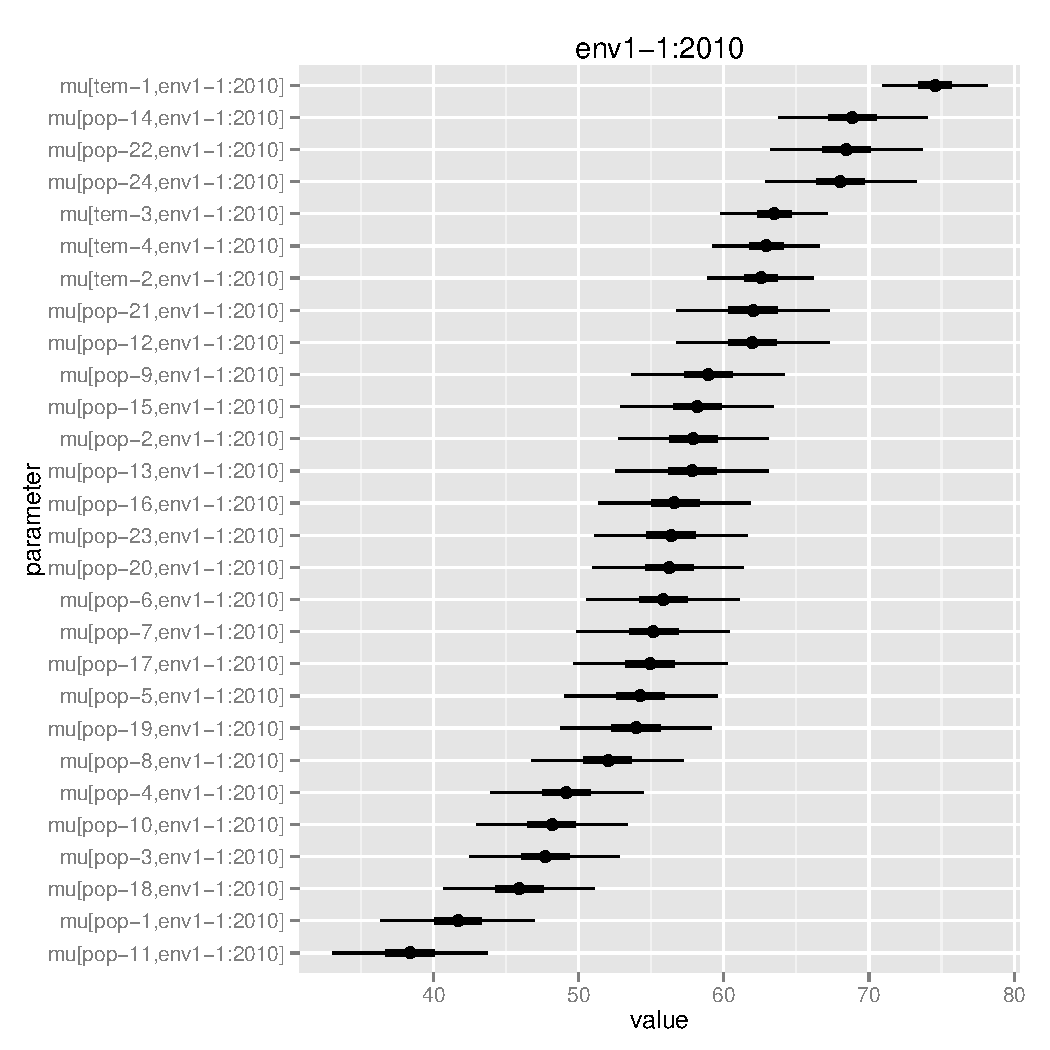
\includegraphics[width=.6\textwidth]{figures/PPBstats_unnamed-chunk-12-1} 

}



\end{knitrout}
\end{figure}

\begin{figure}[H]
\begin{knitrout}
\definecolor{shadecolor}{rgb}{0.969, 0.969, 0.969}\color{fgcolor}\begin{kframe}
\begin{alltt}
\hlstd{out1}\hlopt{$}\hlstd{posteriors}\hlopt{$}\hlstd{parameter_posteriors}\hlopt{$}\hlstd{sigma_posteriors[[}\hlnum{1}\hlstd{]]}
\end{alltt}
\end{kframe}

{\centering 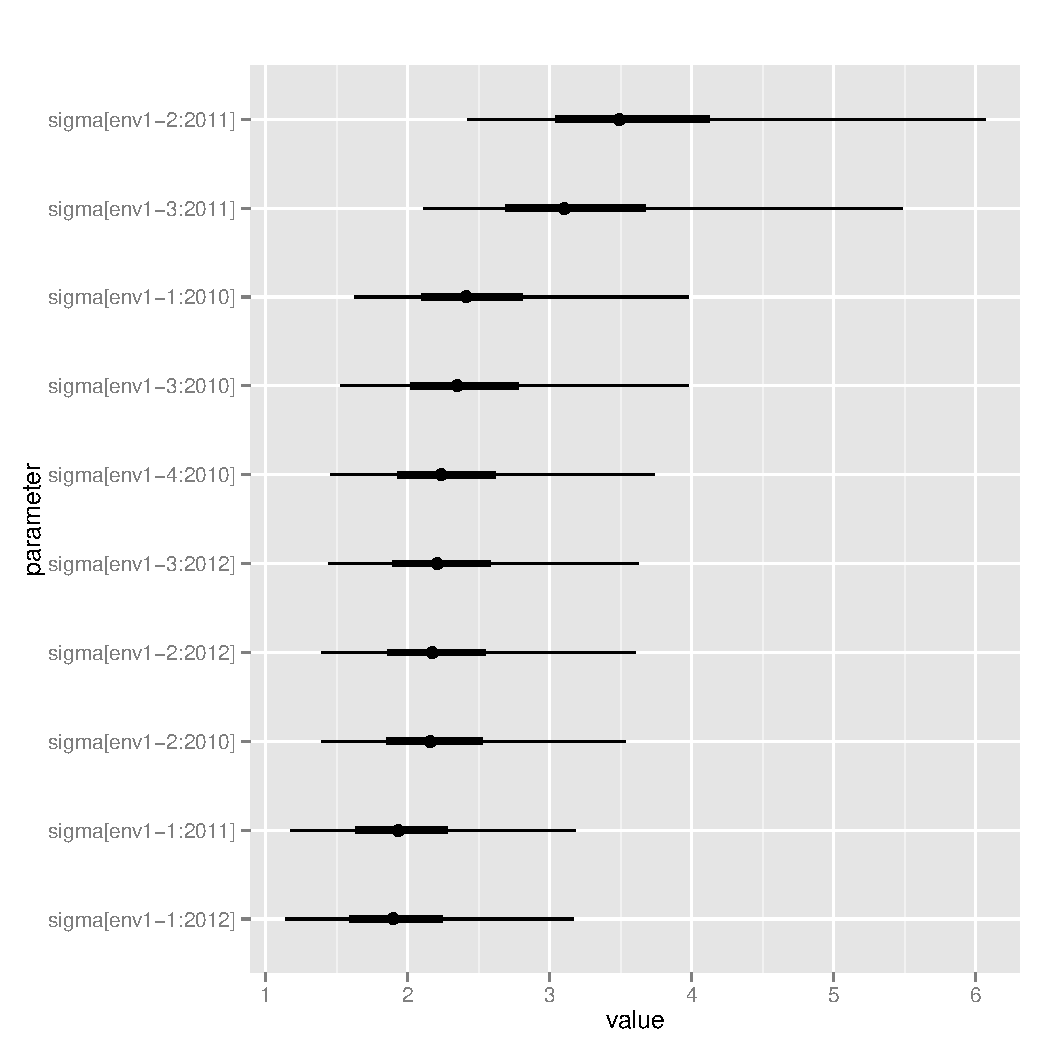
\includegraphics[width=.6\textwidth]{figures/PPBstats_unnamed-chunk-13-1} 

}



\end{knitrout}
\end{figure}

\item "standardized\_residuals" : a plot to check the normality of the residuals. If the model went well it should be between -2 and 2.

\begin{figure}[H]
\begin{knitrout}
\definecolor{shadecolor}{rgb}{0.969, 0.969, 0.969}\color{fgcolor}\begin{kframe}
\begin{alltt}
\hlstd{out1}\hlopt{$}\hlstd{posteriors}\hlopt{$}\hlstd{standardized_residuals}
\end{alltt}
\end{kframe}

{\centering 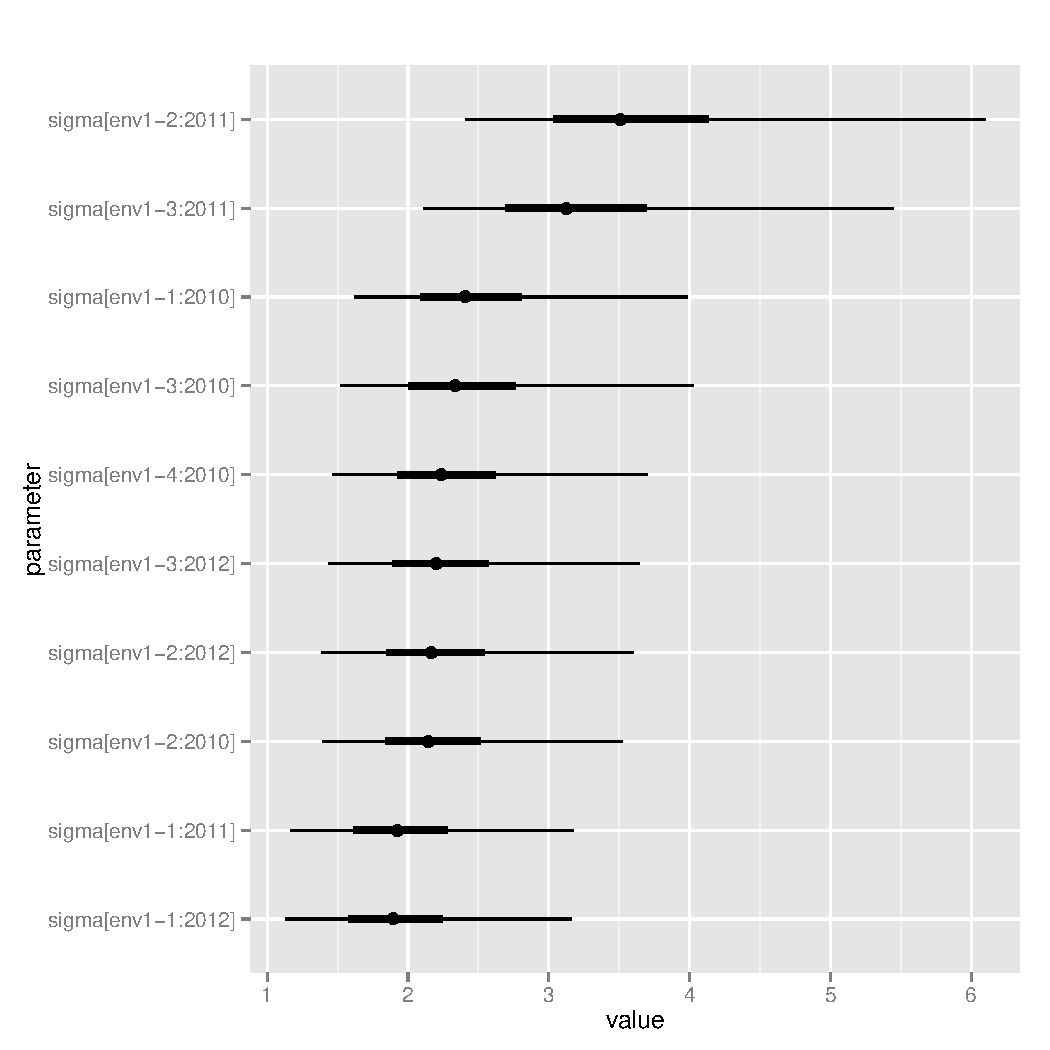
\includegraphics[width=.6\textwidth]{figures/PPBstats_unnamed-chunk-14-1} 

}



\end{knitrout}
\end{figure}

\end{itemize}

\item "MCMC" : a data fame resulting from the concatenation of the two MCMC for each parameter. This object can be used for further analysis. There are as many columns than parameters and as many rows than iterations//thin (the thin value is 10 by default in the models).

\begin{knitrout}
\definecolor{shadecolor}{rgb}{0.969, 0.969, 0.969}\color{fgcolor}\begin{kframe}
\begin{alltt}
\hlkwd{dim}\hlstd{(out1}\hlopt{$}\hlstd{MCMC)}
\end{alltt}
\begin{verbatim}
## [1] 20000   945
\end{verbatim}
\end{kframe}
\end{knitrout}

\end{itemize}

Just for fun, you can compare the posterior medians and the arithmetic means for the $\mu_{ij}$.

\begin{knitrout}
\definecolor{shadecolor}{rgb}{0.969, 0.969, 0.969}\color{fgcolor}\begin{kframe}
\begin{alltt}
\hlstd{MCMC} \hlkwb{=} \hlstd{out1}\hlopt{$}\hlstd{MCMC}
\hlstd{effects} \hlkwb{=} \hlkwd{apply}\hlstd{(MCMC,} \hlnum{2}\hlstd{, median)}
\hlstd{mu_ij_estimated} \hlkwb{=} \hlstd{effects[}\hlkwd{grep}\hlstd{(}\hlstr{"mu"}\hlstd{,}\hlkwd{names}\hlstd{(effects))]}
\hlkwd{names}\hlstd{(mu_ij_estimated)} \hlkwb{=} \hlkwd{sapply}\hlstd{(}\hlkwd{names}\hlstd{(mu_ij_estimated),}
                                \hlkwa{function}\hlstd{(}\hlkwc{x}\hlstd{)\{}  \hlkwd{sub}\hlstd{(}\hlstr{"\textbackslash{}\textbackslash{}]"}\hlstd{,} \hlstr{""}\hlstd{,} \hlkwd{sub}\hlstd{(}\hlstr{"mu\textbackslash{}\textbackslash{}["}\hlstd{,} \hlstr{""}\hlstd{, x)) \}}
                                \hlstd{)}

\hlstd{d} \hlkwb{=} \hlkwd{filter}\hlstd{(PPBdata, location} \hlopt{!=} \hlstr{"env4"}\hlstd{)}
\hlstd{d} \hlkwb{=} \hlkwd{filter}\hlstd{(d, location} \hlopt{!=} \hlstr{"env5"}\hlstd{)}
\hlstd{d} \hlkwb{=} \hlkwd{droplevels}\hlstd{(d)}
\hlstd{environment} \hlkwb{=} \hlkwd{paste}\hlstd{(}\hlkwd{as.character}\hlstd{(d}\hlopt{$}\hlstd{location),} \hlkwd{as.character}\hlstd{(d}\hlopt{$}\hlstd{year),} \hlkwc{sep} \hlstd{=} \hlstr{":"}\hlstd{)}
\hlstd{d}\hlopt{$}\hlstd{entry} \hlkwb{=} \hlkwd{as.factor}\hlstd{(}\hlkwd{paste}\hlstd{(}\hlkwd{as.character}\hlstd{(d}\hlopt{$}\hlstd{germplasm), environment,} \hlkwc{sep} \hlstd{=} \hlstr{","}\hlstd{))}
\hlstd{mu_ij} \hlkwb{=} \hlkwd{tapply}\hlstd{(d}\hlopt{$}\hlstd{mu_ij, d}\hlopt{$}\hlstd{entry, mean,} \hlkwc{na.rm} \hlstd{=} \hlnum{TRUE}\hlstd{)}

\hlstd{check} \hlkwb{=} \hlkwd{cbind.data.frame}\hlstd{(mu_ij, mu_ij_estimated[}\hlkwd{names}\hlstd{(mu_ij)])}
\end{alltt}
\end{kframe}
\end{knitrout}

Let's have a look on the relation between the posterior medians and the arithmetic means.
It goes pretty well!

\begin{figure}[H]
\begin{knitrout}
\definecolor{shadecolor}{rgb}{0.969, 0.969, 0.969}\color{fgcolor}\begin{kframe}
\begin{alltt}
\hlstd{p} \hlkwb{=} \hlkwd{ggplot}\hlstd{(check,} \hlkwd{aes}\hlstd{(}\hlkwc{x} \hlstd{= mu_ij,} \hlkwc{y} \hlstd{= mu_ij_estimated))}
\hlstd{p} \hlopt{+} \hlkwd{stat_smooth}\hlstd{(}\hlkwc{method} \hlstd{=} \hlstr{"lm"}\hlstd{)} \hlopt{+} \hlkwd{geom_point}\hlstd{()}
\end{alltt}
\end{kframe}

{\centering 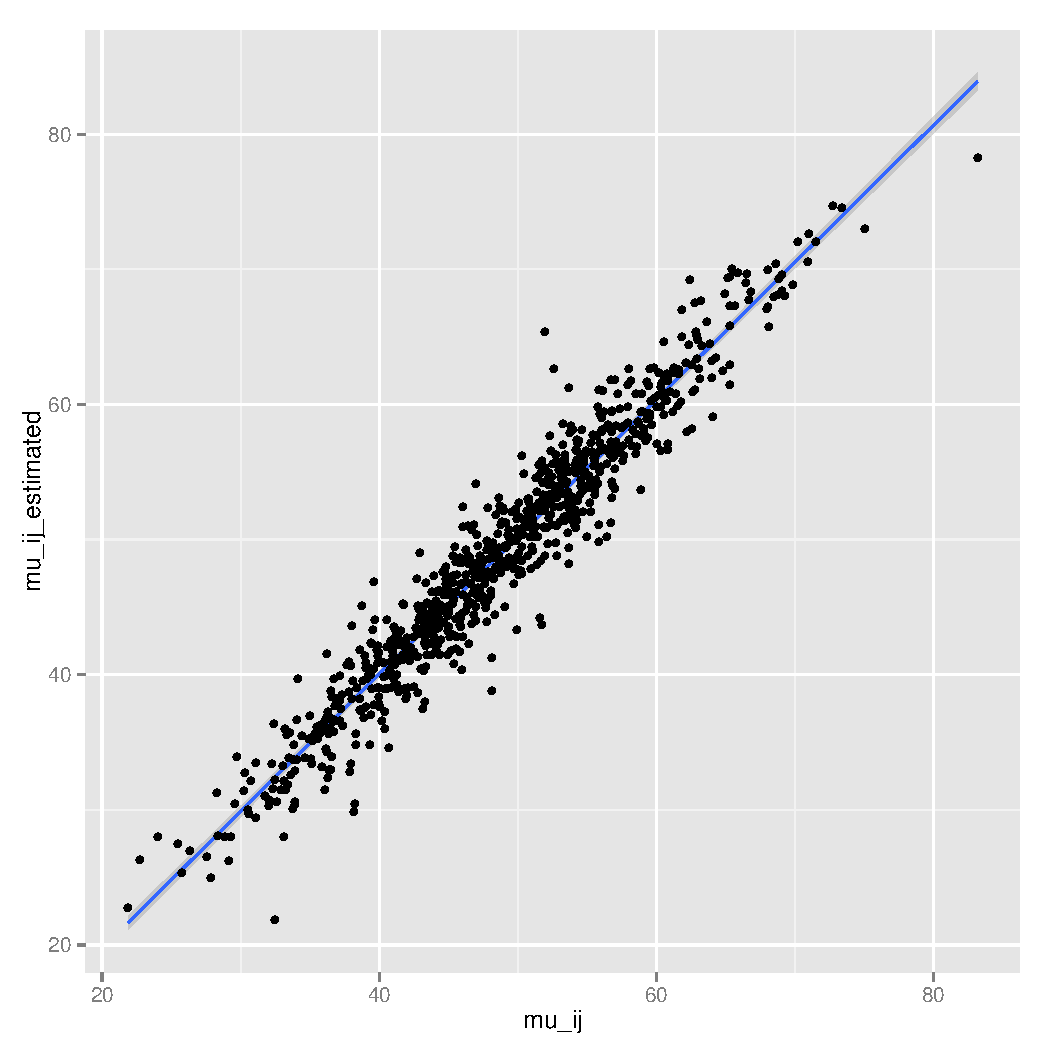
\includegraphics[width=.6\textwidth]{figures/PPBstats_unnamed-chunk-17-1} 

}



\end{knitrout}
\end{figure}


\subsubsection{Get mean comparisons}

\label{mean_comp}
In this part, the mean of each entry is compared to the mean of each other entry.
Let $H_{0}$ and $H_{1}$ denote the hypotheses:

\begin{displaymath}
  H_{0} : \mu_{ij} \ge \mu_{i'j} , \; H_{1} : \mu_{ij} < \mu_{i'j}.
\end{displaymath}

The difference $\mu_{ij}-\mu_{i'j}$ between the means of germplasm $i$ and population $i'$ in environment $j$ was considered as significant if either $H_{0}$ or $H_{1}$ had a high posterior probability, that is if $Pr\{H_{0}|y\} > 1 - \alpha$ or $Pr\{H_{1}|y\}> 1 - \alpha$, where
$\alpha$ was some specified threshold.
The difference was considered as not significant otherwise.
The posterior probability of a hypothesis was estimated by the proportion of MCMC simulations for
which this hypothesis was satisfied (Figure~\ref{proba}).

Groups are made based on the probabilites.
Germplasms which share the same group are not different.
Germplasms which do not share the same groupe are different.

The threshold $\alpha$ that depends on agronomic objectives.
This threshold is set by default to $\alpha=0.1/I$ (with $I$ the number of entries in a given environnement).
It corresponded to a `soft' Bonferroni correction, the Bonferroni correction being very conservative.

As one objective of this PPB programme is that farmers (re)learn selection, the threshold could be adjusted to allow the detection of at least two groups instead of having farmers choose at random.
The initial value could be set to $\alpha=0.1/I$ and if only one group is obtained, then this value could be adjusted to allow the detection of two groups.
In this cases, the farmers should be informed of the lower degree of confidence that there are significant differences among entries.

\begin{figure}[H]
\begin{center}
\begin{pspicture}(10,10)
\rput[bl](0,0){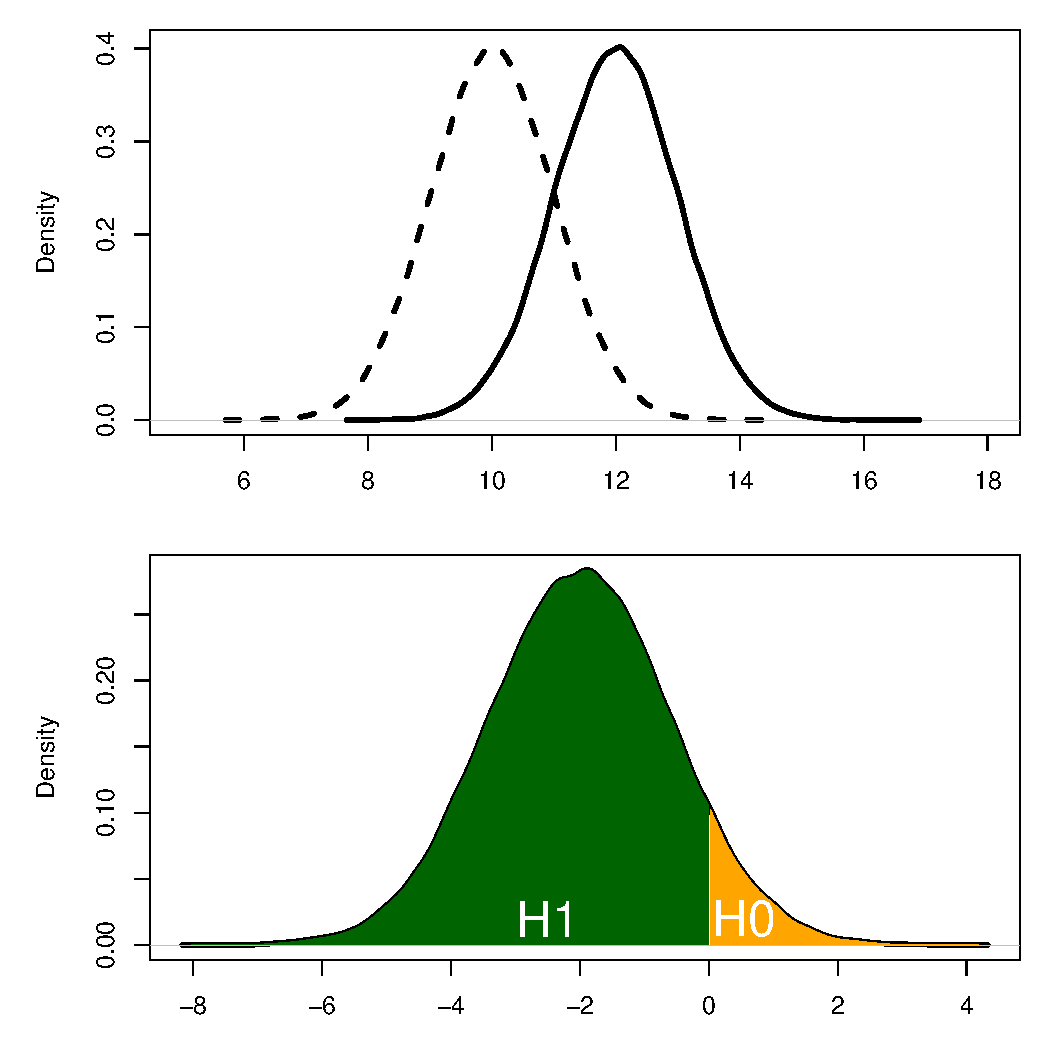
\includegraphics[width=.6\textwidth]{proba}}
\rput[b](3,7){$\mu_{ij}$}
\rput[b](7.5,7){$\mu_{i'j}$}
\rput[b](3,3){$\mu_{ij} - \mu_{i'j}$}
\end{pspicture}
\end{center}
\caption{Mean comparison between $\mu_{ij}$ (dash line) and $\mu_{i'j}$ (plain line).}
\label{proba}
\end{figure}

%% R code to get proba.pdf %%
%
%pdf("proba.pdf")
%
%par(mfrow=c(2,1),mar=c(3,5,1,1))
%
%a = rnorm(100000,10)
%d <- density(a)
%plot(d, type='l', xlab="", main="", xlim=c(5,18), lty=2, lwd=3)
%
%b = rnorm(100000,12)
%d <- density(b)
%lines(d,lty=1, lwd=3)
%
%diff = a - b
%
%d <- density(diff)
%plot(d, type='l', xlab="", main="", lty=1, lwd=3)
%
%toget = which(d$x>=0)
%H0x = d$x[toget]
%H0y = d$y[toget]
%
%toget = which(d$x<0)
%H1x = d$x[toget]
%H1y = d$y[toget]
%
%x <- H0x
%y <- H0y
%polygon( c(x,rev(x)), c(rep(0,length(x)),rev(y)), border=NA, col="orange" )
%
%x <- H1x
%y <- H1y
%polygon( c(x,rev(x)), c(rep(0,length(x)),rev(y)), border=NA, col="darkgreen" )
%
%text(-2.5,0.02,"H1", cex=2, col="white")
%text(0.55,0.02,"H0", cex=2, col="white")
%
%dev.off()





\paragraph{Computation}

In \pack, mean comparisons are done with \texttt{get.mean.comparisons}.
You can choose on which parameters to run the comparison (\texttt{parameter} argument) and the $\alpha$ type one error (\texttt{alpha} argument).
The soft Bonferonni correction is applied by default (\texttt{p.adj} argument).
More informations on this function by typing \texttt{?get.mean.comparisons}.

\begin{knitrout}
\definecolor{shadecolor}{rgb}{0.969, 0.969, 0.969}\color{fgcolor}\begin{kframe}
\begin{alltt}
\hlcom{# comp.mu = get.mean.comparisons(out1$MCMC, "mu")}
\hlcom{# Get at least X groups for env2-1:2011. It may take some time ...}
\hlcom{# Get at least X groups for  env2-1:2011 is done.}
\hlcom{# Get at least X groups for env2-13:2011. It may take some time ...}
\hlcom{# Get at least X groups for  env2-13:2011 is done.}
\hlcom{# Get at least X groups for env2-3:2012. It may take some time ...}
\hlcom{# Get at least X groups for  env2-3:2012 is done.}
\hlcom{# Get at least X groups for env2-9:2010. It may take some time ...}
\hlcom{# Get at least X groups for  env2-9:2010 is done.}

\hlkwd{load}\hlstd{(}\hlstr{"./data_PPBstats/comp.mu.RData"}\hlstd{)} \hlcom{# To save time}
\end{alltt}
\end{kframe}
\end{knitrout}

\paragraph{Plots}

\subparagraph{All entries in a given environment}

To see the output, use \texttt{get.ggplot}.
On each plot, the \texttt{alpha} (type one error) value and the alpha correction are displayed.
\texttt{alpha = Imp} means that no differences were possible to find.
For \texttt{ggplot.type = "interaction"} and \texttt{ggplot.type = "score"}, it is display under the form: \texttt{alpha | alpha correction}.

\begin{knitrout}
\definecolor{shadecolor}{rgb}{0.969, 0.969, 0.969}\color{fgcolor}\begin{kframe}
\begin{alltt}
\hlstd{p_barplot} \hlkwb{=} \hlkwd{get.ggplot}\hlstd{(comp.mu,} \hlkwc{ggplot.type} \hlstd{=} \hlstr{"barplot"}\hlstd{)}
\hlkwd{length}\hlstd{(p_barplot)}
\end{alltt}
\begin{verbatim}
## [1] 58
\end{verbatim}
\begin{alltt}
\hlkwd{names}\hlstd{(p_barplot)}
\end{alltt}
\begin{verbatim}
##  [1] "env1-1:2010"  "env1-1:2011"  "env1-1:2012"  "env1-2:2010" 
##  [5] "env1-2:2011"  "env1-2:2012"  "env1-3:2010"  "env1-3:2011" 
##  [9] "env1-3:2012"  "env1-4:2010"  "env1-4:2011"  "env1-4:2012" 
## [13] "env1-5:2011"  "env2-10:2010" "env2-10:2011" "env2-10:2012"
## [17] "env2-11:2011" "env2-11:2012" "env2-1:2010"  "env2-1:2011" 
## [21] "env2-1:2012"  "env2-12:2011" "env2-12:2012" "env2-13:2011"
## [25] "env2-13:2012" "env2-14:2011" "env2-14:2012" "env2-15:2011"
## [29] "env2-15:2012" "env2-2:2010"  "env2-2:2011"  "env2-2:2012" 
## [33] "env2-3:2010"  "env2-3:2011"  "env2-3:2012"  "env2-4:2010" 
## [37] "env2-4:2011"  "env2-4:2012"  "env2-5:2010"  "env2-5:2011" 
## [41] "env2-5:2012"  "env2-6:2010"  "env2-6:2011"  "env2-6:2012" 
## [45] "env2-7:2010"  "env2-7:2011"  "env2-7:2012"  "env2-8:2010" 
## [49] "env2-8:2011"  "env2-8:2012"  "env2-9:2010"  "env2-9:2011" 
## [53] "env2-9:2012"  "env3-1:2011"  "env3-1:2012"  "env3-2:2011" 
## [57] "env3-2:2012"  "env3-3:2011"
\end{verbatim}
\end{kframe}
\end{knitrout}

\begin{figure}[H]

\begin{knitrout}
\definecolor{shadecolor}{rgb}{0.969, 0.969, 0.969}\color{fgcolor}\begin{kframe}
\begin{alltt}
\hlcom{# For environment env-1-1:2010}
\hlkwd{grid.arrange}\hlstd{(p_barplot}\hlopt{$}\hlstr{"env1-1:2010"}\hlstd{[[}\hlnum{1}\hlstd{]], p_barplot}\hlopt{$}\hlstr{"env1-1:2010"}\hlstd{[[}\hlnum{2}\hlstd{]] ,} \hlkwc{ncol} \hlstd{=} \hlnum{2}\hlstd{,} \hlkwc{nrow} \hlstd{=} \hlnum{1}\hlstd{)}
\hlkwd{grid.arrange}\hlstd{(p_barplot}\hlopt{$}\hlstr{"env1-1:2010"}\hlstd{[[}\hlnum{2}\hlstd{]], p_barplot}\hlopt{$}\hlstr{"env1-1:2010"}\hlstd{[[}\hlnum{4}\hlstd{]],} \hlkwc{ncol} \hlstd{=} \hlnum{2}\hlstd{,} \hlkwc{nrow} \hlstd{=} \hlnum{1}\hlstd{)}
\end{alltt}
\end{kframe}

{\centering 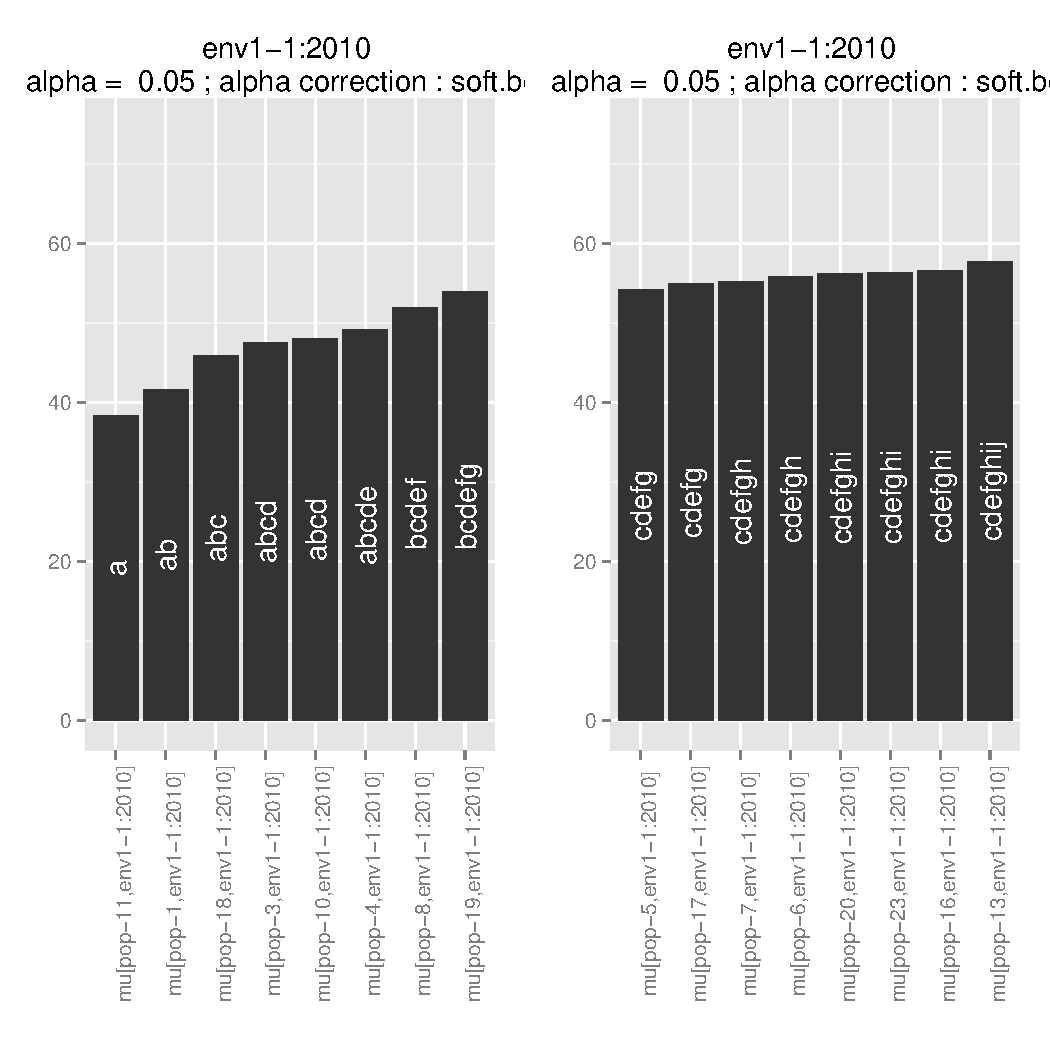
\includegraphics[width=.6\textwidth]{figures/PPBstats_unnamed-chunk-20-1} 
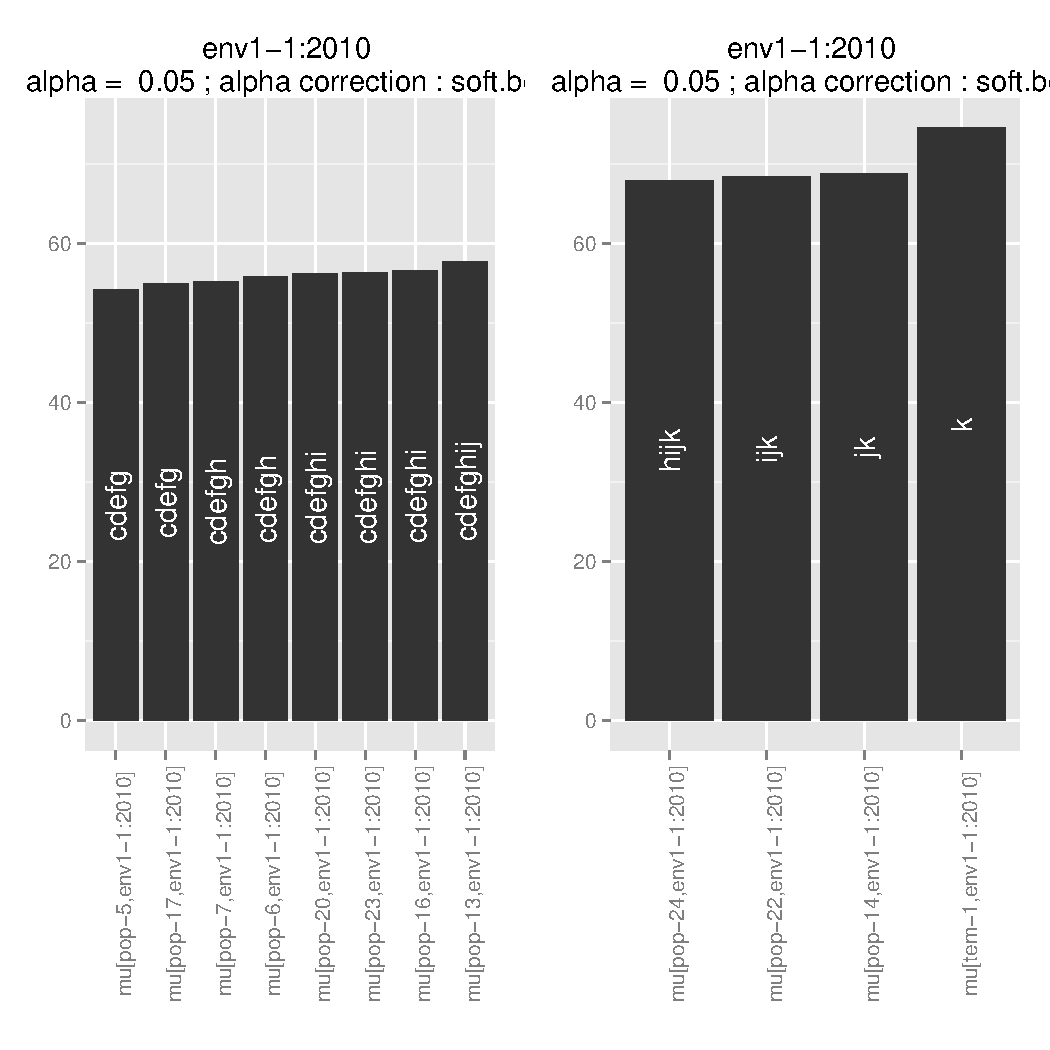
\includegraphics[width=.6\textwidth]{figures/PPBstats_unnamed-chunk-20-2} 

}



\end{knitrout}
\end{figure}

With \texttt{ggplot.type = "interaction"}, you can display the year effect as well as detect groups.
One group is represented by one dashed line.
Germplasms which share the same group are not different.
Germplasms which do not share the same groupe are different (section \ref{mean_comp}).

\begin{knitrout}
\definecolor{shadecolor}{rgb}{0.969, 0.969, 0.969}\color{fgcolor}\begin{kframe}
\begin{alltt}
\hlstd{p_interaction} \hlkwb{=} \hlkwd{get.ggplot}\hlstd{(comp.mu,} \hlkwc{ggplot.type} \hlstd{=} \hlstr{"interaction"}\hlstd{)}
\end{alltt}
\end{kframe}
\end{knitrout}

\begin{figure}[H]
\begin{knitrout}
\definecolor{shadecolor}{rgb}{0.969, 0.969, 0.969}\color{fgcolor}\begin{kframe}
\begin{alltt}
\hlcom{# For location env-1-1.}
\hlstd{p_interaction}\hlopt{$}\hlstr{"env1-1"}\hlstd{[[}\hlnum{1}\hlstd{]]}
\end{alltt}
\end{kframe}

{\centering 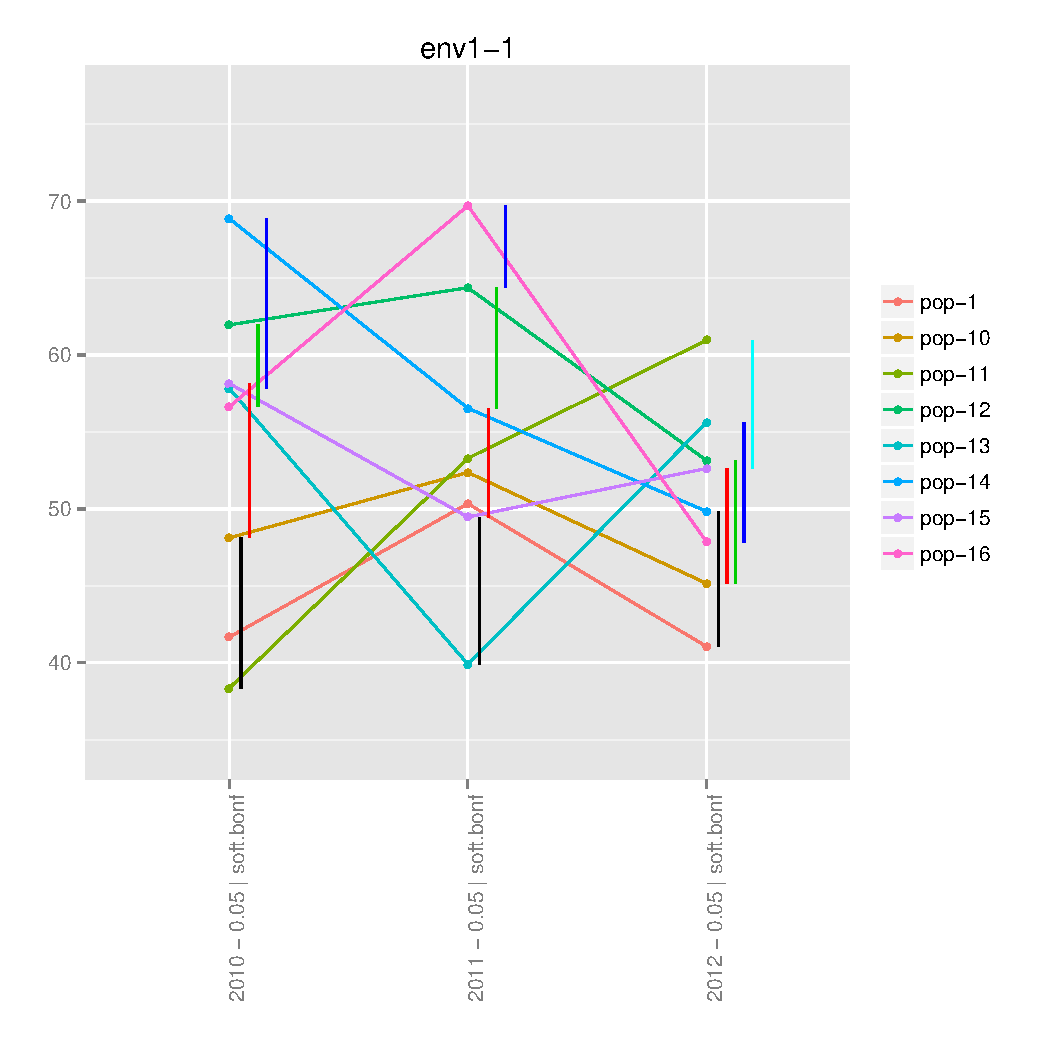
\includegraphics[width=.6\textwidth]{figures/PPBstats_unnamed-chunk-22-1} 

}



\end{knitrout}
\end{figure}

\begin{figure}[H]
\begin{knitrout}
\definecolor{shadecolor}{rgb}{0.969, 0.969, 0.969}\color{fgcolor}\begin{kframe}
\begin{alltt}
\hlstd{p_interaction}\hlopt{$}\hlstr{"env1-1"}\hlstd{[[}\hlnum{2}\hlstd{]]}
\end{alltt}
\end{kframe}

{\centering 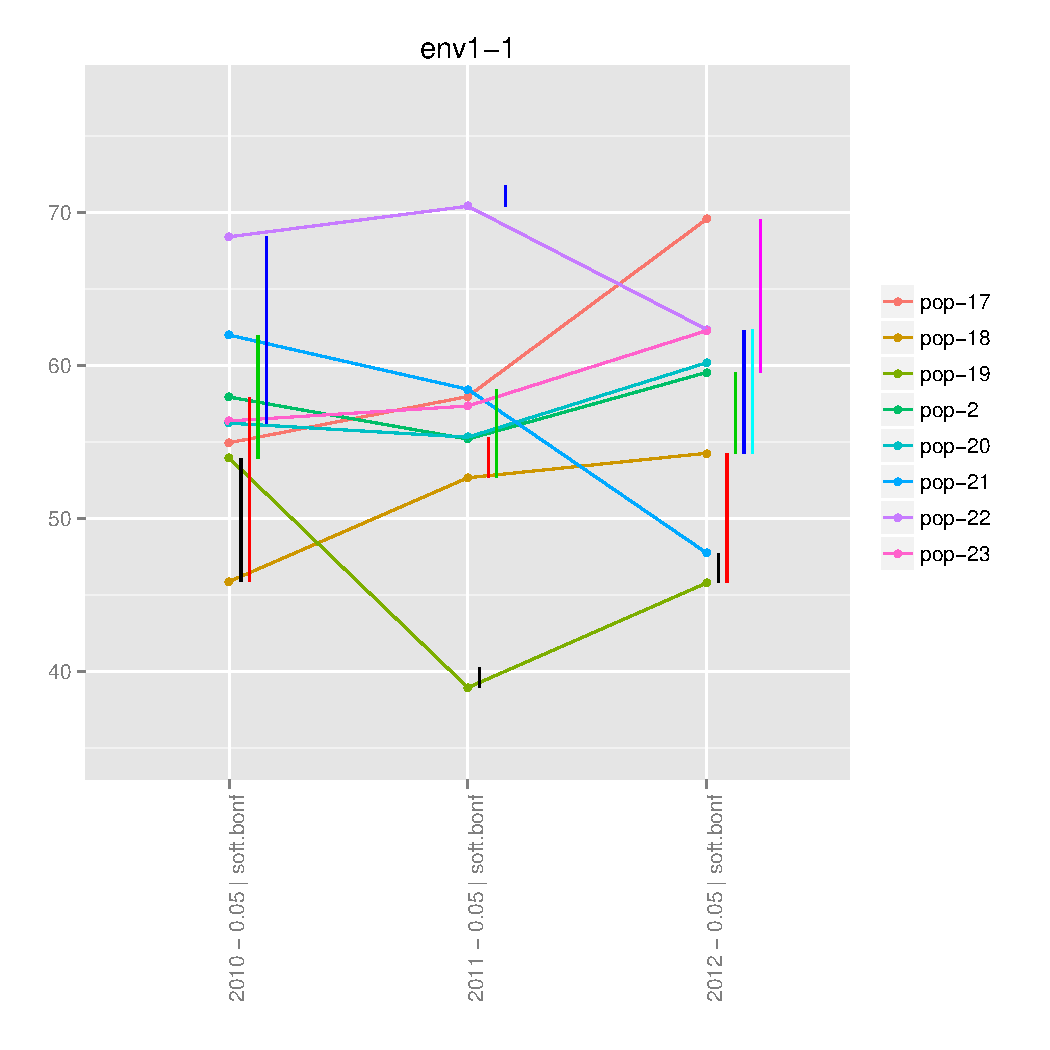
\includegraphics[width=.6\textwidth]{figures/PPBstats_unnamed-chunk-23-1} 

}



\end{knitrout}
\end{figure}

\begin{figure}[H]
\begin{knitrout}
\definecolor{shadecolor}{rgb}{0.969, 0.969, 0.969}\color{fgcolor}\begin{kframe}
\begin{alltt}
\hlstd{p_interaction}\hlopt{$}\hlstr{"env1-1"}\hlstd{[[}\hlnum{3}\hlstd{]]}
\end{alltt}
\end{kframe}

{\centering 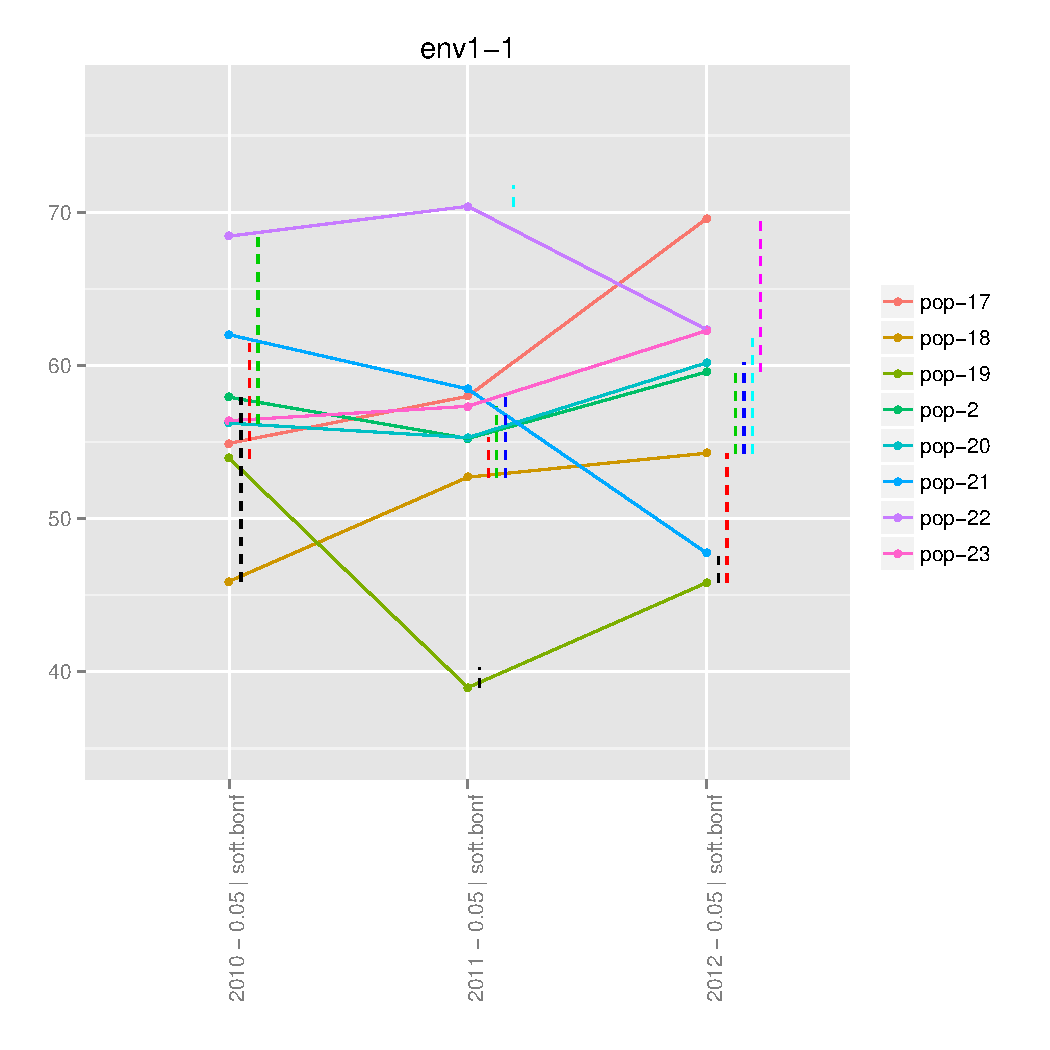
\includegraphics[width=.6\textwidth]{figures/PPBstats_unnamed-chunk-24-1} 

}



\end{knitrout}
\end{figure}
             
\begin{figure}[H]
\begin{knitrout}
\definecolor{shadecolor}{rgb}{0.969, 0.969, 0.969}\color{fgcolor}\begin{kframe}
\begin{alltt}
\hlstd{p_interaction}\hlopt{$}\hlstr{"env1-1"}\hlstd{[[}\hlnum{4}\hlstd{]]}
\end{alltt}
\end{kframe}

{\centering 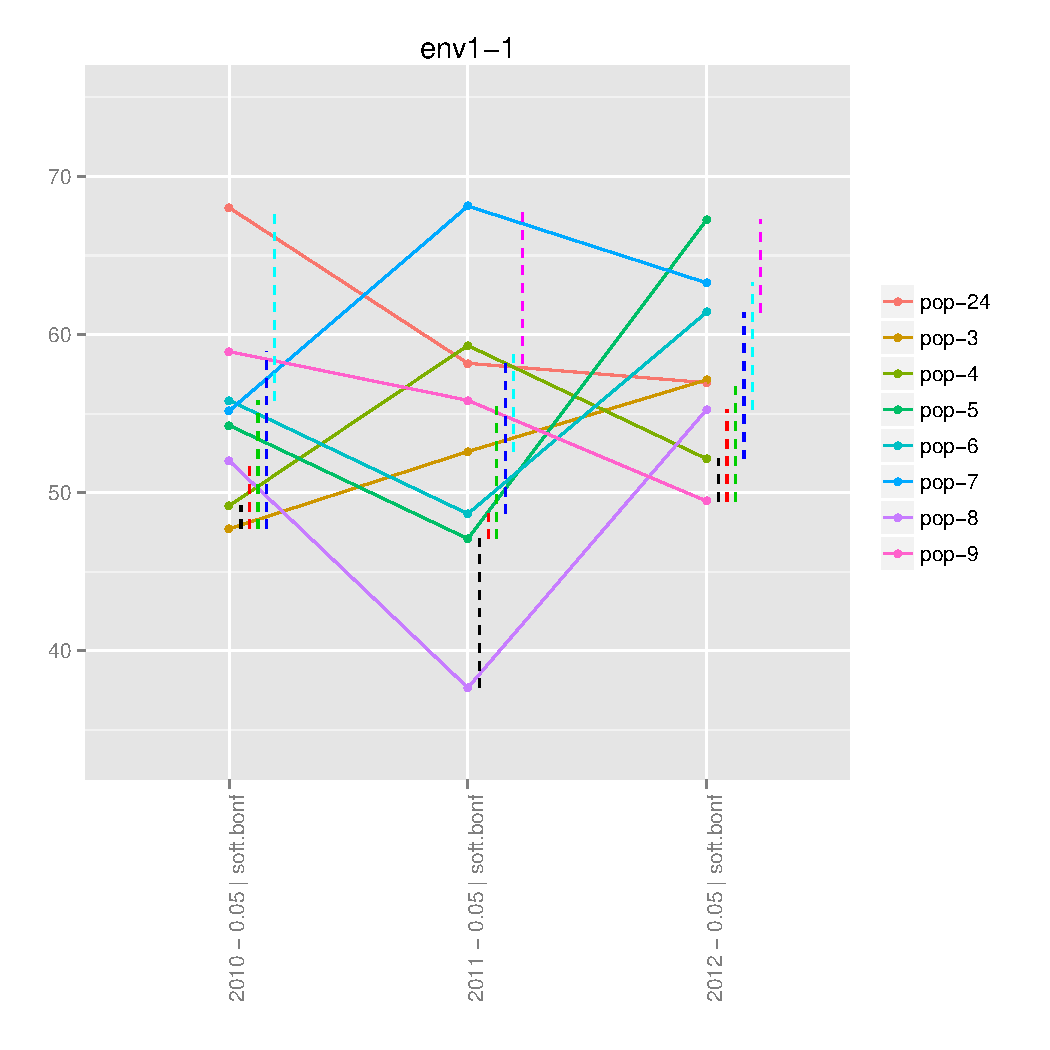
\includegraphics[width=.6\textwidth]{figures/PPBstats_unnamed-chunk-25-1} 

}



\end{knitrout}
\end{figure}

For the score, more entries are displayed.
An high score means that the entry was in a group with an high mean.
A low socre means that the entry was in a group with an low mean.
This plot is useful to look at year effects.

\begin{figure}[H]
\begin{knitrout}
\definecolor{shadecolor}{rgb}{0.969, 0.969, 0.969}\color{fgcolor}\begin{kframe}
\begin{alltt}
\hlstd{p_score} \hlkwb{=} \hlkwd{get.ggplot}\hlstd{(comp.mu,} \hlkwc{ggplot.type} \hlstd{=} \hlstr{"score"}\hlstd{,} \hlkwc{nb_parameters_per_plot} \hlstd{=} \hlnum{15}\hlstd{)}
\hlcom{# For location env-1-1}
\hlkwd{grid.arrange}\hlstd{(p_score}\hlopt{$}\hlstr{"env1-1"}\hlstd{[[}\hlnum{1}\hlstd{]], p_score}\hlopt{$}\hlstr{"env1-1"}\hlstd{[[}\hlnum{2}\hlstd{]] ,} \hlkwc{ncol} \hlstd{=} \hlnum{2}\hlstd{,} \hlkwc{nrow} \hlstd{=} \hlnum{1}\hlstd{)}
\end{alltt}
\end{kframe}

{\centering 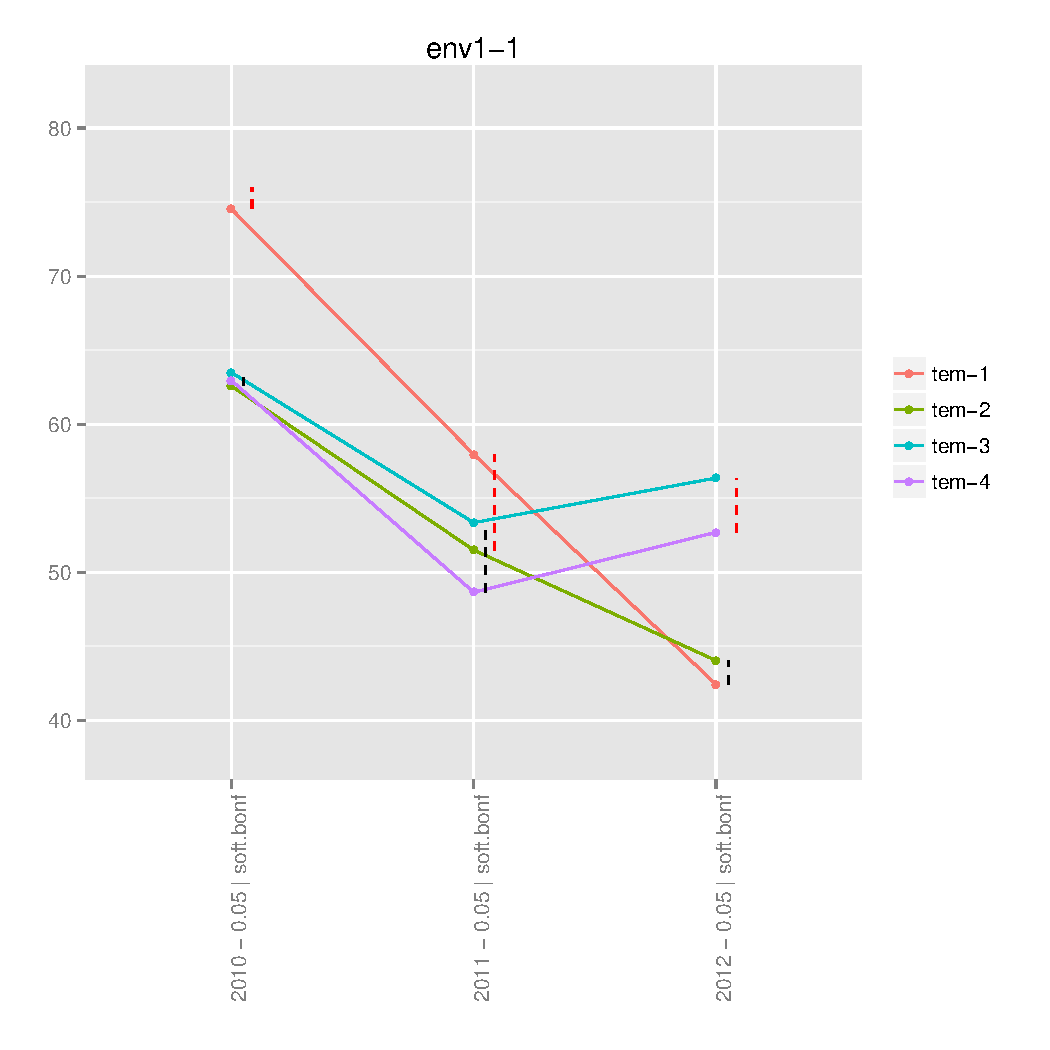
\includegraphics[width=.6\textwidth]{figures/PPBstats_unnamed-chunk-26-1} 

}



\end{knitrout}
\end{figure}

The same method is used for each $\beta_{jk}$.

\vspace{.5cm}

For environments with no controls or where at least one MCMC did not converge, it may be useful to get the plot as well.

\begin{figure}[H]
\begin{knitrout}
\definecolor{shadecolor}{rgb}{0.969, 0.969, 0.969}\color{fgcolor}\begin{kframe}
\begin{alltt}
\hlkwd{get.ggplot}\hlstd{(out.model1}\hlopt{$}\hlstd{data_env_with_no_controls,} \hlkwc{ggplot.type} \hlstd{=} \hlstr{"barplot"}\hlstd{)}
\end{alltt}
\begin{verbatim}
## $`env5:2010`
## $`env5:2010`$`1`
\end{verbatim}
\end{kframe}



{\centering 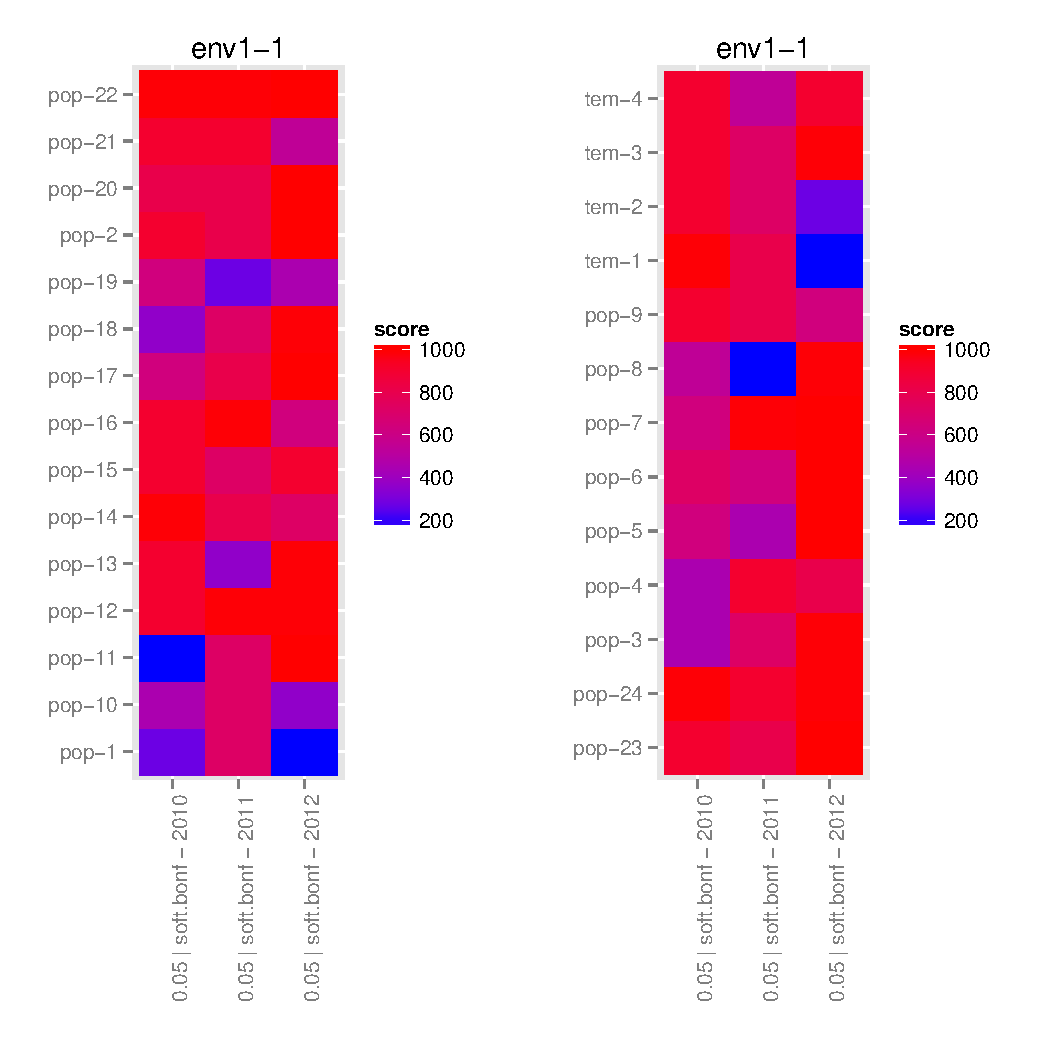
\includegraphics[width=.6\textwidth]{figures/PPBstats_unnamed-chunk-27-1} 

}



\end{knitrout}
\end{figure}

You can also do a plot with interaction. 
Here it is not useful as there is only one year.

\begin{figure}[H]
\begin{knitrout}
\definecolor{shadecolor}{rgb}{0.969, 0.969, 0.969}\color{fgcolor}\begin{kframe}
\begin{alltt}
\hlstd{g} \hlkwb{=} \hlkwd{get.ggplot}\hlstd{(out1_bis}\hlopt{$}\hlstd{model1.data_env_whose_param_did_not_converge,} \hlkwc{ggplot.type} \hlstd{=} \hlstr{"barplot"}\hlstd{)}

\hlkwd{names}\hlstd{(g)}
\end{alltt}
\begin{verbatim}
## [1] "env1-1:2012"  "env1-2:2011"  "env2-12:2012" "env2-6:2010"
\end{verbatim}
\begin{alltt}
\hlstd{g}\hlopt{$}\hlstd{`env1-1:2012`}\hlopt{$}\hlstd{`1`}
\end{alltt}
\end{kframe}

{\centering 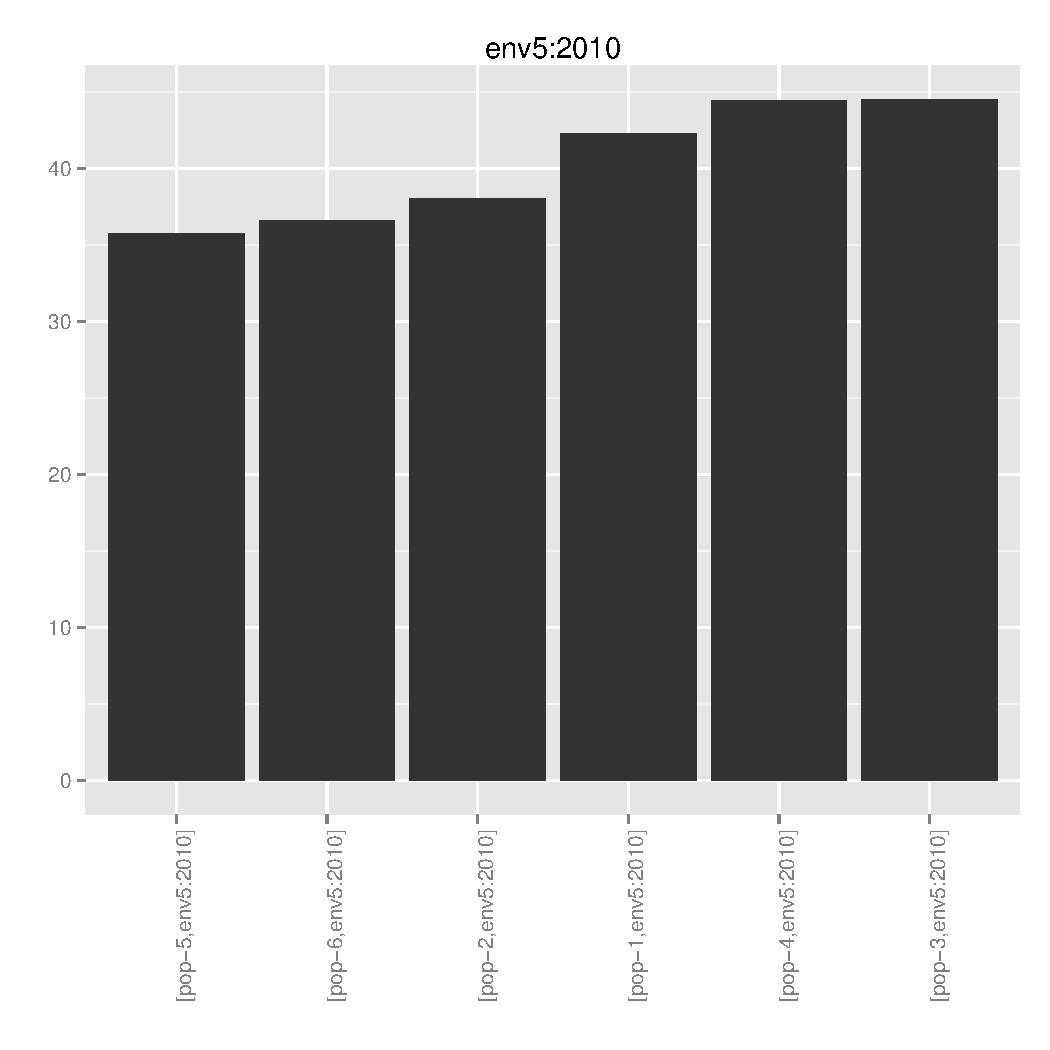
\includegraphics[width=.6\textwidth]{figures/PPBstats_unnamed-chunk-28-1} 

}



\end{knitrout}
\end{figure}


\subparagraph{Pairs of entries in a given environment}
It is possible to get comparison of paris of entries in a given location.
This is useful if you want to compare two versions within a group.
For exemple:

\begin{knitrout}
\definecolor{shadecolor}{rgb}{0.969, 0.969, 0.969}\color{fgcolor}\begin{kframe}
\begin{alltt}
\hlkwd{data}\hlstd{(data_version)}
\hlkwd{head}\hlstd{(data_version)}
\end{alltt}
\begin{verbatim}
##   year location germplasm group version
## 1 2010   env1-1     tem-1     1      v1
## 2 2010   env1-1     tem-2     1      v2
## 3 2010   env1-1     pop-1     2      v1
## 4 2010   env1-1     pop-2     2      v2
## 5 2010   env1-2     tem-1     3      v1
## 6 2010   env1-2     tem-2     3      v2
\end{verbatim}
\end{kframe}
\end{knitrout}

Here, in location \texttt{env1-1}, \texttt{tem-1} and \texttt{tem-2} are two version belonging to the same groupe.

Lets' make the plots:
\begin{knitrout}
\definecolor{shadecolor}{rgb}{0.969, 0.969, 0.969}\color{fgcolor}\begin{kframe}
\begin{alltt}
\hlstd{g} \hlkwb{=} \hlkwd{get.ggplot}\hlstd{(}\hlkwc{data} \hlstd{= comp.mu,} \hlkwc{data_version} \hlstd{= data_version,} \hlkwc{ggplot.type} \hlstd{=} \hlstr{"barplot"}\hlstd{)}
\end{alltt}


{\ttfamily\noindent\color{warningcolor}{\#\# Warning in get.ggplot(data = comp.mu, data\_version = data\_version, ggplot.type = "{}barplot"{}): The following environments in data\_version are not taken: env5:2010.}}\begin{alltt}
\hlstd{g}\hlopt{$}\hlstd{`env1-1:2010`}\hlopt{$}\hlstd{`1`}
\end{alltt}
\end{kframe}

{\centering 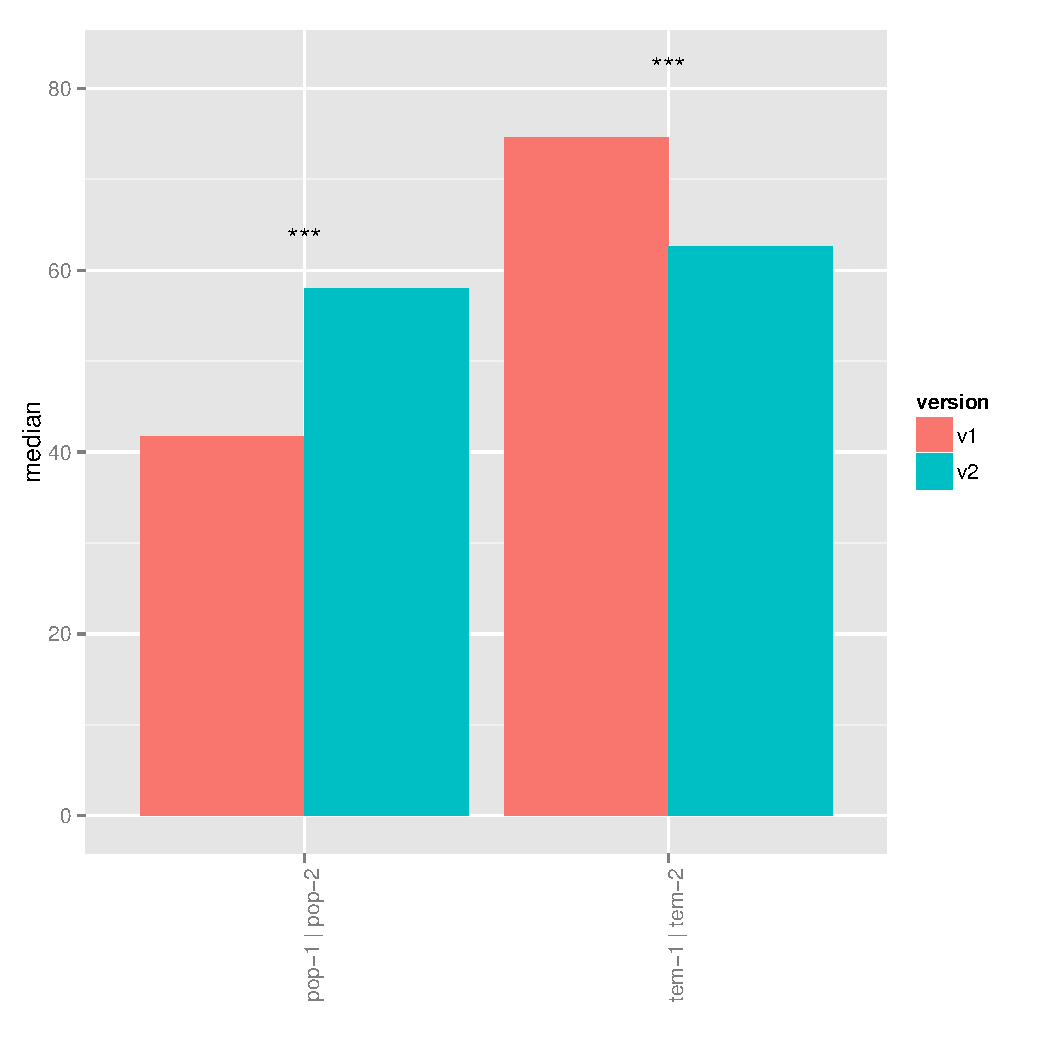
\includegraphics[width=.6\textwidth]{figures/PPBstats_unnamed-chunk-30-1} 

}



\end{knitrout}

The stars corresponds to the pvalue:

\begin{center}
\begin{tabular}{cc}
\hline
pvalue & stars \\
\hline
$< 0.001$ & *** \\
$[0.001 , 0.05]$ & ** \\
$[0.05 , 0.01]$ & * \\
$> 0.01$ & . \\
\hline
\end{tabular}
\end{center}

The pvalue is computed as describe in section \ref{mean_comp} if the parameters have been estimated with the model.

It is also possible to make this kind of plots for data that did not converge or without environments.
In this case, it is a \texttt{t.test} which is perform.

\begin{knitrout}
\definecolor{shadecolor}{rgb}{0.969, 0.969, 0.969}\color{fgcolor}\begin{kframe}
\begin{alltt}
\hlstd{g} \hlkwb{=} \hlkwd{get.ggplot}\hlstd{(out1_bis}\hlopt{$}\hlstd{model1.data_env_whose_param_did_not_converge,} \hlkwc{data_version} \hlstd{= data_version,} \hlkwc{ggplot.type} \hlstd{=} \hlstr{"barplot"}\hlstd{)}
\end{alltt}


{\ttfamily\noindent\color{warningcolor}{\#\# Warning in get.ggplot(out1\_bis\$model1.data\_env\_whose\_param\_did\_not\_converge, : The following environments in data\_version are not taken: env1-1:2010, env1-2:2010, env5:2010.}}

{\ttfamily\noindent\color{warningcolor}{\#\# Warning in FUN(X[[i]], ...): No t.test are done as there are not enough observations.}}\begin{alltt}
\hlstd{g} \hlkwb{=} \hlkwd{get.ggplot}\hlstd{(out.model1}\hlopt{$}\hlstd{data_env_with_no_controls,} \hlkwc{data_version} \hlstd{= data_version,} \hlkwc{ggplot.type} \hlstd{=} \hlstr{"barplot"}\hlstd{)}
\end{alltt}


{\ttfamily\noindent\color{warningcolor}{\#\# Warning in get.ggplot(out.model1\$data\_env\_with\_no\_controls, data\_version = data\_version, : The following environments in data\_version are not taken: env1-1:2010, env1-2:2010, env1-1:2012.}}

{\ttfamily\noindent\color{warningcolor}{\#\# Warning in FUN(X[[i]], ...): No t.test are done as there are not enough observations.}}\end{kframe}
\end{knitrout}


\section{At the network level : model~\ref{model2} to analyse $G \times E$ interaction in the network of farms }
\label{section_model2}

\subsection{The model}
The phenotypic value $Y_{ij}$ for a given variable $Y$, germplasm $i$ and environment $j$, was modeled as :

\begin{displaymath}
Y_{ij} = \alpha_{i} + \theta_{j} + \eta_{i}\theta_{j} + \varepsilon_{ij} ; \quad \varepsilon_{ij} \sim \mathcal{N} (0,\sigma^2_{e}),
\label{modele_gxe}
\end{displaymath}

for $i = 1,\ldots, I$ and $j = 1,\ldots, J$, where 
$I$ was the number of germplasms, 
$J$ was the number of environments,
$\alpha_{i}$ was the main effect of germplasm $i$,
$\theta_{j}$ was the main effect of environnment $j$,
$\varepsilon_{ij}$ was the residual and 
$\mathcal{N} (0,\sigma^2_{e})$ was the normal distribution with mean 0 and variance $\sigma^2_{e}$.
The interaction between germplasm $i$ and environment $j$ was divided into a multiplicative term $\eta_{i}\theta_{j}$ and a remaining term that contributed to the residual $\varepsilon_{ij}$.

This model was written as :

\begin{equation}
Y_{ij}  = \alpha_{i} + \beta_{i} \theta_{j} + \varepsilon_{ij}; \quad \varepsilon_{ij} \sim \mathcal{N} (0,\sigma_{\varepsilon}),
	\label{model2}
\end{equation}

Where $\beta_{i} = (1 + \eta_{i})$ was the sensitivity of germplasm $i$ to environments.
This model is known as the Finlay Wilkinson model or as joint regression \citep{finlay_analysis_1963}.
Germplasm sensitivities quantified the stability of germplasm performances over environments.
The average sensitivity was equal to 1 so that a gemplasm with $\beta_{i} > 1$ ($\beta_{i} < 1$) was more (less) sensitive to environments than a germplasm with the average sensitivity \citep{nabugoomu_analysis_1999}.

Given the high disequilibrium of the data and the large amount of data, we decided to implement this model with a hierarchical Bayesian approach.
In the following, this Hierarchical Finlay Wilkinson model was denoted by HFW.

We used hierarchical priors for $\alpha_i$, $\beta_i$ and $\theta_j$ and a vague prior for $\sigma_{\varepsilon}$.

\begin{displaymath}
\alpha_{i} \sim \mathcal{N} (\mu,\sigma^2_{\alpha}), \quad 
\beta_{i} \sim \mathcal{N} (1,\sigma^2_{\beta}), \quad 
\theta_{j} \sim \mathcal{N} (0,\sigma^2_{\theta}), \quad 
\sigma^{-2}_{\varepsilon} \sim \mathcal{G}amma (10^{-6},10^{-6}),
\end{displaymath}

where $\mu$, $\sigma^2_{\alpha}$, $\sigma^2_{\beta}$ and $\sigma^2_{\theta}$ were unknown parameters.
The mean of $\beta_i$ was set to 1 \citep{nabugoomu_analysis_1999}.


Then, we placed weakly-informative priors on the hyperparmeters  $\mu$, $\sigma^2_{\alpha}$, $\sigma^2_{\beta}$ and $\sigma^2_{\theta}$:

\begin{displaymath}
\mu \sim \mathcal{N} (\nu,\nu^2), \quad 
\sigma_{\alpha} \sim \mathcal{U}niforme (0,\nu), \quad 
\sigma_{\beta} \sim \mathcal{U}niforme (0,1), \quad 
\sigma_{\theta} \sim \mathcal{U}niforme (0,\nu),
\end{displaymath}

where $\nu$ was the arithmetic mean of the data : $\nu = \sum_{ij} {Y_{ij}/n}$ where $n$ was the number of observations.
Uniform priors were used for $\sigma^2_{\alpha}$, $\sigma^2_{\beta}$ and $\sigma^2_{\theta}$ to reduce the influence of these priors on posterior results \citep{gelman__2006}.
The support of these priors took account of the prior knowledge that $\sigma^2_{\alpha}$, $\sigma^2_{\beta}$ and $\sigma^2_{\theta}$ were expected to be respectively smaller than $\nu$, 1, $\nu$. \\

Initial values for each chain were taken randomly except for $\mu$, $\sigma_{\alpha}$ and $\sigma_{\theta}$ whose initial values were equal to their posterior median from additive model (i.e. model \ref{model2} with $\forall i, \beta_{i}=1$). \\


The main parameter of interest were 
germplasm main effects ($\alpha_{i}, i = 1,\ldots, I$), 
environment main effects ($\theta_{j}, j = 1,\ldots, J$) and 
germplasm sensitivities ($\beta_{i}, i = 1,\ldots, I$).
For $\alpha_i$, the average posterior response of each germplasm over the environments of the network was considered:

\begin{displaymath}
\gamma_i = \alpha_i + \beta_{i} \bar{\theta},
\end{displaymath}
where
$\bar{\theta} = \sum_{}^{J} \theta_j/J$.

To simplify, the $\alpha_i$ notation is kept instead of $\gamma_i$ (i.e. $\alpha_i = \gamma_i$).
But keep in mind it has been corrected.


\subsection{With \pack}

For model~\ref{model2}, you can follow these steps (Figure \ref{function_relations}):

\begin{enumerate}
\item Run the model with \texttt{FWH}
\item Analyse model outputs with graphs to kow if you can continue the analysis with \texttt{analyse.outputs}
\item Perform cross validation studies with \texttt{cross.validation.FWH} in order to assess the quality of the model
\item Get mean comparisons for each factor with \texttt{get.mean.comparisons} and \texttt{get.ggplot}
\item Get groups of parameters for $\alpha$, $\beta$ and $\theta$ with \texttt{get.parameters.groups} and \texttt{get.ggplot}
\item Predict the past with \texttt{predict.the.past} and \texttt{get.ggplot}
\end{enumerate}

Let's get the data.
The values for $\alpha_i$, $\beta_i$, $\theta_j$ are the real value taken to create the dataset for y1.
This dataset is representative of data you can get in a PPB programme.

\begin{knitrout}
\definecolor{shadecolor}{rgb}{0.969, 0.969, 0.969}\color{fgcolor}\begin{kframe}
\begin{alltt}
\hlkwd{data}\hlstd{(PPBdata2)}
\hlkwd{head}\hlstd{(PPBdata2)}
\end{alltt}
\begin{verbatim}
##   germplasm location   year        y1 alpha_i-1 beta_i-1  theta_j-1
## 1     geno1   loc-35 year-1  7.926204  10.25349 2.170004 -0.7776704
## 2     geno1   loc-48 year-1  9.772076  10.25349 2.170004 -0.7531355
## 3     geno1   loc-20 year-5  9.199745  10.25349 2.170004  0.1163468
## 4     geno1   loc-33 year-5 10.131745  10.25349 2.170004  0.2755013
## 5     geno1   loc-44 year-3 14.329280  10.25349 2.170004  1.8495949
## 6     geno1   loc-34 year-1  8.709140  10.25349 2.170004 -0.5750281
##         y2       y3 block X Y
## 1 18.28223 31.57931     1 1 1
## 2 18.41129 31.44957     1 2 2
## 3 18.94209 33.19169     1 3 3
## 4 24.86338 29.34573     1 4 4
## 5 16.09421 32.36811     1 5 5
## 6 17.93222 37.85269     1 6 6
\end{verbatim}
\end{kframe}
\end{knitrout}


\subsubsection{Run the model}

To run model \ref{model2} on the dataset, used the function \texttt{FWH} (which stands for Finlay Wilkinson Hierarchical).
You can run it on one variable.
Here it is on thousand kernel weight (tkw)

By default, \texttt{FWH} returns posteriors for 
$\alpha_i$ (\texttt{return.alpha = TRUE}),
$\sigma_{\alpha}$ (\texttt{return.sigma\_alpha = TRUE}),
$\beta_i$ (\texttt{return.beta = TRUE}),
$\sigma_{\beta}$ (\texttt{return.sigma\_beta = TRUE}),
$\theta_j$ (\texttt{return.theta = TRUE}),
$\sigma_{\theta}$ (\texttt{return.sigma\_theta = TRUE}) and
$\sigma_{\epsilon}$ (\texttt{return.sigma\_epsilon = TRUE}).
You can also get $\epsilon_{ij}$ with \texttt{return.epsilon = TRUE}.

By default, DIC is not display, you may want this value to compare to other model (\texttt{DIC = TRUE}).
DIC criterion is a generalization of the AIC criterion that can be used for hierarchical models \citep{spiegelhalter_bayesian_2002}.
The smaller the DIC value, the better the model \citep{plummer_penalized_2008}.

\begin{knitrout}
\definecolor{shadecolor}{rgb}{0.969, 0.969, 0.969}\color{fgcolor}\begin{kframe}
\begin{alltt}
\hlcom{# out.model2 = FWH(data = PPBdata2, variable = "y1", return.epsilon = TRUE)}
\hlcom{#Run additive model ...}
\hlcom{#Compiling model graph}
\hlcom{#   Resolving undeclared variables}
\hlcom{#   Allocating nodes}
\hlcom{#   Graph Size: 9759}
\hlcom{#}
\hlcom{#Initializing model}
\hlcom{#}
\hlcom{#  |++++++++++++++++++++++++++++++++++++++++++++++++++| 100%}
\hlcom{#  |**************************************************| 100%}
\hlcom{#  |**************************************************| 100%}
\hlcom{#Run FWH model ...}
\hlcom{#Compiling model graph}
\hlcom{#   Resolving undeclared variables}
\hlcom{#   Allocating nodes}
\hlcom{#   Graph Size: 14677}
\hlcom{#}
\hlcom{#Initializing model}
\hlcom{#}
\hlcom{#  |++++++++++++++++++++++++++++++++++++++++++++++++++| 100%}
\hlcom{#  |**************************************************| 100%}
\hlcom{#  |**************************************************| 100%}
\hlcom{#  |**************************************************| 100%}

\hlkwd{load}\hlstd{(}\hlstr{"./data_PPBstats/out.model2.RData"}\hlstd{)} \hlcom{# To save time}
\end{alltt}
\end{kframe}
\end{knitrout}

It may be useful to see which germplasm were not use in the analysis because they were in only one environment.

\begin{knitrout}
\definecolor{shadecolor}{rgb}{0.969, 0.969, 0.969}\color{fgcolor}\begin{kframe}
\begin{alltt}
\hlstd{out.model2}\hlopt{$}\hlstd{germplasm.not.used}
\end{alltt}
\begin{verbatim}
## NULL
\end{verbatim}
\end{kframe}
\end{knitrout}

\subsubsection{Analysis of model outputs}

Once the model is run, it is necessary to check if the outputs can be taken with confidence. 
This step is needed before going ahead in the analysis (in fact, the MCMC object used in the next functions must come from \texttt{analyse.outputs}!).


\begin{knitrout}
\definecolor{shadecolor}{rgb}{0.969, 0.969, 0.969}\color{fgcolor}\begin{kframe}
\begin{alltt}
\hlcom{# out2 = analyse.outputs(out.model2)}
\hlcom{# The experimental design plot is done.}
\hlcom{# The Gelman-Rubin test is running for each parameter ...}
\hlcom{# The two MCMC for each parameter converge thanks to the Gelman-Rubin test.}
\hlcom{# The alpha_i posterior distributions are done.}
\hlcom{# The beta_i posterior distributions are done.}
\hlcom{# The theta_j posterior distributions are done.}
\hlcom{# The standardised residuals distributions are done.}

\hlkwd{load}\hlstd{(}\hlstr{"./data_PPBstats/out2.RData"}\hlstd{)} \hlcom{# To save time}
\end{alltt}
\end{kframe}
\end{knitrout}

\texttt{out2} is a list containing :

\begin{itemize}

\item "experimental\_design" : a plot representing the presence/abscence matrix of G $\times$ E combinaisons. 
Note that it displays only germplasms that are on at least two environments.

\begin{figure}[H]
\begin{knitrout}
\definecolor{shadecolor}{rgb}{0.969, 0.969, 0.969}\color{fgcolor}\begin{kframe}
\begin{alltt}
\hlstd{out2}\hlopt{$}\hlstd{data.experimental_design}\hlopt{$}\hlstd{plot}
\end{alltt}
\end{kframe}

{\centering 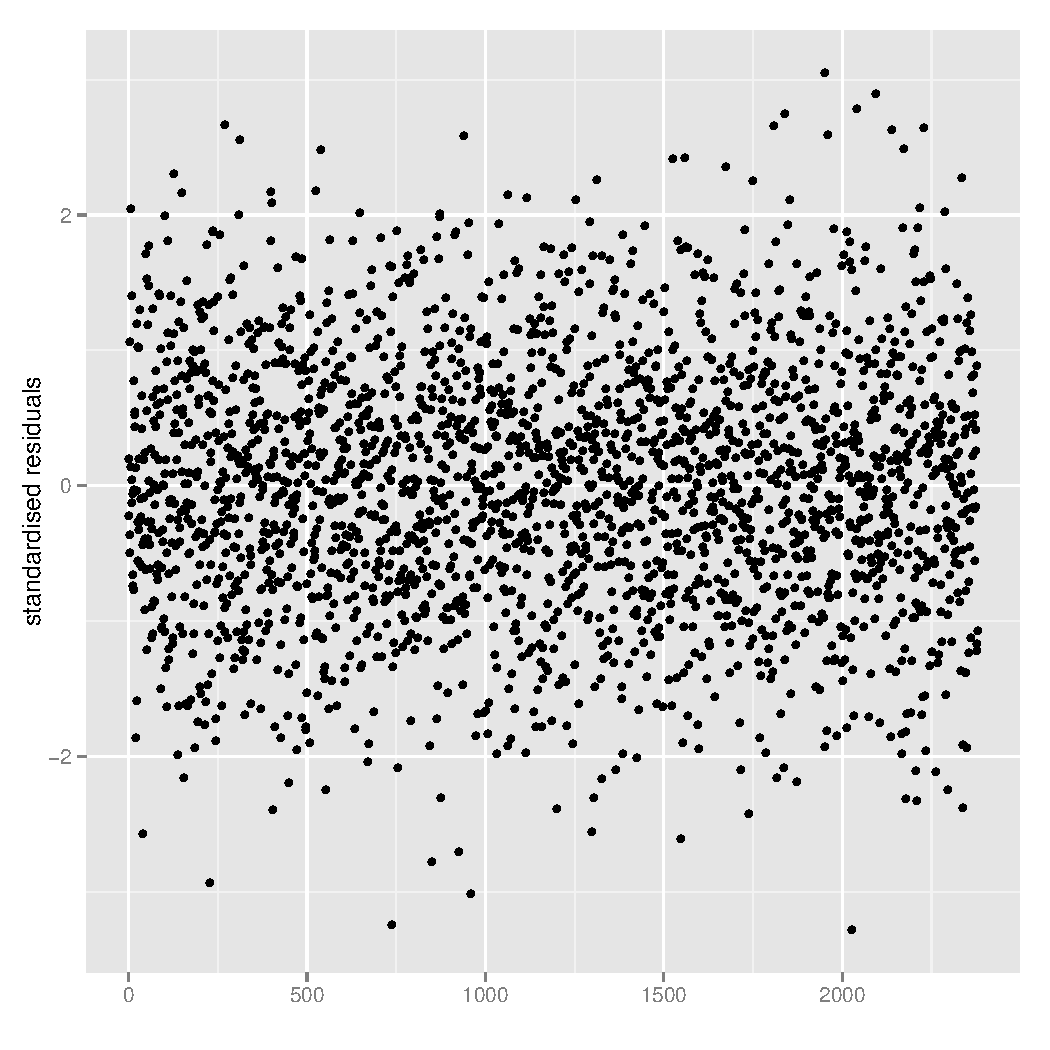
\includegraphics[width=.6\textwidth]{figures/PPBstats_unnamed-chunk-36-1} 

}



\end{knitrout}
\end{figure}

\item "convergence" : a list with the plots of trace and density to check the convergence of the two MCMC only for chains that are not converging thanks to the Gelman-Rubin test \citep{gelman_inference_1992}. If all the chains converge, it is NULL

\begin{figure}[H]
\begin{knitrout}
\definecolor{shadecolor}{rgb}{0.969, 0.969, 0.969}\color{fgcolor}\begin{kframe}
\begin{alltt}
\hlstd{out2}\hlopt{$}\hlstd{convergence}
\end{alltt}
\begin{verbatim}
## NULL
\end{verbatim}
\end{kframe}
\end{knitrout}
\end{figure}

\item "parameter\_posteriors": a list with caterpillar plot for each $\alpha_i$, $\beta_i$ and $\theta_j$.

Below an example for $\alpha_i$.

\begin{figure}[H]
\begin{knitrout}
\definecolor{shadecolor}{rgb}{0.969, 0.969, 0.969}\color{fgcolor}\begin{kframe}
\begin{alltt}
\hlstd{p} \hlkwb{=} \hlstd{out2}\hlopt{$}\hlstd{posteriors}\hlopt{$}\hlstd{parameter_posteriors}\hlopt{$}\hlstd{alpha_posteriors}
\hlkwd{grid.arrange}\hlstd{(p[[}\hlnum{1}\hlstd{]], p[[}\hlnum{2}\hlstd{]],}\hlkwc{ncol} \hlstd{=} \hlnum{2}\hlstd{,} \hlkwc{nrow} \hlstd{=} \hlnum{1}\hlstd{)}
\hlkwd{grid.arrange}\hlstd{(p[[}\hlnum{3}\hlstd{]], p[[}\hlnum{4}\hlstd{]],}\hlkwc{ncol} \hlstd{=} \hlnum{2}\hlstd{,} \hlkwc{nrow} \hlstd{=} \hlnum{1}\hlstd{)}
\end{alltt}
\end{kframe}

{\centering 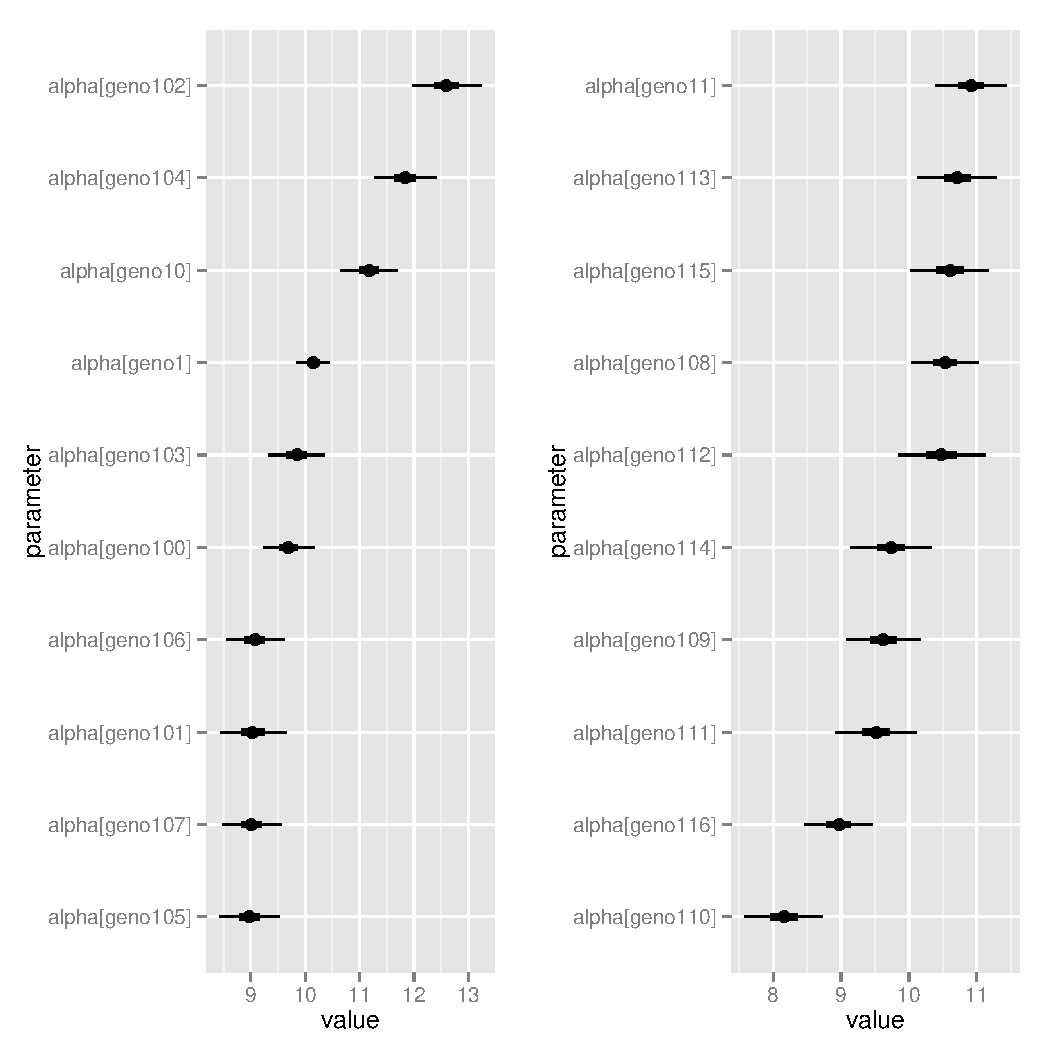
\includegraphics[width=.6\textwidth]{figures/PPBstats_unnamed-chunk-38-1} 
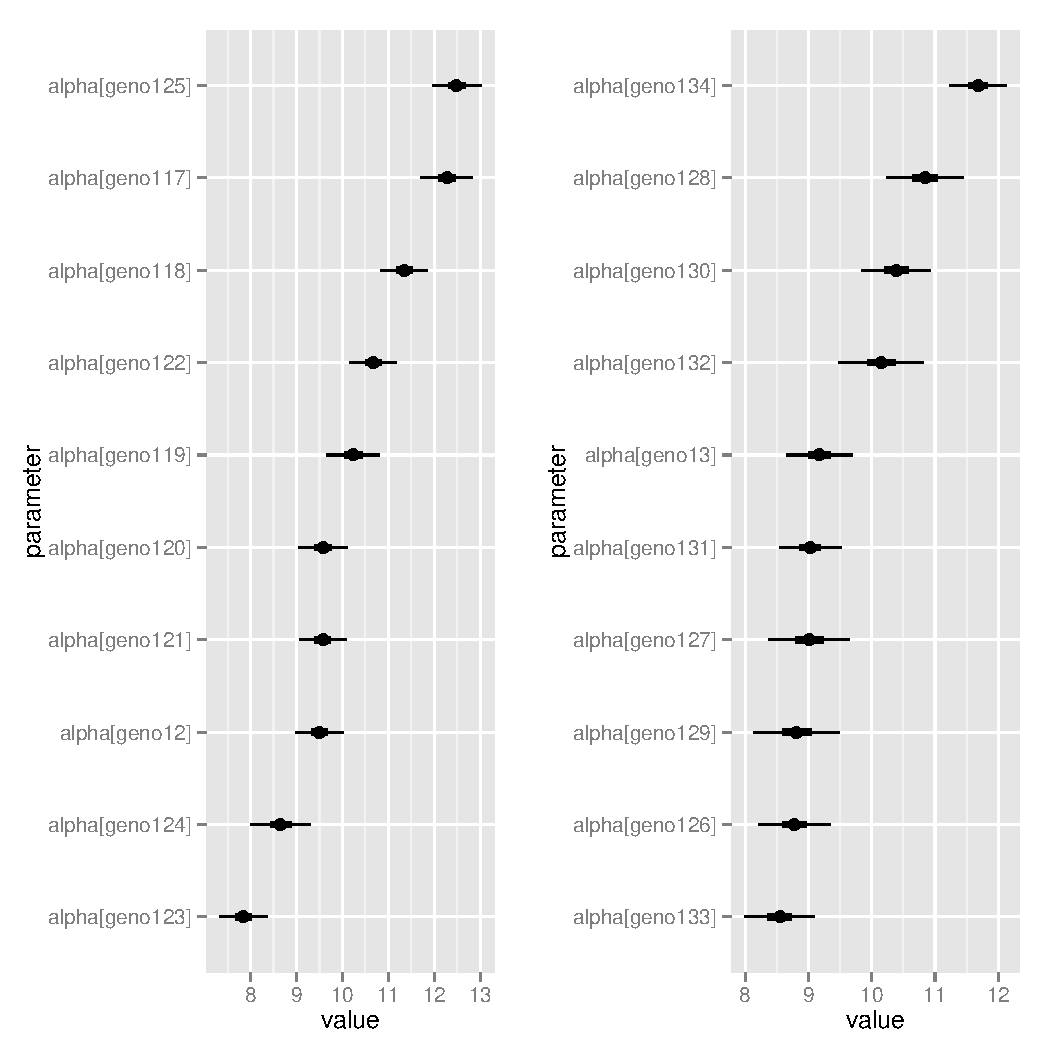
\includegraphics[width=.6\textwidth]{figures/PPBstats_unnamed-chunk-38-2} 

}



\end{knitrout}
\end{figure}


\item "standardized\_residuals" : a plot to check the normality of the residuals. If the model went well it should be between -2 and 2.

\begin{figure}[H]
\begin{knitrout}
\definecolor{shadecolor}{rgb}{0.969, 0.969, 0.969}\color{fgcolor}\begin{kframe}
\begin{alltt}
\hlstd{out2}\hlopt{$}\hlstd{posteriors}\hlopt{$}\hlstd{standardized_residuals}
\end{alltt}
\end{kframe}

{\centering 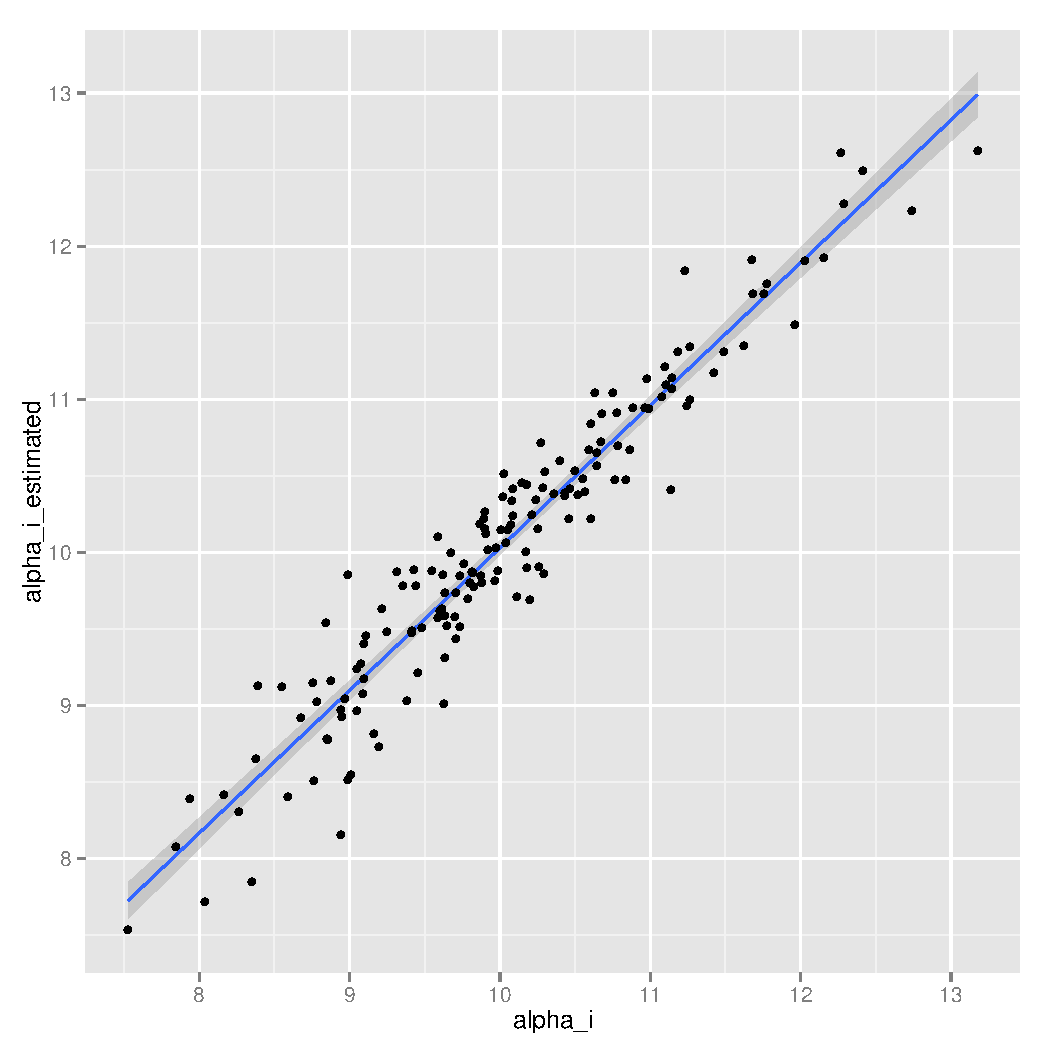
\includegraphics[width=.6\textwidth]{figures/PPBstats_unnamed-chunk-39-1} 

}



\end{knitrout}
\end{figure}

\item "MCMC": a data fame resulting from the concatenation of the two MCMC for each parameter. This object can be used for further analysis. There are as many columns than parameters and as many rows than iterations/thin (the thin value is 10 by default in the models).

\begin{knitrout}
\definecolor{shadecolor}{rgb}{0.969, 0.969, 0.969}\color{fgcolor}\begin{kframe}
\begin{alltt}
\hlkwd{dim}\hlstd{(out2}\hlopt{$}\hlstd{MCMC)}
\end{alltt}
\begin{verbatim}
## [1] 20000   385
\end{verbatim}
\end{kframe}
\end{knitrout}

\end{itemize}

Just for fun, you compare the posterior medians and the arithmetic means for the $\alpha_i$'s.

\begin{knitrout}
\definecolor{shadecolor}{rgb}{0.969, 0.969, 0.969}\color{fgcolor}\begin{kframe}
\begin{alltt}
\hlstd{MCMC} \hlkwb{=} \hlstd{out2}\hlopt{$}\hlstd{MCMC}
\hlstd{effects} \hlkwb{=} \hlkwd{apply}\hlstd{(MCMC,} \hlnum{2}\hlstd{, median)}
\hlstd{alpha_i_estimated} \hlkwb{=} \hlstd{effects[}\hlkwd{grep}\hlstd{(}\hlstr{"alpha\textbackslash{}\textbackslash{}["}\hlstd{,}\hlkwd{names}\hlstd{(effects))]}
\hlkwd{names}\hlstd{(alpha_i_estimated)} \hlkwb{=} \hlkwd{sapply}\hlstd{(}\hlkwd{names}\hlstd{(alpha_i_estimated),} \hlkwa{function}\hlstd{(}\hlkwc{x}\hlstd{)\{}
\hlkwd{sub}\hlstd{(}\hlstr{"\textbackslash{}\textbackslash{}]"}\hlstd{,} \hlstr{""}\hlstd{,} \hlkwd{sub}\hlstd{(}\hlstr{"alpha\textbackslash{}\textbackslash{}["}\hlstd{,} \hlstr{""}\hlstd{, x)) \} )}

\hlstd{alpha_i} \hlkwb{=} \hlkwd{tapply}\hlstd{(PPBdata2}\hlopt{$}\hlstd{alpha_i, PPBdata2}\hlopt{$}\hlstd{germplasm, mean,} \hlkwc{na.rm} \hlstd{=} \hlnum{TRUE}\hlstd{)}

\hlstd{check} \hlkwb{=} \hlkwd{cbind.data.frame}\hlstd{(}\hlkwc{alpha_i} \hlstd{= alpha_i,} \hlkwc{alpha_i_estimated} \hlstd{= alpha_i_estimated[}\hlkwd{names}\hlstd{(alpha_i)])}
\end{alltt}
\end{kframe}
\end{knitrout}

Let’s have a look at the relation between both values.

\begin{figure}[H]
\begin{knitrout}
\definecolor{shadecolor}{rgb}{0.969, 0.969, 0.969}\color{fgcolor}\begin{kframe}
\begin{alltt}
\hlstd{p} \hlkwb{=} \hlkwd{ggplot}\hlstd{(check,} \hlkwd{aes}\hlstd{(}\hlkwc{x} \hlstd{= alpha_i,} \hlkwc{y} \hlstd{= alpha_i_estimated))}
\hlstd{p} \hlopt{+} \hlkwd{stat_smooth}\hlstd{(}\hlkwc{method} \hlstd{=} \hlstr{"lm"}\hlstd{)} \hlopt{+} \hlkwd{geom_point}\hlstd{()}
\end{alltt}
\end{kframe}

{\centering 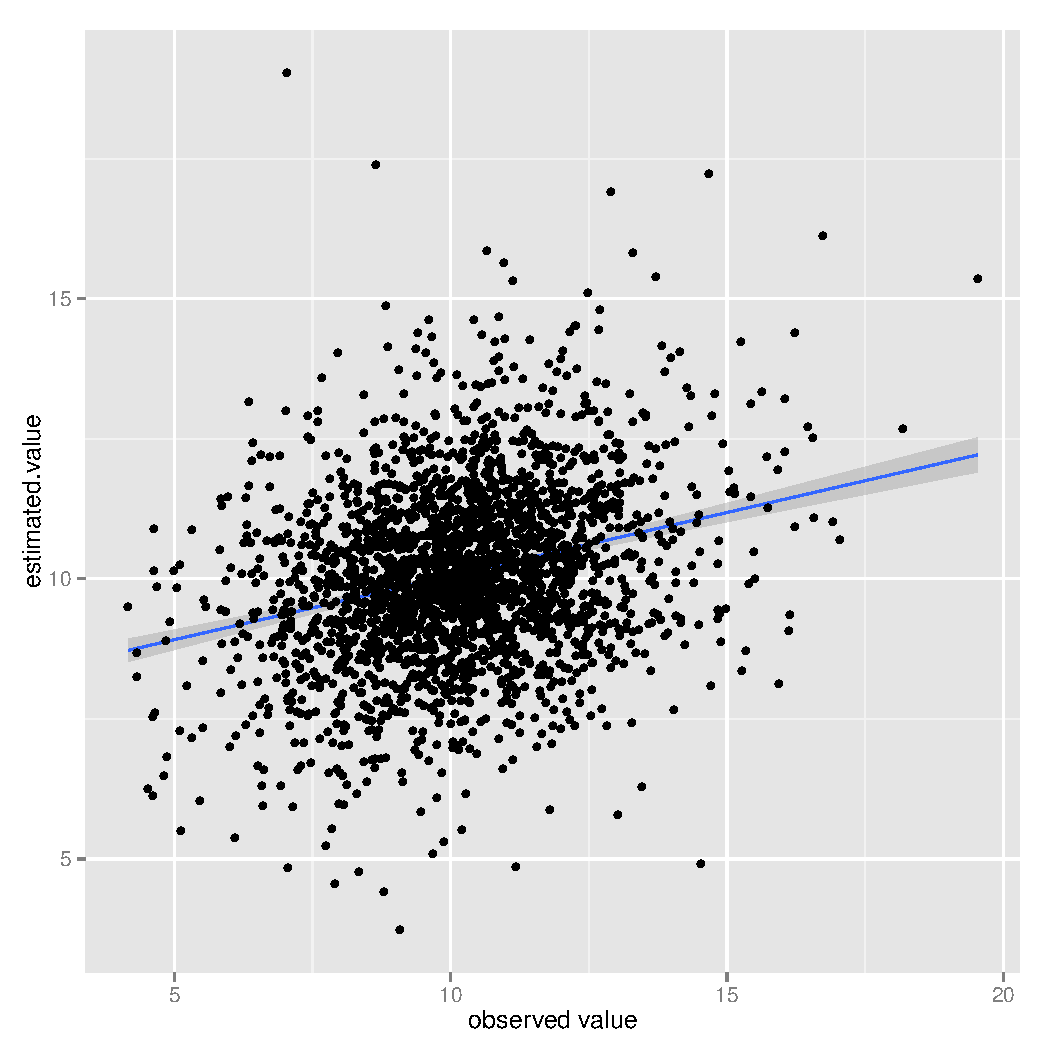
\includegraphics[width=.6\textwidth]{figures/PPBstats_unnamed-chunk-42-1} 

}



\end{knitrout}
\end{figure}


\subsubsection{Perform cross validation studies}

This step is useful to assess the quality of the model.
This step is higly computing consuming as the FWH model is run as many time as there is value of $Y_{ij}$ (i.e. number of rows of the data set).

The complete cross validation is done with \texttt{cross.validation.FWH}: 
each Value of $Y_{ij}$ is estimated by the entire data set without this value.

The convergence is not check for each validation. 
If the parameters in the FWH converge, then it is assumed that the FWH in the cross validation converge as well.

The model is run on dataset where germplasms are in three environments at least so the smallest data set where the cross valisation is run has germplasms present in two environments at least. 

You may parallelise to gain time with the \texttt{mc.cores} argument of the function.

The number of iterations is set to 100 000 but you can change it with the \texttt{nb\_iterations} argument.

The percentage of confidence is calculated with a t-test:

\begin{displaymath}
t = \frac{m - 0}{s/\sqrt{N}}
\end{displaymath}
with,

$N$ the number of observations in the data set,

$m = \frac{1}{N} \sum\limits_{n=1}^N Y_{n} - \hat{Y_{n}}$, the average bias

$s = \sqrt{\frac{1}{N-1} \sum\limits_{n=1}^N (Y_{n} - \hat{Y_{n}})^2}$, the standard deviation of the bias

$t$ follows a Student distribution with $N-1$ degree of freedom.

The percentage of confidence (i.e. the probability $H0$: the bias is equal to zero) comes from this distribution.

A regression is also done between estimated and observed value.

Here it is bad as only 10 iterations have been done to save computing time ...

\begin{knitrout}
\definecolor{shadecolor}{rgb}{0.969, 0.969, 0.969}\color{fgcolor}\begin{kframe}
\begin{alltt}
\hlcom{# out.cv = cross.validation.FWH(data = PPBdata2, variable = "y1", nb_iterations = 10)}
\hlkwd{load}\hlstd{(}\hlstr{"./data_PPBstats/out.cv.RData"}\hlstd{)} \hlcom{# to save lots of time}
\end{alltt}
\end{kframe}
\end{knitrout}

\begin{knitrout}
\definecolor{shadecolor}{rgb}{0.969, 0.969, 0.969}\color{fgcolor}\begin{kframe}
\begin{alltt}
\hlstd{out.cv}\hlopt{$}\hlstd{percentage.of.confidence}
\end{alltt}
\begin{verbatim}
## [1] 6.7
\end{verbatim}
\end{kframe}
\end{knitrout}

\begin{figure}[H]
\begin{knitrout}
\definecolor{shadecolor}{rgb}{0.969, 0.969, 0.969}\color{fgcolor}\begin{kframe}
\begin{alltt}
\hlstd{out.cv}\hlopt{$}\hlstd{regression}
\end{alltt}
\begin{verbatim}
## $plot
\end{verbatim}


{\ttfamily\noindent\color{warningcolor}{\#\# Warning in loop\_apply(n, do.ply): Removed 1 rows containing missing values (stat\_smooth).}}

{\ttfamily\noindent\color{warningcolor}{\#\# Warning in loop\_apply(n, do.ply): Removed 1 rows containing missing values (geom\_point).}}\begin{verbatim}
## 
## $anova
## 
## Call:
## lm(formula = real.value ~ estimated.value)
## 
## Coefficients:
##     (Intercept)  estimated.value  
##          6.8640           0.3275
\end{verbatim}
\end{kframe}

{\centering 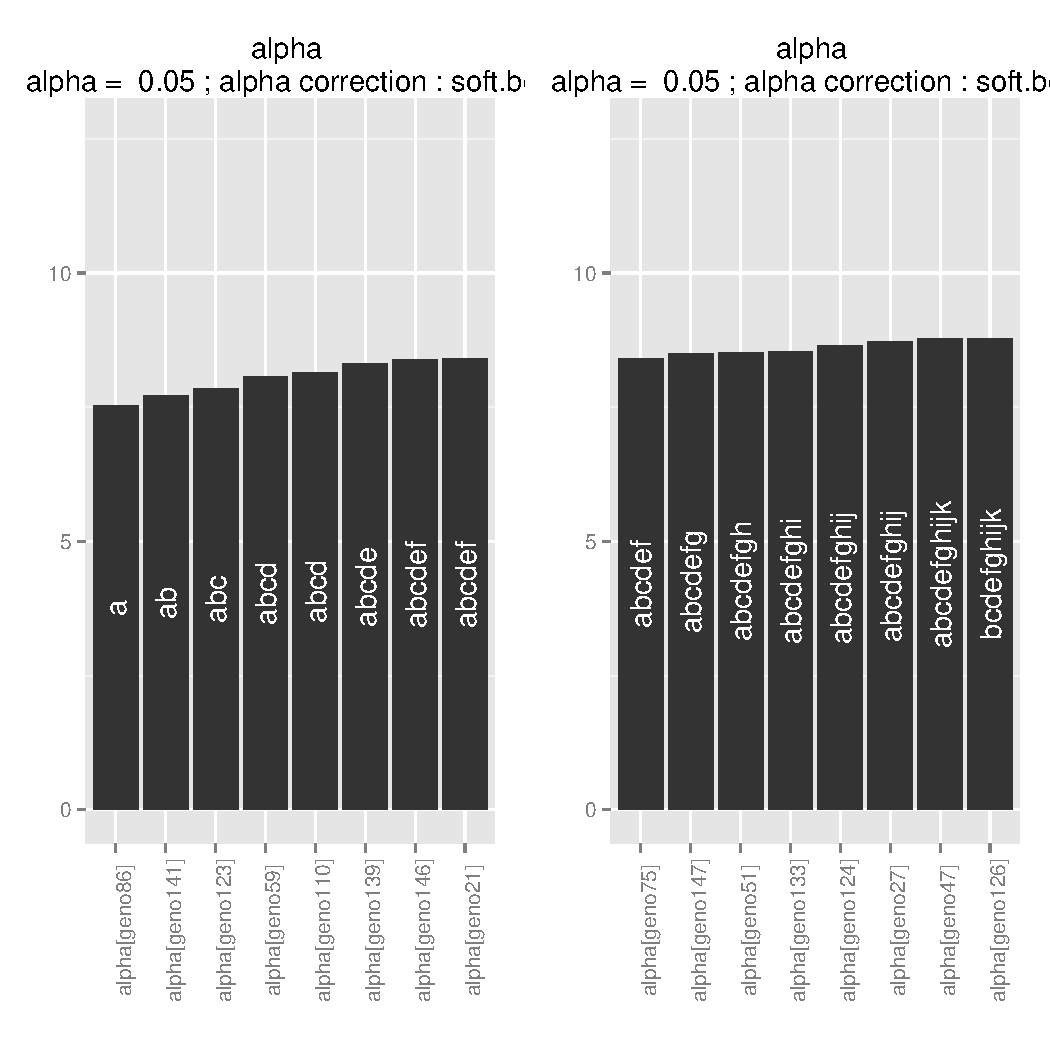
\includegraphics[width=.6\textwidth]{figures/PPBstats_unnamed-chunk-45-1} 

}



\end{knitrout}
\end{figure}



\subsubsection{Get mean comparisons}
For mean comparisons of parameters, it is the same method that presented in section \ref{mean_comp}.

\begin{knitrout}
\definecolor{shadecolor}{rgb}{0.969, 0.969, 0.969}\color{fgcolor}\begin{kframe}
\begin{alltt}
\hlstd{comp.alpha} \hlkwb{=} \hlkwd{get.mean.comparisons}\hlstd{(out2}\hlopt{$}\hlstd{MCMC,} \hlstr{"alpha"}\hlstd{)}
\hlstd{comp.theta} \hlkwb{=} \hlkwd{get.mean.comparisons}\hlstd{(out2}\hlopt{$}\hlstd{MCMC,} \hlstr{"theta"}\hlstd{)}
\hlstd{comp.beta} \hlkwb{=} \hlkwd{get.mean.comparisons}\hlstd{(out2}\hlopt{$}\hlstd{MCMC,} \hlstr{"beta"}\hlstd{,} \hlkwc{type} \hlstd{=} \hlnum{2}\hlstd{,} \hlkwc{threshold} \hlstd{=} \hlnum{1}\hlstd{)}
\end{alltt}
\end{kframe}
\end{knitrout}

To see the output, use \texttt{get.ggplot}.

\begin{knitrout}
\definecolor{shadecolor}{rgb}{0.969, 0.969, 0.969}\color{fgcolor}\begin{kframe}
\begin{alltt}
\hlstd{p_barplot} \hlkwb{=} \hlkwd{get.ggplot}\hlstd{(comp.alpha,} \hlkwc{ggplot.type} \hlstd{=} \hlstr{"barplot"}\hlstd{)}
\end{alltt}
\end{kframe}
\end{knitrout}

Lets' have a look at the firt values of $\alpha_i$.

\begin{figure}[H]
\begin{knitrout}
\definecolor{shadecolor}{rgb}{0.969, 0.969, 0.969}\color{fgcolor}\begin{kframe}
\begin{alltt}
\hlkwd{grid.arrange}\hlstd{(p_barplot}\hlopt{$}\hlstr{"alpha"}\hlstd{[[}\hlnum{1}\hlstd{]], p_barplot}\hlopt{$}\hlstr{"alpha"}\hlstd{[[}\hlnum{2}\hlstd{]] ,} \hlkwc{ncol} \hlstd{=} \hlnum{2}\hlstd{,} \hlkwc{nrow} \hlstd{=} \hlnum{1}\hlstd{)}
\end{alltt}
\end{kframe}

{\centering 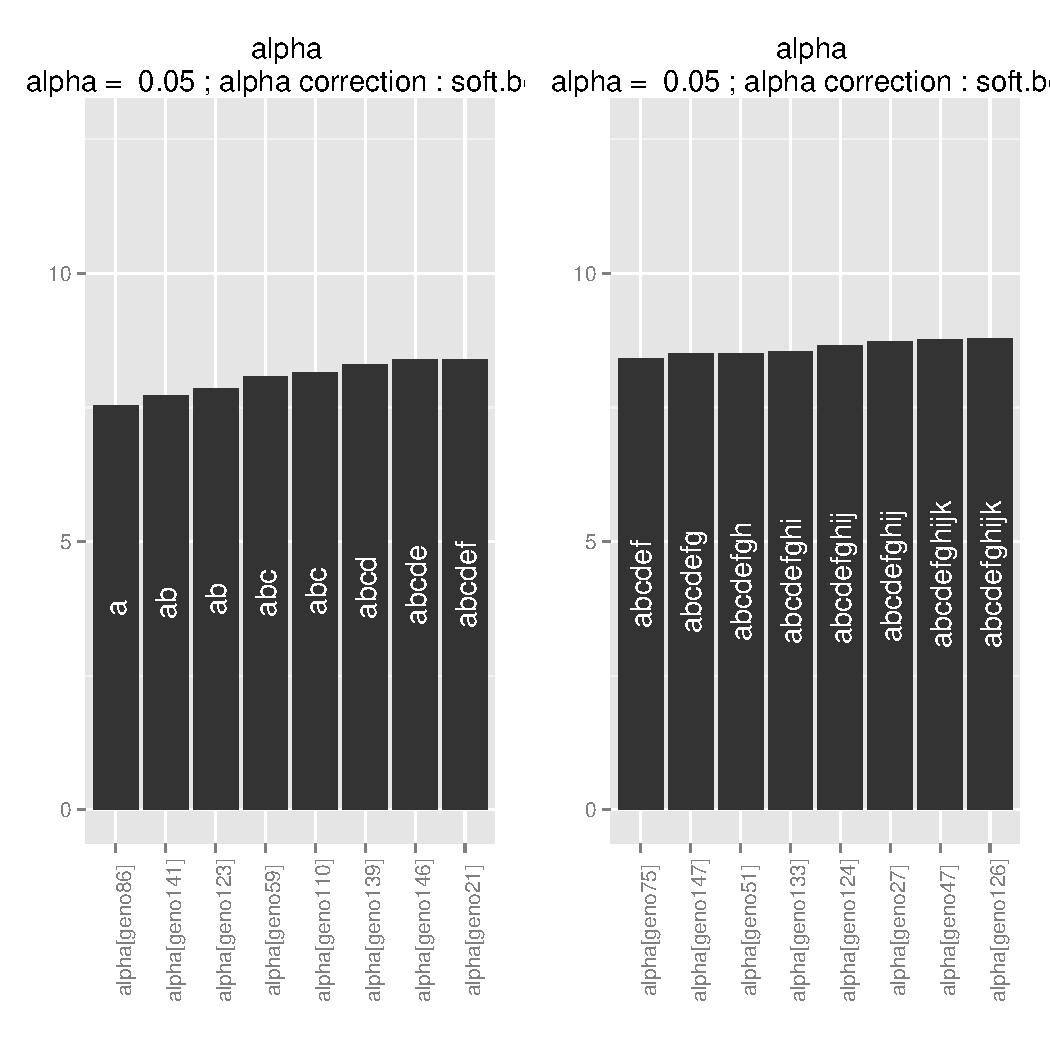
\includegraphics[width=.6\textwidth]{figures/PPBstats_unnamed-chunk-48-1} 

}



\end{knitrout}
\end{figure}

\subsubsection{Get biplot $\beta = f(\alpha)$}

It is interessting to compare genetic effect versus sensibility to interaction.
A germplasm with an high genetic effect and a low sensitivity to interaction (i.e. close to 0) may be a good candidate to sown.

\begin{knitrout}
\definecolor{shadecolor}{rgb}{0.969, 0.969, 0.969}\color{fgcolor}\begin{kframe}
\begin{alltt}
\hlstd{comp.alpha} \hlkwb{=} \hlkwd{get.mean.comparisons}\hlstd{(out2}\hlopt{$}\hlstd{MCMC,} \hlstr{"alpha"}\hlstd{)}
\hlstd{comp.beta} \hlkwb{=} \hlkwd{get.mean.comparisons}\hlstd{(out2}\hlopt{$}\hlstd{MCMC,} \hlstr{"beta"}\hlstd{)}

\hlstd{g} \hlkwb{=} \hlkwd{get.ggplot}\hlstd{(}\hlkwc{data} \hlstd{= comp.alpha,} \hlkwc{data_2} \hlstd{= comp.beta,} \hlkwc{ggplot.type} \hlstd{=} \hlstr{"biplot-alpha-beta"}\hlstd{)}
\hlstd{g}\hlopt{$}\hlstd{biplot}
\end{alltt}
\end{kframe}

{\centering 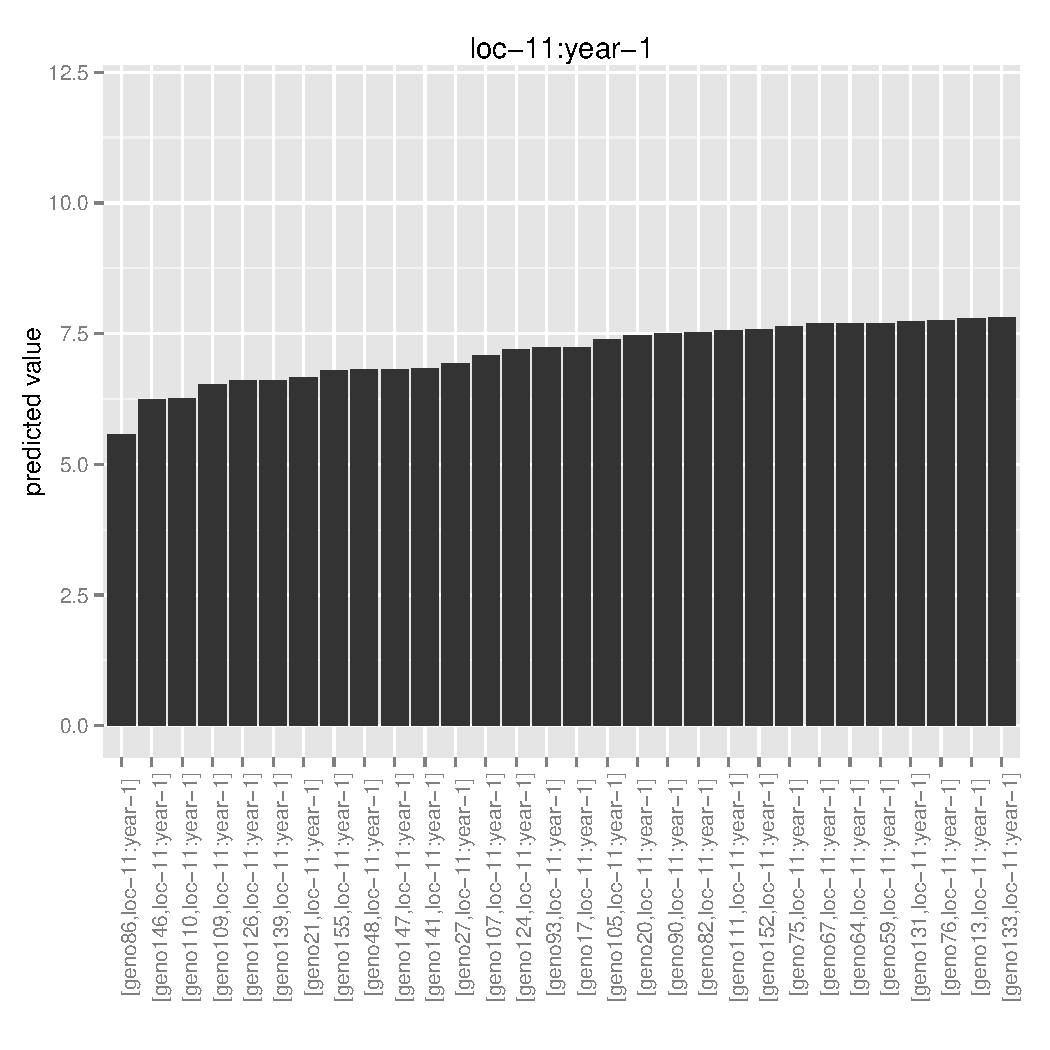
\includegraphics[width=.6\textwidth]{figures/PPBstats_unnamed-chunk-49-1} 

}



\end{knitrout}


\subsubsection{Get groups of parameters}

In order to cluster environments or germplasms, you may use mulivariate analysis on a matrix with several variables in columns and parameter in rows.

This is done with \texttt{get.parameter.groups} which do a PCA on this matrix and then find cluster with the \texttt{HCPC} procedure from package \texttt{FactoMineR}: it is a K-means clustering that creates clusters of similar parameters \citep{husson_principal_2010}.
The Kmeans clustering was done on the first two axes of the PCA that represented the main information while the last axes represented mainly noise \citep{husson_principal_2010}.
The number of clusters is choosen to maximise the variance between clusters and within clusters.
For more information type \texttt{?get.parameter.groups}.

\begin{knitrout}
\definecolor{shadecolor}{rgb}{0.969, 0.969, 0.969}\color{fgcolor}\begin{kframe}
\begin{alltt}
\hlcom{# out.model2_y1 = FWH(PPBdata2, variable = "y1")}
\hlkwd{load}\hlstd{(}\hlstr{"./data_PPBstats/out.model2_y1.RData"}\hlstd{)} \hlcom{# to save time}

\hlcom{# out.model2_y2 = FWH(PPBdata2, variable = "y2")}
\hlkwd{load}\hlstd{(}\hlstr{"./data_PPBstats/out.model2_y2.RData"}\hlstd{)} \hlcom{# to save time}

\hlcom{# out.model2_y3 = FWH(PPBdata2, variable = "y3")}
\hlkwd{load}\hlstd{(}\hlstr{"./data_PPBstats/out.model2_y3.RData"}\hlstd{)} \hlcom{# to save time}

\hlstd{out2_y1} \hlkwb{=} \hlkwd{analyse.outputs}\hlstd{(out.model2_y1)}
\end{alltt}


{\ttfamily\noindent\itshape\color{messagecolor}{\#\# The experimental design plot is done.\\\#\# The Gelman-Rubin test is running for each parameter ...\\\#\# The two MCMC for each parameter converge thanks to the Gelman-Rubin test.\\\#\# The alpha\_i posterior distributions are done.\\\#\# The beta\_i posterior distributions are done.\\\#\# The theta\_j posterior distributions are done.}}\begin{alltt}
\hlstd{out2_y2} \hlkwb{=} \hlkwd{analyse.outputs}\hlstd{(out.model2_y2)}
\end{alltt}


{\ttfamily\noindent\itshape\color{messagecolor}{\#\# The experimental design plot is done.\\\#\# The Gelman-Rubin test is running for each parameter ...\\\#\# The two MCMC for each parameter converge thanks to the Gelman-Rubin test.\\\#\# The alpha\_i posterior distributions are done.\\\#\# The beta\_i posterior distributions are done.\\\#\# The theta\_j posterior distributions are done.}}\begin{alltt}
\hlstd{out2_y3} \hlkwb{=} \hlkwd{analyse.outputs}\hlstd{(out.model2_y3)}
\end{alltt}


{\ttfamily\noindent\itshape\color{messagecolor}{\#\# The experimental design plot is done.\\\#\# The Gelman-Rubin test is running for each parameter ...\\\#\# The two MCMC for each parameter converge thanks to the Gelman-Rubin test.\\\#\# The alpha\_i posterior distributions are done.\\\#\# The beta\_i posterior distributions are done.\\\#\# The theta\_j posterior distributions are done.}}\begin{alltt}
\hlstd{analyse.outputs.list} \hlkwb{=} \hlkwd{list}\hlstd{(}\hlkwc{var1} \hlstd{= out2_y1,} \hlkwc{var2} \hlstd{= out2_y2,} \hlkwc{var3} \hlstd{= out2_y3)}

\hlstd{clust} \hlkwb{=} \hlkwd{get.parameter.groups}\hlstd{(analyse.outputs.list,} \hlkwc{parameter} \hlstd{=} \hlstr{"theta"}\hlstd{)}
\end{alltt}
\end{kframe}
\end{knitrout}

To see the output, use \texttt{get.ggplot}.
A farmer may find a germplasm that behaves well according to informations from model \ref{model1} (section \ref{section_model1}) in a farm that shares its cluster.

\begin{figure}[H]
\begin{knitrout}
\definecolor{shadecolor}{rgb}{0.969, 0.969, 0.969}\color{fgcolor}\begin{kframe}
\begin{alltt}
\hlstd{p_PCA} \hlkwb{=} \hlkwd{get.ggplot}\hlstd{(clust,} \hlkwc{ggplot.type} \hlstd{=} \hlstr{"PCA"}\hlstd{)}
\hlstd{p_PCA}
\end{alltt}
\begin{verbatim}
## $ind
## 
## $var
\end{verbatim}
\end{kframe}


{\centering 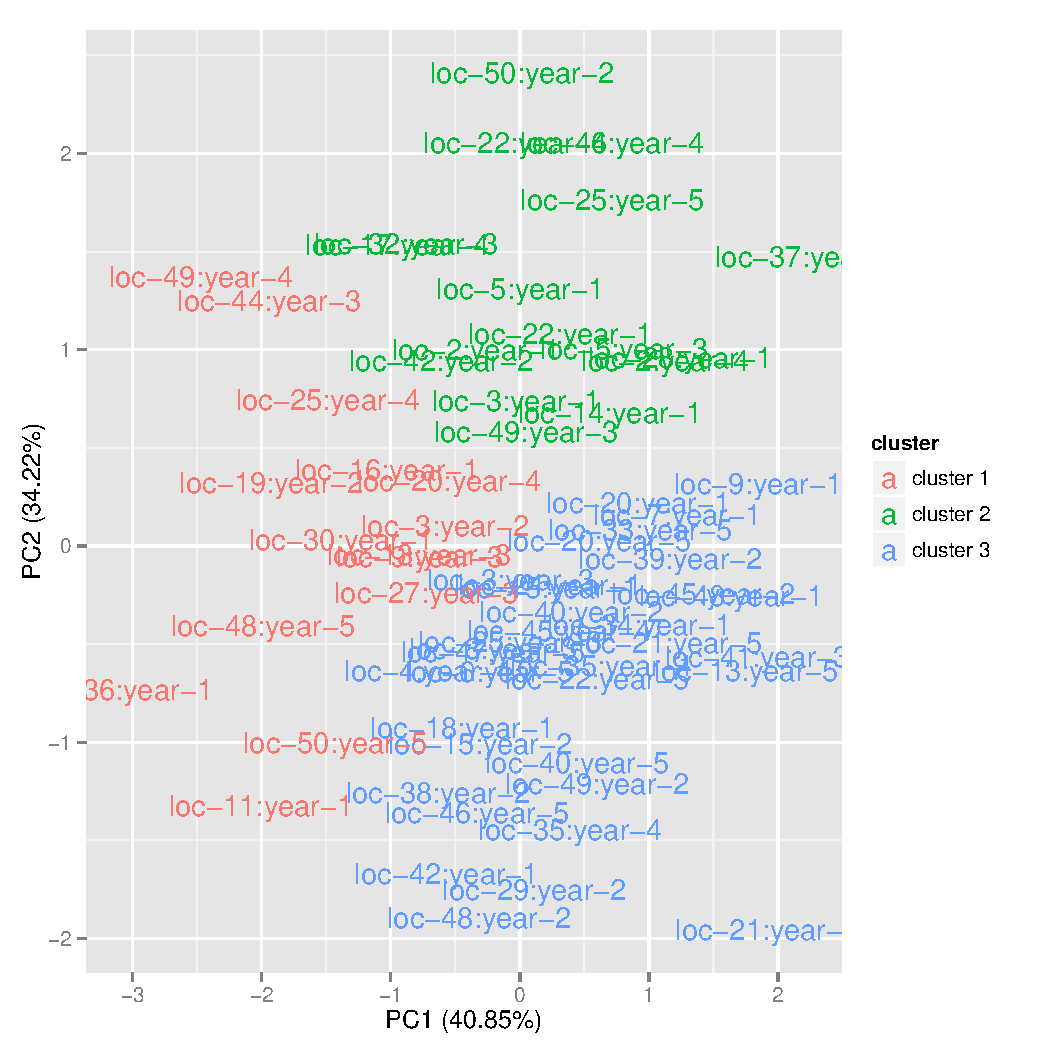
\includegraphics[width=.6\textwidth]{figures/PPBstats_unnamed-chunk-51-1} 
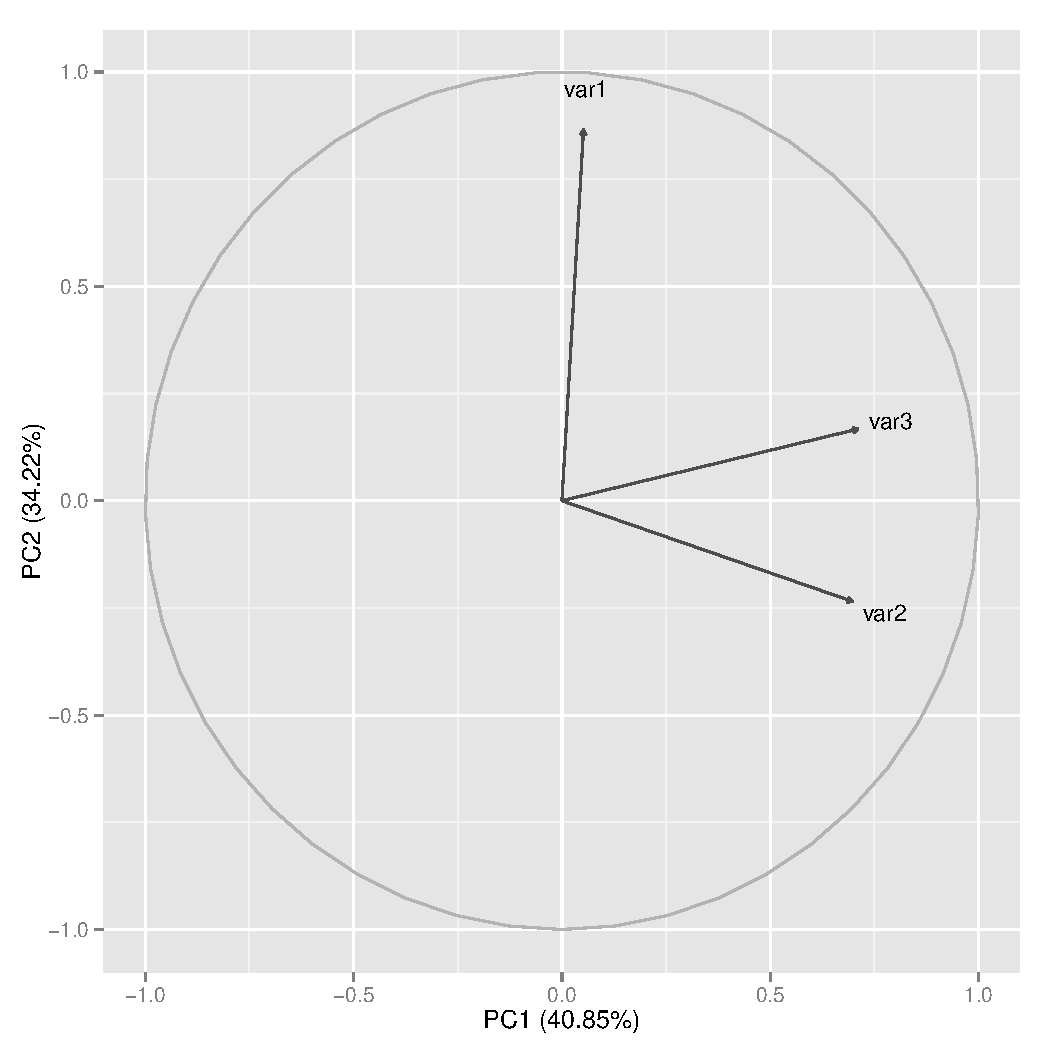
\includegraphics[width=.6\textwidth]{figures/PPBstats_unnamed-chunk-51-2} 

}



\end{knitrout}
\end{figure}



\subsubsection{Predict the past}

In order to choose a new germplasm to test on his farm, a farmer may choose a germplasm according to the value it would have obtained on his farm.

You may either get the estimated MCMC, but you will need lots of memory, or the summary statistics of the MCMC.

Due to memory issues, it may be better to choose output.format = "summary".
This allows caterpillar plots but no mean comparisons that are base on the whole MCMC.

\begin{knitrout}
\definecolor{shadecolor}{rgb}{0.969, 0.969, 0.969}\color{fgcolor}\begin{kframe}
\begin{alltt}
\hlcom{# out.predict.the.past = predict.the.past(out2, output.format = "summary")}
\hlcom{# |==========================================================| 100%}
\hlkwd{load}\hlstd{(}\hlstr{"./data_PPBstats/out.predict.the.past.RData"}\hlstd{)} \hlcom{# to save time}
\hlkwd{dim}\hlstd{(out.predict.the.past)}
\end{alltt}
\begin{verbatim}
## [1] 8140    8
\end{verbatim}
\end{kframe}
\end{knitrout}


If you choose \texttt{output.format = "summary"}, it is possible to look at the results with \texttt{get.ggplot}.


\begin{knitrout}
\definecolor{shadecolor}{rgb}{0.969, 0.969, 0.969}\color{fgcolor}\begin{kframe}
\begin{alltt}
\hlstd{p_barplot_predict} \hlkwb{=} \hlkwd{get.ggplot}\hlstd{(out.predict.the.past,} \hlkwc{ggplot.type} \hlstd{=} \hlstr{"barplot"}\hlstd{,}
                               \hlkwc{nb_parameters_per_plot} \hlstd{=} \hlnum{30}\hlstd{)}
\hlstd{p_barplot_predict}\hlopt{$}\hlstd{`loc-11:year-1`}\hlopt{$}\hlstd{`1`}
\end{alltt}
\end{kframe}

{\centering 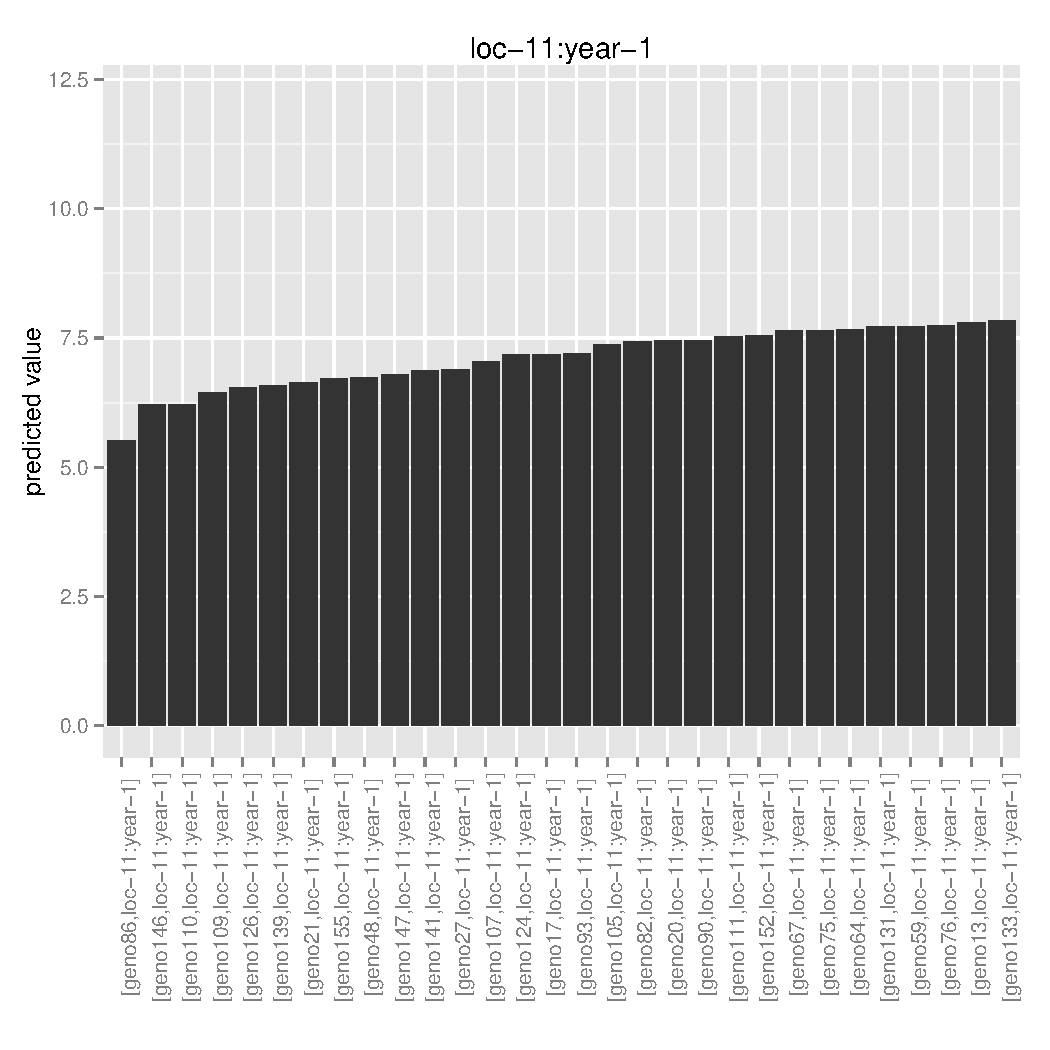
\includegraphics[width=.6\textwidth]{figures/PPBstats_unnamed-chunk-53-1} 

}



\end{knitrout}

\begin{knitrout}
\definecolor{shadecolor}{rgb}{0.969, 0.969, 0.969}\color{fgcolor}\begin{kframe}
\begin{alltt}
\hlstd{p_interaction_predict} \hlkwb{=} \hlkwd{get.ggplot}\hlstd{(out.predict.the.past,} \hlkwc{ggplot.type} \hlstd{=} \hlstr{"interaction"}\hlstd{)}
\hlstd{p_interaction_predict}\hlopt{$}\hlstd{`loc-46`}\hlopt{$}\hlstd{`1`}
\end{alltt}
\end{kframe}

{\centering 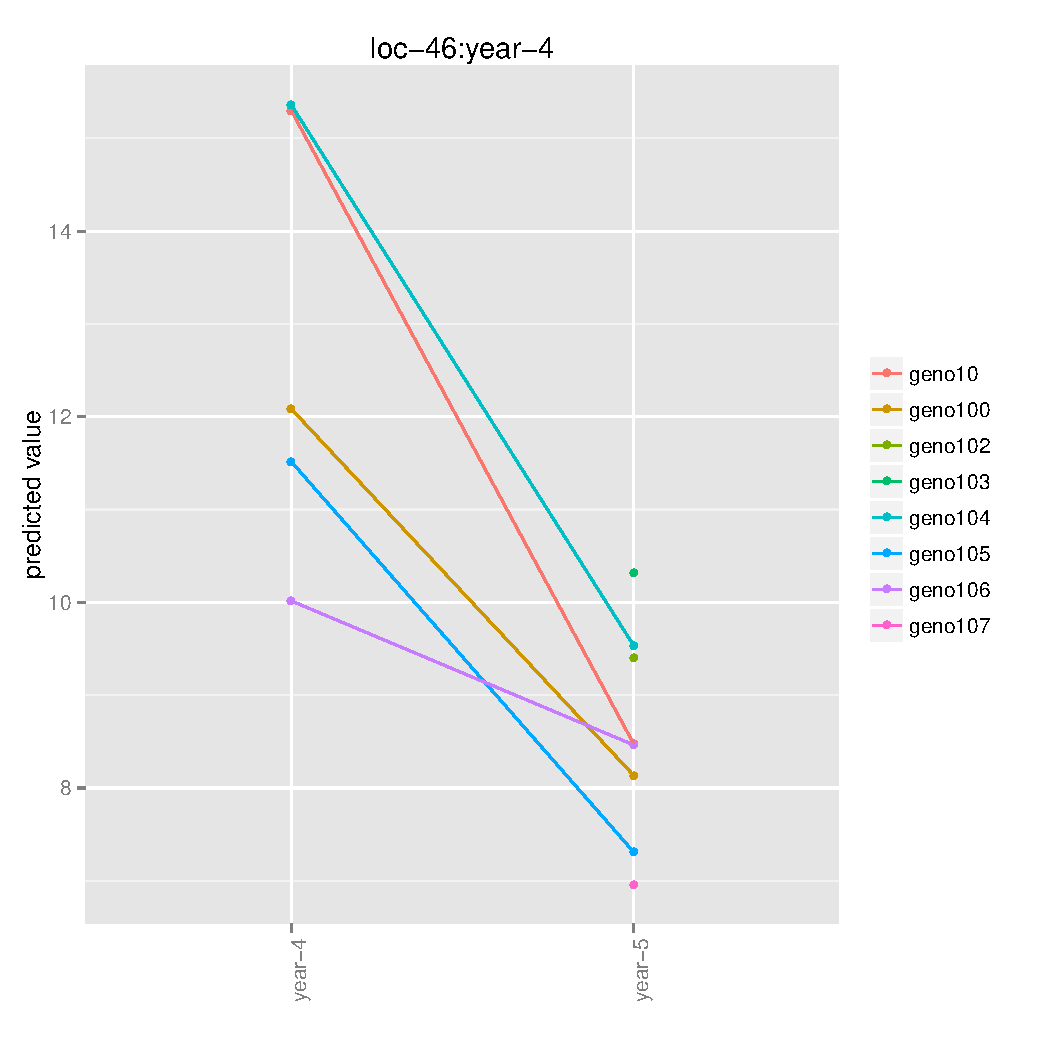
\includegraphics[width=.6\textwidth]{figures/PPBstats_unnamed-chunk-54-1} 

}



\end{knitrout}



\newpage

\section*{To cite \pack} \addcontentsline{toc}{section}{To cite \pack}
To cite this package and or this vignette:

\begin{knitrout}
\definecolor{shadecolor}{rgb}{0.969, 0.969, 0.969}\color{fgcolor}\begin{kframe}
\begin{alltt}
\hlkwd{citation}\hlstd{(}\hlstr{"PPBstats"}\hlstd{)}
\end{alltt}
\begin{verbatim}
## 
## To cite the PPBstats package in publications use:
## 
##   Pierre Riviere and Olivier David, 2016, PPBstats: An R
##   package for statistical analysis of unbalanced trials in
##   decentralized participatory plant breeding programmes.
##   Version 0.11.0, URL: https://github.com/priviere/PPBstats
## 
## A BibTeX entry for LaTeX users is
## 
##   @Manual{,
##     title = {PPBstats: An R package for statistical analysis 
##           of unbalanced trials in decentralized participatory plant 
##           breeding programmes. Version 0.11.0},
##     author = {{Pierre Riviere and Olivier David}},
##     organisation = {{Reseau Semences Paysannes}, {INRA}},
##     year = {2016},
##     url = {https://github.com/priviere/PPBstats},
##     note = {R code is under licence GPL-3. 
##           Vignette is under licence creative commons BY-NC-SA 4.0.},
##   }
\end{verbatim}
\end{kframe}
\end{knitrout}



\chapter*{Aknowledgement} \addcontentsline{toc}{chapter}{Aknowledgement}
This worked has been first funded by the European Community’s Seventh Framework Programme (FP7/9 2007–2013) under the grant agreement n245058-Solibam (Strategies for Organic and Low-input Integrated Breeding and Management).
It has been completed by funding from European Union’s Horizon 2020 research and innovation programme under grant agreement No 633571 (DIVERSIFOOD project) and Fondation de France.


\begin{center}

\includegraphics[width=.28\textwidth]{Logo-Diversifood} \hspace{.5cm}

\includegraphics[width=.18\textwidth]{Logo-SOLIBAM} \hspace{.5cm}

\includegraphics[width=.2\textwidth]{Logo-EU} \hspace{.5cm}

\includegraphics[width=.18\textwidth]{Logo-FdF}
\end{center}

Thanks to Hadley Wickham for his web site \url{http://r-pkgs.had.co.nz/} that help us a lot in the creation of this package.
Thanks to Jonathan Locqueville and Maxime Garnault that work during their internship on a first version of the AMMI code.
Thanks to Salvatore Ceccarelli for its useful comments and references on data analysis and software.
Thanks to Jérôme Dury for spelling corrections of the vignette.

\bibliography{biblio} \addcontentsline{toc}{chapter}{References}
\bibliographystyle{plainnat}


\end{document}

